% Generated fragments require trusted human review before compilation.
% This binder never requests shell escape or runs external tools.
\documentclass[11pt]{article}
% Trusted shared apparatus. Requires LuaLaTeX; never use shell escape.
\usepackage{fontspec}
\defaultfontfeatures{Ligatures=TeX}
\IfFontExistsTF{Noto Serif}{\setmainfont{Noto Serif}}{%
  \IfFontExistsTF{DejaVu Serif}{\setmainfont{DejaVu Serif}}{%
    \IfFontExistsTF{Times New Roman}{\setmainfont{Times New Roman}}{%
      \PackageError{gelfand-binder}{No configured Cyrillic serif font installed}{Install Noto Serif or DejaVu Serif, or select an installed Cyrillic font.}%
    }%
  }%
}
\IfFontExistsTF{Noto Sans}{\setsansfont{Noto Sans}}{%
  \IfFontExistsTF{DejaVu Sans}{\setsansfont{DejaVu Sans}}{\setsansfont{Arial}}%
}
\IfFontExistsTF{Noto Sans Mono}{\setmonofont{Noto Sans Mono}}{%
  \IfFontExistsTF{DejaVu Sans Mono}{\setmonofont{DejaVu Sans Mono}}{\setmonofont{Courier New}}%
}
\usepackage[a4paper,margin=22mm]{geometry}
\usepackage{amsmath,amssymb,amsthm,mathtools}
\usepackage{xcolor}
\usepackage{tikz}
\usepackage{tikz-cd}
\usetikzlibrary{arrows.meta,positioning,calc}
\usepackage{hyperref}
\hypersetup{unicode=true,colorlinks=true,linkcolor=blue,pdftitle={Gelfand transcription binder}}
\newtheorem{theorem}{Theorem}
\newtheorem{lemma}{Lemma}
\newtheorem{proposition}{Proposition}
\newtheorem{corollary}{Corollary}
\theoremstyle{definition}
\newtheorem{definition}{Definition}
\newtheorem{example}{Example}
\theoremstyle{remark}
\newtheorem{remark}{Remark}
\setlength{\parindent}{0pt}
\setlength{\parskip}{0.55em}
\setlength{\emergencystretch}{3em}
\newcommand{\SourcePage}[2]{%
  \clearpage\phantomsection\label{#1:source-page}%
  \addcontentsline{toc}{subsection}{#1}%
  {\small\sffamily\color{blue!60!black}Source scan frame: #1; visible page/leaf label: #2}\par\medskip%
}
\newcommand{\Unclear}[3]{%
  \begingroup\color{orange!70!black}%
  [Unresolved reading #1/#2: #3]\endgroup%
}
\newcommand{\Incomplete}[3]{%
  \par\begingroup\color{red!65!black}\textbf{Incomplete #1/#2:} #3\endgroup\par%
}
\newcommand{\SourceFigure}[3]{%
  \par\begingroup\color{blue!60!black}\textbf{\hyperref[#1:source-page]{Source figure #1/#2}:} #3%
  \par\textit{Consult the authoritative scan at this locator.}\endgroup\par%
}



% Reader layout only. Original diplomatic text is retained verbatim.
\setlength{\parskip}{0.35em}
\setlength{\emergencystretch}{4em}
\renewcommand{\SourcePage}[2]{%
  \par\addvspace{1em}\phantomsection\label{#1:source-page}%
  \addcontentsline{toc}{subsection}{#1}%
  {\footnotesize\sffamily\color{blue!55!black}#1%
    \def\givenlabel{#2}\def\nolabel{unlabelled}%
    \ifx\givenlabel\nolabel\else\quad[номер в источнике: #2]\fi
  }\par\nobreak\smallskip%
}
\renewcommand{\Unclear}[3]{%
  \begingroup\color{orange!65!black}%
  \ifmmode\text{[неясно: #3]}\else[неясно: #3]\fi\endgroup%
}
\renewcommand{\Incomplete}[3]{%
  \par\begingroup\color{red!60!black}\textbf{Неразобранный фрагмент:} #3%
  \endgroup\par%
}
\renewcommand{\SourceFigure}[3]{%
  \par\begingroup\color{blue!55!black}\textbf{Рисунок:} #3%
  \par{\small\textit{Исходный рисунок: \hyperref[#1:source-page]{#1}, #2.}}%
  \endgroup\par%
}
\hypersetup{pdftitle={Семинар И. М. Гельфанда. Дипломатическая транскрипция},pdfauthor={},pdfsubject={Русское рабочее издание с отмеченными сомнительными чтениями}}

\usepackage[normalem]{ulem}
\usepackage{newunicodechar}
\usepackage{adjustbox}
\newfontfamily\SourceSymbolFont{Segoe UI Symbol}
\newfontfamily\SourceCJKFont{MS Gothic}
\let\DiplomaticMathUnderline\underline
\renewcommand{\underline}[1]{\ifmmode\DiplomaticMathUnderline{#1}\else\uline{#1}\fi}
\newunicodechar{→}{\ifmmode\text{{\SourceSymbolFont\char"2192}}\else{\SourceSymbolFont\char"2192}\fi}
\newunicodechar{⇒}{\ifmmode\text{{\SourceSymbolFont\char"21D2}}\else{\SourceSymbolFont\char"21D2}\fi}
\newunicodechar{∀}{\ifmmode\text{{\SourceSymbolFont\char"2200}}\else{\SourceSymbolFont\char"2200}\fi}
\newunicodechar{∂}{\ifmmode\text{{\SourceSymbolFont\char"2202}}\else{\SourceSymbolFont\char"2202}\fi}
\newunicodechar{∈}{\ifmmode\text{{\SourceSymbolFont\char"2208}}\else{\SourceSymbolFont\char"2208}\fi}
\newunicodechar{∌}{\ifmmode\text{{\SourceSymbolFont\char"220C}}\else{\SourceSymbolFont\char"220C}\fi}
\newunicodechar{√}{\ifmmode\text{{\SourceSymbolFont\char"221A}}\else{\SourceSymbolFont\char"221A}\fi}
\newunicodechar{∞}{\ifmmode\text{{\SourceSymbolFont\char"221E}}\else{\SourceSymbolFont\char"221E}\fi}
\newunicodechar{∧}{\ifmmode\text{{\SourceSymbolFont\char"2227}}\else{\SourceSymbolFont\char"2227}\fi}
\newunicodechar{∩}{\ifmmode\text{{\SourceSymbolFont\char"2229}}\else{\SourceSymbolFont\char"2229}\fi}
\newunicodechar{∪}{\ifmmode\text{{\SourceSymbolFont\char"222A}}\else{\SourceSymbolFont\char"222A}\fi}
\newunicodechar{∫}{\ifmmode\text{{\SourceSymbolFont\char"222B}}\else{\SourceSymbolFont\char"222B}\fi}
\newunicodechar{∴}{\ifmmode\text{{\SourceSymbolFont\char"2234}}\else{\SourceSymbolFont\char"2234}\fi}
\newunicodechar{∼}{\ifmmode\text{{\SourceSymbolFont\char"223C}}\else{\SourceSymbolFont\char"223C}\fi}
\newunicodechar{≈}{\ifmmode\text{{\SourceSymbolFont\char"2248}}\else{\SourceSymbolFont\char"2248}\fi}
\newunicodechar{≠}{\ifmmode\text{{\SourceSymbolFont\char"2260}}\else{\SourceSymbolFont\char"2260}\fi}
\newunicodechar{≤}{\ifmmode\text{{\SourceSymbolFont\char"2264}}\else{\SourceSymbolFont\char"2264}\fi}
\newunicodechar{≥}{\ifmmode\text{{\SourceSymbolFont\char"2265}}\else{\SourceSymbolFont\char"2265}\fi}
\newunicodechar{⊕}{\ifmmode\text{{\SourceSymbolFont\char"2295}}\else{\SourceSymbolFont\char"2295}\fi}
\newunicodechar{⊗}{\ifmmode\text{{\SourceSymbolFont\char"2297}}\else{\SourceSymbolFont\char"2297}\fi}
\newunicodechar{①}{\ifmmode\text{{\SourceSymbolFont\char"2460}}\else{\SourceSymbolFont\char"2460}\fi}
\newunicodechar{②}{\ifmmode\text{{\SourceSymbolFont\char"2461}}\else{\SourceSymbolFont\char"2461}\fi}
\newunicodechar{③}{\ifmmode\text{{\SourceSymbolFont\char"2462}}\else{\SourceSymbolFont\char"2462}\fi}
\newunicodechar{④}{\ifmmode\text{{\SourceSymbolFont\char"2463}}\else{\SourceSymbolFont\char"2463}\fi}
\newunicodechar{Ⓗ}{\ifmmode\text{{\SourceSymbolFont\char"24BD}}\else{\SourceSymbolFont\char"24BD}\fi}
\newunicodechar{〃}{\ifmmode\text{{\SourceCJKFont\char"3003}}\else{\SourceCJKFont\char"3003}\fi}


% Reader revision 3. Annotation wording and candidates remain unchanged.
\setmainfont{NotoSerif-Regular.ttf}[Path=C:/Windows/Fonts/,ItalicFont=NotoSerif-Italic.ttf,BoldFont=NotoSerif-Bold.ttf,BoldItalicFont=NotoSerif-BoldItalic.ttf]
\usetikzlibrary{shapes.geometric,decorations.pathreplacing,decorations.markings,patterns,fit}
\newsavebox{\ReaderAnnotationBox}
\newcommand{\ReaderAnnotation}[1]{%
  \sbox{\ReaderAnnotationBox}{[неясно: #1]}%
  \ifdim\wd\ReaderAnnotationBox>.70\linewidth
    \parbox[t]{.70\linewidth}{\raggedright[неясно: #1]}%
  \else\usebox{\ReaderAnnotationBox}\fi%
}
\ExplSyntaxOn
\cs_new_protected:Npn \reader_unclear_candidate:n #1
 {
  \tl_set:Nx \l_tmpa_tl { \tl_to_str:n {#1} }
  % Text explicitly guarded inside a mathematical candidate remains math-safe.
  \regex_replace_all:nnN { \\(?:text|textrm|textnormal|textbf|operatorname)\s*\{[^{}]*\} } { } \l_tmpa_tl
  \regex_match:nVTF { [\x{0400}-\x{052F}] | \$ } \l_tmpa_tl
   { \ifmmode \text{\ReaderAnnotation{#1}} \else \ReaderAnnotation{#1} \fi }
   {
    \ifmmode
      [\text{неясно:~}#1]
    \else
      \regex_match:nVTF { [_^] | \\ } \l_tmpa_tl
       { \ensuremath{[\text{неясно:~}#1]} }
       { \ReaderAnnotation{#1} }
    \fi
   }
 }
\RenewDocumentCommand \Unclear { m m m }
 { \begingroup\color{orange!65!black}\reader_unclear_candidate:n{#3}\endgroup }
\ExplSyntaxOff
\newsavebox{\ReaderIncompleteBox}
\newcommand{\ReaderIncompleteNote}[1]{%
 \sbox{\ReaderIncompleteBox}{\textbf{Неразобранный фрагмент:} #1}%
 \ifdim\wd\ReaderIncompleteBox>.70\linewidth
  \parbox[t]{.70\linewidth}{\raggedright\textbf{Неразобранный фрагмент:} #1}%
 \else\usebox{\ReaderIncompleteBox}\fi%
}
\renewcommand{\Incomplete}[3]{%
 \ifmmode\text{\color{red!60!black}\ReaderIncompleteNote{#3}}%
 \else\leavevmode\begingroup\color{red!60!black}\ReaderIncompleteNote{#3}\endgroup\fi%
}
% Ragged right avoids stretching long untranslated abbreviations into margins.
\AtBeginDocument{\raggedright}
\newunicodechar{А}{\ifmmode\text{\char"410\relax}\else\char"410\relax\fi}
\newunicodechar{Б}{\ifmmode\text{\char"411\relax}\else\char"411\relax\fi}
\newunicodechar{В}{\ifmmode\text{\char"412\relax}\else\char"412\relax\fi}
\newunicodechar{Г}{\ifmmode\text{\char"413\relax}\else\char"413\relax\fi}
\newunicodechar{Д}{\ifmmode\text{\char"414\relax}\else\char"414\relax\fi}
\newunicodechar{Е}{\ifmmode\text{\char"415\relax}\else\char"415\relax\fi}
\newunicodechar{Ж}{\ifmmode\text{\char"416\relax}\else\char"416\relax\fi}
\newunicodechar{З}{\ifmmode\text{\char"417\relax}\else\char"417\relax\fi}
\newunicodechar{И}{\ifmmode\text{\char"418\relax}\else\char"418\relax\fi}
\newunicodechar{Й}{\ifmmode\text{\char"419\relax}\else\char"419\relax\fi}
\newunicodechar{К}{\ifmmode\text{\char"41A\relax}\else\char"41A\relax\fi}
\newunicodechar{Л}{\ifmmode\text{\char"41B\relax}\else\char"41B\relax\fi}
\newunicodechar{М}{\ifmmode\text{\char"41C\relax}\else\char"41C\relax\fi}
\newunicodechar{Н}{\ifmmode\text{\char"41D\relax}\else\char"41D\relax\fi}
\newunicodechar{О}{\ifmmode\text{\char"41E\relax}\else\char"41E\relax\fi}
\newunicodechar{П}{\ifmmode\text{\char"41F\relax}\else\char"41F\relax\fi}
\newunicodechar{Р}{\ifmmode\text{\char"420\relax}\else\char"420\relax\fi}
\newunicodechar{С}{\ifmmode\text{\char"421\relax}\else\char"421\relax\fi}
\newunicodechar{Т}{\ifmmode\text{\char"422\relax}\else\char"422\relax\fi}
\newunicodechar{У}{\ifmmode\text{\char"423\relax}\else\char"423\relax\fi}
\newunicodechar{Ф}{\ifmmode\text{\char"424\relax}\else\char"424\relax\fi}
\newunicodechar{Х}{\ifmmode\text{\char"425\relax}\else\char"425\relax\fi}
\newunicodechar{Ц}{\ifmmode\text{\char"426\relax}\else\char"426\relax\fi}
\newunicodechar{Ч}{\ifmmode\text{\char"427\relax}\else\char"427\relax\fi}
\newunicodechar{Ш}{\ifmmode\text{\char"428\relax}\else\char"428\relax\fi}
\newunicodechar{Щ}{\ifmmode\text{\char"429\relax}\else\char"429\relax\fi}
\newunicodechar{Ъ}{\ifmmode\text{\char"42A\relax}\else\char"42A\relax\fi}
\newunicodechar{Ы}{\ifmmode\text{\char"42B\relax}\else\char"42B\relax\fi}
\newunicodechar{Ь}{\ifmmode\text{\char"42C\relax}\else\char"42C\relax\fi}
\newunicodechar{Э}{\ifmmode\text{\char"42D\relax}\else\char"42D\relax\fi}
\newunicodechar{Ю}{\ifmmode\text{\char"42E\relax}\else\char"42E\relax\fi}
\newunicodechar{Я}{\ifmmode\text{\char"42F\relax}\else\char"42F\relax\fi}
\newunicodechar{а}{\ifmmode\text{\char"430\relax}\else\char"430\relax\fi}
\newunicodechar{б}{\ifmmode\text{\char"431\relax}\else\char"431\relax\fi}
\newunicodechar{в}{\ifmmode\text{\char"432\relax}\else\char"432\relax\fi}
\newunicodechar{г}{\ifmmode\text{\char"433\relax}\else\char"433\relax\fi}
\newunicodechar{д}{\ifmmode\text{\char"434\relax}\else\char"434\relax\fi}
\newunicodechar{е}{\ifmmode\text{\char"435\relax}\else\char"435\relax\fi}
\newunicodechar{ж}{\ifmmode\text{\char"436\relax}\else\char"436\relax\fi}
\newunicodechar{з}{\ifmmode\text{\char"437\relax}\else\char"437\relax\fi}
\newunicodechar{и}{\ifmmode\text{\char"438\relax}\else\char"438\relax\fi}
\newunicodechar{й}{\ifmmode\text{\char"439\relax}\else\char"439\relax\fi}
\newunicodechar{к}{\ifmmode\text{\char"43A\relax}\else\char"43A\relax\fi}
\newunicodechar{л}{\ifmmode\text{\char"43B\relax}\else\char"43B\relax\fi}
\newunicodechar{м}{\ifmmode\text{\char"43C\relax}\else\char"43C\relax\fi}
\newunicodechar{н}{\ifmmode\text{\char"43D\relax}\else\char"43D\relax\fi}
\newunicodechar{о}{\ifmmode\text{\char"43E\relax}\else\char"43E\relax\fi}
\newunicodechar{п}{\ifmmode\text{\char"43F\relax}\else\char"43F\relax\fi}
\newunicodechar{р}{\ifmmode\text{\char"440\relax}\else\char"440\relax\fi}
\newunicodechar{с}{\ifmmode\text{\char"441\relax}\else\char"441\relax\fi}
\newunicodechar{т}{\ifmmode\text{\char"442\relax}\else\char"442\relax\fi}
\newunicodechar{у}{\ifmmode\text{\char"443\relax}\else\char"443\relax\fi}
\newunicodechar{ф}{\ifmmode\text{\char"444\relax}\else\char"444\relax\fi}
\newunicodechar{х}{\ifmmode\text{\char"445\relax}\else\char"445\relax\fi}
\newunicodechar{ц}{\ifmmode\text{\char"446\relax}\else\char"446\relax\fi}
\newunicodechar{ч}{\ifmmode\text{\char"447\relax}\else\char"447\relax\fi}
\newunicodechar{ш}{\ifmmode\text{\char"448\relax}\else\char"448\relax\fi}
\newunicodechar{щ}{\ifmmode\text{\char"449\relax}\else\char"449\relax\fi}
\newunicodechar{ъ}{\ifmmode\text{\char"44A\relax}\else\char"44A\relax\fi}
\newunicodechar{ы}{\ifmmode\text{\char"44B\relax}\else\char"44B\relax\fi}
\newunicodechar{ь}{\ifmmode\text{\char"44C\relax}\else\char"44C\relax\fi}
\newunicodechar{э}{\ifmmode\text{\char"44D\relax}\else\char"44D\relax\fi}
\newunicodechar{ю}{\ifmmode\text{\char"44E\relax}\else\char"44E\relax\fi}
\newunicodechar{я}{\ifmmode\text{\char"44F\relax}\else\char"44F\relax\fi}
\newunicodechar{Ё}{\ifmmode\text{\char"401\relax}\else\char"401\relax\fi}
\newunicodechar{ё}{\ifmmode\text{\char"451\relax}\else\char"451\relax\fi}

\newunicodechar{æ}{\ifmmode\text{\char"E6\relax}\else\char"E6\relax\fi}
\newunicodechar{−}{\ifmmode\mathbin{\text{\SourceSymbolFont\char"2212\relax}}\else{\SourceSymbolFont\char"2212\relax}\fi}


% Reader-only pairing support; accepted raw bodies remain unchanged.
\RequirePackage{graphicx}
\RequirePackage{adjustbox}
\newcommand{\ReaderOriginalPanel}[2]{%
  \begin{minipage}[t]{.48\linewidth}\vspace{0pt}\centering
    \includegraphics[width=\linewidth,keepaspectratio]{#1}\par\smallskip
    {\scriptsize Оригинал рукописного рисунка: #2}\par
  \end{minipage}%
}
\newcommand{\ReaderDiagramPair}[3]{%
  \par\noindent\begingroup
  \ReaderOriginalPanel{#1}{#2}\hfill
  \begin{minipage}[t]{.48\linewidth}\vspace{0pt}\centering
    {\scriptsize Типографское воссоздание}\par\smallskip
    \begin{adjustbox}{max width=\linewidth}#3\end{adjustbox}\par
  \end{minipage}%
  \endgroup\par\smallskip
}
\newcommand{\ReaderDescriptionPair}[3]{%
  \par\noindent\begingroup
  \ReaderOriginalPanel{#1}{#2}\hfill
  \begin{minipage}[t]{.48\linewidth}\vspace{0pt}\raggedright
    {\scriptsize Типографское описание}\par\smallskip
    #3\par
  \end{minipage}%
  \endgroup\par\smallskip
}


\begin{document}
\begin{center}
{\Large Семинар И. М. Гельфанда}\par\medskip
{\LARGE Дипломатическая транскрипция}\par\bigskip
{\large Рабочее русское издание}\par\medskip
{\large Том 22 из 34. Архивная глава 022}\par\bigskip
Кадры GELFAND-P001026 -- GELFAND-P001073\par
\end{center}
\medskip
Сокращения, отменённые записи и сомнительные чтения сохранены.
Неразобранные фрагменты отмечены в тексте. Математические утверждения
источника переданы без молчаливых исправлений.

В текущем комплекте приняты 165 из 165 возвратов; учтены 1527 из 1527 кадров. Кадров без принятого возврата: 0.
Статусы кадров в отчётах о полноте: транскрибированы 1168, неразборчивы 357, частично прочитаны 1, недоступны 1.
Нерешённых записей журнала чтений: 6820.
Статус «неразборчивый» может отмечать локальную утрату зачёркнутой записи;
он не означает отсутствия всего кадра.
Сверка с рукописью продолжается. Рабочие журналы чтений и происхождения
данных сохранены отдельно.

Ограничения исходного комплекта: повреждённый исходный скан GELFAND-P000722; каталожные записи 603, 694 без сканов; в архивной главе 029 не перечислена часть 25.

Границы кадров показаны небольшими синими указателями; печатный текст
продолжается без обязательного разрыва страницы после каждого кадра.
\bigskip\hrule\bigskip
\SourcePage{GELFAND-P001026}{unlabelled}
\underline{6/$\overline{\underline{\mathrm{IX}}}$-82 г.}\qquad
\underline{Сем. Гельфанда.}

\hspace{4cm}(40-й год работы)

\underline{Кириллов о раб. Леповского-Вильсона.}

\begin{equation*}
\begin{array}{rlll}
 & (\text{Lepowsky}, & \text{Wilson} & \\
\text{обобщ.} & \text{—''—}, & \text{—''—}, & \text{Kac, Kazdan})
\end{array}
\end{equation*}

Алг. Ли с 6 образ.
\begin{equation*}
\begin{array}{ccc|l}
e_0 & h_0 & f_0 & \forall\ \text{тройка удовл. станд. соотнош.}\\
e_1 & h_1 & f_1 & \text{матриц 2-го пор. со следом }0.
\end{array}
\end{equation*}

\SourcePage{GELFAND-P001027}{unlabelled}
\underline{\underline{И. М. Г.}} \quad \underline{Алгебры Картана}
[Подчёркнуто волнистой линией.]
\quad Корней можно не учить (отсюда всё следует)

$e_i,h_i,f_i,\quad i=1,\ldots,n$

\begin{equation*}
\left\{\begin{aligned}
[e_i,f_k]&=h_i\delta_{ik}\\
[h_i,f_k]&=-a_{ik}f_k\qquad\text{(без суммир. по $k$)}\\
[h_i,e_k]&=a_{ik}e_k\\
[h_i,h_k]&=0
\end{aligned}\right.
\tag{1}
\end{equation*}
$(a_{ik})$ — \underline{матр. Картана} [Подчёркнуто волнистой линией.]

$a_{ii}$ можно регулировать нормировкой $f_i$

\underline{Считаем:} $a_{ii}=2$.

Важные алгебры: 1) \Unclear{GELFAND-P001027}{strict-offdiagonal}{$a_{ij}<0$} при $i\ne j$

\hspace{4em}2) $a_{ij}\in\mathbb{Z}$

Как правило, больше соотношений нет (чтобы не получалось, что лин. комб.
$e_i,h_i,f_i$ равна $0$)

Иногда можно дописать соотн. и теорема: \underline{они единственны.}

\begin{equation*}
\left\{\begin{aligned}
e_i^{-a_{ik}+1}e_k&=0\\
f_i^{-a_{ik}+1}f_k&=0
\end{aligned}\right.
\tag{2}
\end{equation*}
\Unclear{GELFAND-P001027}{serre-powers}{[В (2) читаются именно $e_i^{-a_{ik}+1}e_k$ и $f_i^{-a_{ik}+1}f_k$.]}

Иногда алгебра бывает конечномерной,

\underline{$n=1$}: \quad $e_1,f_1,h_1$
\begin{equation*}
\begin{aligned}
[e_1,f_1]&=h_1\\
[h_1,e_1]&=2e_1\\
[h_1,f_1]&=-2f_i
\end{aligned}
\end{equation*}
\Unclear{GELFAND-P001027}{sl2-last-index}{[Последний индекс у $-2f_i$: $i$ или $1$.]}

получается $\mathrm{sl}(2)$
[Зачёркнуто: \Unclear{GELFAND-P001027}{cancel-after-sl2}{неразборчиво}.]

Конечномерность $\Leftrightarrow$ матр. $(a_{ij})>0$ (строго)

Аффинная $\Leftrightarrow$ $(a_{ij})\ge0$ и $\operatorname{rank}(a_{ij})=n-1$.

\underline{$n=2$}
\begin{equation*}
\begin{array}{ccc}
\begin{pmatrix}2&-1\\-1&2\end{pmatrix}&
\begin{pmatrix}2&-1\\-2&2\end{pmatrix}&
\begin{pmatrix}2&-1\\-3&2\end{pmatrix}\\
\mathrm{sl}(3)&\mathrm{so}(5)&G_2
\end{array}
\end{equation*}

Это заменяет схемы Дынкина.

Соотн. (2) для $\mathrm{sl}(3)$:
\begin{align*}
[e_1[e_1e_2]]&=0\\
[e_2[e_2e_1]]&=0
\end{align*}

\SourcePage{GELFAND-P001028}{4}
\underline{Афф. алгебры:}
\begin{equation*}
\begin{pmatrix}2&-2\\-2&-2\end{pmatrix}\qquad A_1^1
\end{equation*}
\Unclear{GELFAND-P001028}{affine-lower-right}{[В правом нижнем месте первой матрицы читается $-2$.]}
\begin{equation*}
\begin{pmatrix}2&-4\\-1&2\end{pmatrix}
\end{equation*}
[Справа зачёркнуто: \Unclear{GELFAND-P001028}{cancel-affine-label}{неразборчиво}.]

\underline{Алг. Гейзенберга:}
\begin{equation*}
\underset{\text{симплект.}}{E}\oplus R,\qquad
[x,y]=\langle x,y\rangle1,\quad 1\in R,
\end{equation*}
[От $E$ к «симплект.» проведён короткий вертикальный штрих.]

$\langle x,y\rangle$ — симпл. произвед.

\begin{center}— $\cdot$ —\end{center}

\underline{Кириллов.}
\begin{equation*}
\begin{pmatrix}2&-2\\-2&2\end{pmatrix}\qquad
\begin{array}{ccc}f_1&h_1&e_1\\f_2&h_2&e_2\end{array}
\end{equation*}
Нетрив. соотнош.
\begin{equation*}
[e_1[e_1[e_1,e_2]]]=0
\end{equation*}
и аналог. соотн. с заменой $1\leftrightarrow2$
\begin{flushright}$e\leftrightarrow f$.\end{flushright}

\underline{И. М. Г.} \underline{Корн. векторы} [Подчёркнуто волнистой линией.] —
[Зачёркнуто: \Unclear{GELFAND-P001028}{cancel-root-word}{неразборчиво}.]
одночлены;

веса — колич.
[Зачёркнуто: \Unclear{GELFAND-P001028}{cancel-weight-word}{вхо... [неразборчиво]}.]
вхождений $e_j$

\underline{К.}

Градуировка:
[Зачёркнуто: \Unclear{GELFAND-P001028}{cancel-grading}{неразборчиво}.]
веса (пары чисел)

\SourceFigure{GELFAND-P001028}{root-diagram}{Схема в левой средней части листа. На нижней горизонтали слева направо: $f_1$ в кружке, $h_1\ h_2$ в общем овале, $e_1$ в кружке; горизонтальная линия проходит через эти три обвода и чуть продолжается вправо от $e_1$. Через общий овал идёт вертикальная линия: наверху $e_2$ в кружке, внизу $f_2$ в кружке. Верхняя горизонталь соединяет $e_2$, кружок с $[e_1,e_2]$, затем овал с $[[e_2e_1]e_1]$; после последнего овала стрелка направлена вправо к $0$. От кружка $e_1$ идёт отрезок вверх к кружку $[e_1,e_2]$. Над этим кружком небольшой овал, соединённый с ним коротким вертикальным отрезком. В верхнем маленьком овале читается $[e_1,e_2]e_2$; наличие дополнительных внешних скобок неясно.}

\underline{И. М. Г.}
\begin{adjustbox}{max width=\linewidth}
\begin{tikzpicture}[baseline=(current bounding box.center),x=1cm,y=1cm]
\draw (0,0)--(0,1.15)--(0.55,1.15)--(0.55,1.75)--(1.15,1.75);
\draw (0,0) circle (0.045);
\draw (0,0.55) circle (0.04);
\end{tikzpicture}
\end{adjustbox}
\quad \underline{одночлены:} [Подчёркнуто волнистой линией.]
такие пути $e_1e_1e_2e_1\ldots$

\underline{Вопрос:} как сделать, чтобы пути были непрерывны?

\underline{К.} \underline{2-я реализация.} [Подчёркнуто волнистой линией.]
Ф-и на окружности со знач. в матрицах 2-го пор.

$A(t)$ (полиномы от $t$ и $t^{-1}$; заданы при $|t|=1$).

\begin{equation*}
[A,B]=AB-BA+\frac{\mathbf1}{2\pi i}\int\operatorname{tr}(A\,dB),
\qquad\mathbf1\text{ — новая образующая}
\tag{1}
\end{equation*}

[Над $e_1$ зачёркнуто: \Unclear{GELFAND-P001028}{cancel-above-e1}{неразборчиво}.]
\begin{equation*}
\begin{aligned}
e_1&=\begin{pmatrix}0&1\\0&0\end{pmatrix},&
h_1&=\begin{pmatrix}1&0\\0&-1\end{pmatrix},&
f_1&=\begin{pmatrix}0&0\\1&0\end{pmatrix}\\
e_2&=\begin{pmatrix}0&0\\t&0\end{pmatrix},&
h_2&=\begin{pmatrix}-1&0\\0&1\end{pmatrix}+\mathbf1&
f_2&=\begin{pmatrix}0&t^{-1}\\0&0\end{pmatrix}
\end{aligned}
\tag{2}
\end{equation*}
[После матрицы $h_1$ перед запятой зачёркнуто:
\Unclear{GELFAND-P001028}{cancel-after-h1}{неразборчиво}.]

[В начале строки зачёркнуто: \Unclear{GELFAND-P001028}{cancel-before-they}{неразборчиво}.]
Они удовл. всем соотношениям.

\underline{И. М. Г.} Выдел. подалг. Гейзенберга,
\Unclear{GELFAND-P001028}{heisenberg-verb}{тип?} ее предст. и т.д.

\underline{К.} Это удобно для записи общего элем.
\begin{equation*}
\begin{pmatrix}a(t)&b(t)\\c(t)&-a(t)\end{pmatrix}+\alpha\mathbf1.
\tag{3}
\end{equation*}
\Unclear{GELFAND-P001028}{generic-matrix-entry}{[Верхняя правая запись: $b(t)$ или $e(t)$.]}

\SourcePage{GELFAND-P001029}{unlabelled}
Есть много представлений; все они не опис. (и бесконечн.)

предст. со старш. весом опис.

Одно из них выделено и замечательно:

циклич. вектор — вект. старшего веса $v_0$

\begin{equation*}
\left\{\begin{aligned}
e_1v_0&=0,\\
e_2v_0&=0,\\
h_1v_0&=0,\\
h_2v_0&=v_0
\end{aligned}\right.
\tag{4}
\end{equation*}

Наиболее экономное предст. со старш. весом

Пр-во реализ. как пр-во
[Зачёркнуто: \Unclear{GELFAND-P001029}{cancel-before-polynomials}{неразборчиво}.]
многочл. от \Unclear{GELFAND-P001029}{first-polynomial-index}{$x_1$ или $x_2$},
$x_3,x_5,\ldots,x_{2n+1},\ldots$

Выделяется Гейзенб. ($\infty$-мерн.) подалгебра:
\begin{equation*}
B_{2k+1}=\begin{pmatrix}0&t^k\\t^{k+1}&0\end{pmatrix},\quad
C_{2k+1}=\begin{pmatrix}0&-t^k\\t^{k+1}&0\end{pmatrix},\quad
H_{2k}=\begin{pmatrix}t^k&0\\0&-t^k\end{pmatrix}.
\tag{5}
\end{equation*}

\begin{center}— $\cdot$ —\end{center}

\underline{И. М. Г.}: алг. (эта) естественна в $p$-адич. случае.

Рассмотрим случай, когда факторизовано по $\{\mathbf1\}$

\underline{К.} Есть разные (несопряжен.) коммут. подалгебры.

1) диагональная

2) $\begin{pmatrix}0&f(t)\\tf(t)&0\end{pmatrix}$

нельзя непрерывным обр. привести к диаг. виду (но $\forall$ фиксир. можно).

\underline{И. М. Г.} \underline{Квадр. формы:} [Подчёркнуто волнистой линией.]
близкая задача;
\quad Мищенко; Гельфанд — количество $2^n$,

\hspace{5em}но кан. виды не описаны.

\underline{К.} с $\mathbf1$ — уже эти алг. некоммутативные

\begin{equation*}
[B_{2k+1},B_{2l+1}]=\delta(k+l)(2l+1)\mathbf1
\end{equation*}
\Unclear{GELFAND-P001029}{heisenberg-delta}{[Аргумент $\delta$ читается как $k+l$.]}

(алг. Гейзенберга)

Берём её стандартное представление.

\begin{equation*}
\begin{array}{ll||l}
B_1,B_3,\ldots&\text{— умножения на }x_1,x_2,\ldots&B_k=x_k(2k+1)\\
B_{-1},B_{-3},\ldots&\text{— дифференцир.}&B_{-k}=\partial/\partial x_k
\end{array}
\end{equation*}
\Unclear{GELFAND-P001029}{heisenberg-action-indices}{[Справа читаются именно $B_k=x_k(2k+1)$ и $B_{-k}=\partial/\partial x_k$.]}

Огранич. предст. на алг. Гейзенб. остается неприводимым.

Производ. ф-я для действия

\begin{equation*}
e^{\sum x_k}e^{4\sum\partial/\partial x_k}\overset{df}{=}L=\sum L_m,
\qquad L_m\text{ — однор. компон. веса }m.
\end{equation*}

($\forall x_k$ имеет свой вес)
(\Unclear{GELFAND-P001029}{final-parenthesis}{не восст... [неразборчиво]})

$C_{2k+1}$ и $H_{2k}$ выраж. простыми ф-лами через $L_m$.
\quad $\underset{(-k)}{\downarrow}$

\SourcePage{GELFAND-P001030}{5}
\underline{\underline{Замолодчиков}} (Саша).

\underline{\underline{О струне}}.

Возникает из теории сильных взаимодействий
(чем-то пренебрегаем).

Есть мех. система с координатами $x^\mu(\sigma)$,
$\mu=0,1,\ldots,D-1$.
$\sigma$ --- непр. индекс; $\sigma\in(0,2\pi)$
(окружность).

\begin{equation*}
\dot{x}^{\mu}(\sigma)=\frac{\partial}{\partial\tau}x^\mu(\sigma)
\qquad\text{(обобщ. скор.)};\qquad
\dot{x}^{\mu}(\sigma,\tau)=\frac{\partial}{\partial\tau}x^\mu(\sigma,\tau)
\end{equation*}

$x^\mu(\sigma,\tau)$\qquad Траект. --- поверхность
\Unclear{GELFAND-P001030}{surface-abbreviation}{(2-мерн.); возможно (2-пар.)}.

Действие:
\begin{equation*}
A[x^\mu]=\int d\tau\int d\sigma\,
\mathcal{L}(x^\mu(\sigma,\tau),\dot{x}^\mu(\sigma,\tau))
\tag{1}
\end{equation*}

$x^\mu$ рассм. как вектор в пр-ве с метрикой
\begin{equation*}
\operatorname{diag}\bigl(\underset{x^0}{1},\underset{x^1}{-1},
\ldots,\underset{x^{D-1}}{-1}\bigr)
\end{equation*}

Выберем площадь в кач. действия:
\begin{equation*}
A[x^\mu]=\int d\sigma\,d\tau
\sqrt{(\dot{x}_\mu)^2(x'_\nu)^2-(\dot{x}_\mu x'^{\mu})^2}
\tag{2}
\end{equation*}

Здесь $x'_\mu=\dfrac{\partial}{\partial\sigma}x_\mu(\sigma,\tau)$.

\underline{Инвариантность:} [Подчёркнуто волнистой линией.]
\begin{equation*}
\begin{aligned}
\sigma&\longrightarrow f(\sigma,\tau)\\
\tau&\longrightarrow g(\sigma,\tau)
\end{aligned}
\qquad //\qquad
\begin{gathered}\text{площадь}\\\text{не меняется}\end{gathered}
\tag{3}
\end{equation*}

Это релятив. инвар. модель.

Масса пропорц. длине; взаимод. точки --- с ближ. соседями.
Сжимаясь, достигает релятив. скоростей.

Импульсы:
\begin{equation*}
p_\mu(s)=\frac{\partial\mathcal{L}}{\partial\dot{x}_\mu(\sigma)}
\tag{4}
\end{equation*}
\Unclear{GELFAND-P001030}{momentum-argument}{Аргумент слева читается как $s$; возможно $\sigma$.}

Лагр. вырожден $\Rightarrow$ (4) не разрешается; есть соотнош. между
коорд. и импульсами:
\begin{equation*}
\begin{cases}
M(\sigma)=(p_\mu(\sigma))^2-(x'_\mu(\sigma))^2=0\\
K(\sigma)=x'_\mu(\sigma)p^\mu(\sigma)=0
\end{cases}
\qquad\text{(связи)}
\tag{5}
\end{equation*}
\Unclear{GELFAND-P001030}{constraint-minus}{В строке $M(\sigma)$ между квадратами виден знак $-$.}

\begin{equation*}
H=\sum p\dot{x}-L\qquad\Rightarrow\qquad H\equiv0
\tag{6}
\end{equation*}

\underline{Делали:} Барбашов, Черников (классика);
Nambu --- связи с дуальн. моделями.

$(5),(6)\Rightarrow$ надо использовать формализм Дирака (см. кн. Дирака).

\SourcePage{GELFAND-P001031}{unlabelled}
\begin{equation*}
L^{(\pm)}(\sigma)=(p_\mu\pm x'_\mu)^2=0
\tag{7}
\end{equation*}
\Unclear{GELFAND-P001031}{cancelled-l-subscript}{[Под $L^{(\pm)}$ зачёркнут индекс: $n$? $\mu$?]}

Станд. коммут. соотношения, задающие скобку Пуассона:
\begin{equation*}
\{p_\mu(\sigma),x^\nu(\sigma')\}=\delta^\nu_\mu\delta(\sigma-\sigma')
\tag{8}
\end{equation*}

Рассм. разложение Фурье $x^\nu$ и $p_\mu$:
\begin{equation*}
\begin{cases}
x_\mu(\sigma)=\displaystyle\sum_{n=-\infty}^{\infty}e^{in\sigma}x_\mu^{(n)}\\
p_\mu(\sigma)=\displaystyle\sum e^{-in\sigma}p_\mu^{(n)}
\end{cases}
\tag{9}
\end{equation*}
\Unclear{GELFAND-P001031}{cancelled-fourier-right}{[Справа от второй строки (9) зачёркнута неразборчивая запись.]}

Тогда
\begin{equation*}
\{p^\mu_n,x_{m\nu}\}=\delta^\mu_\nu\delta_{0,n+m}.
\tag{10}
\end{equation*}
\Unclear{GELFAND-P001031}{fourier-bracket-indices}{В (9) видны $e^{in\sigma}$ и $e^{-in\sigma}$; в (10) --- $\delta_{0,n+m}$.}

Разложим $L^{(\pm)}(\sigma)$ из (7):
\begin{equation*}
L^{(\pm)}(\sigma)=\sum L_n^{(\pm)}e^{in\sigma}
\tag{11}
\end{equation*}

Можно показать:
\begin{equation*}
\{L_n^{(+)},L_m^{(-)}\}=0,\qquad
\{L_n^{(+)},L_m^{(+)}\}=(n-m)L_{n+m}^{(+)},\qquad n,m\in Z,
\tag{12}
\end{equation*}
(и то же с заменой $+$ на $-$)

т. е. получилась алгебра вект. полей на окружности.

\begin{equation*}
\dot{p}_\mu=\{p_\mu,\widetilde{H}\},\qquad
\dot{x}_\mu=\{x_\mu,\widetilde{H}\}
\tag{13}
\end{equation*}
\Unclear{GELFAND-P001031}{inter-equation-strokes}{[Между (13) и (14) два коротких вертикальных штриха: $||$.]}

\begin{equation*}
\widetilde{H}=\alpha_+(\sigma)L^{(+)}+\alpha_-(\sigma)L^{(-)}
\tag{14}
\end{equation*}

Изменение $\alpha_\pm(\sigma)$ соотв. калибр. преобразованиям. Можно
\begin{equation*}
\widetilde{H}=\alpha_+(\sigma,\tau)L^{(+)}+\alpha_-(\sigma,\tau)L^{(-)}
\tag{14'}
\end{equation*}

Надо решить ур-я (13) с нач. условиями $p_\mu(\sigma,0)$,
$x_\mu(\sigma,0)$, удовл. усл.:
\begin{equation*}
L^{(\pm)}(p(\sigma,0),x(\sigma,0))=0
\tag{15}
\end{equation*}
($\Rightarrow$ и дальше будут вып.)

\underline{Квантуем}. [Подчёркнуто волнистой линией.] Получится
\begin{equation*}
[p^\mu_n,x_{m\nu}]=i\delta^\mu_\nu\delta_{0,n+m},\qquad
p^\mu_n,x_{m\nu}\text{ --- эрмитовы операторы.}
\tag{16}
\end{equation*}

Предст. этих соотношений --- ?

Введём операторы
\begin{equation*}
a_n^\mu=p_n^\mu+i x_{+n}^\mu,\qquad a_{-n}=a_n^+.
\tag{17}
\end{equation*}
\Unclear{GELFAND-P001031}{oscillator-x-subscript}{У $x$ в (17) виден нижний индекс $+n$.}

\begin{equation*}
[a_n^\mu,a_n^{+\nu}]=\delta_{n,m}\delta_{\mu\nu},\qquad n,m\geq0.
\tag{18}
\end{equation*}
\Unclear{GELFAND-P001031}{second-oscillator-index}{Во втором $a$ в (18) нижний индекс читается как $n$, справа --- $\delta_{n,m}$.}

(остальные --- коммутируют).

\SourcePage{GELFAND-P001032}{6}
\underline{Фоковское представление:} [Подчёркнуто прерывистой линией.]
\begin{equation*}
a_n|0\rangle=0,\quad\forall n\geq0.
\tag{19}
\end{equation*}

$|0\rangle$ --- вектор, называемый вакуумным состоянием.

Все остальные сост. должны получ. действием $a_n^+$ на $|0\rangle$.
\begin{equation*}
[L_n^{(+)},L_m^{(+)}]=(n-m)L_{n+m}^{(+)}
+\frac{D}{12}(n^3-n)\delta_{0,n+m},
\tag{20}
\end{equation*}
где
\begin{equation*}
L_n^{(+)}=\sum_{k=-\infty}^{\infty}a_k a_{n-k}
\tag{21}
\end{equation*}
(\Unclear{GELFAND-P001032}{cancelled-before-operators}{[Зачёркнута неразборчивая запись.]}
операторы связей)

(22) \underline{Задача (квантовая)}: найти сост. $\varphi$, для к-рого
$L_n^{(\pm)}|\varphi\rangle=0$.

Состояния сист. (стационарные):
\begin{equation*}
\begin{cases}
H(p,q)|\varphi\rangle=E|\varphi\rangle\\
L^i(p,q)|\varphi\rangle=0
\end{cases}
\tag{23}
\end{equation*}

В (20) надо сделать нормальное упорядочение $a_n^+$ слева от $a_n$.
[Под началом строки приписано: Имеем:]

$L_n^{(+)}|0\rangle=0$, $n\geq0$, но при $n<0$ неверно и нет сост.
$|\varphi\rangle$, к-рый всеми $L_n^{(+)}$ обр. в $0$
(из-за последнего члена в (20)).

\Unclear{GELFAND-P001032}{cancelled-before-result}{[Зачёркнуто: Идея?]}
Получается: удовлетворим $1/2$ всех связей и этого достаточно,
т. к. будут $=0$ \underline{матр. элем. между всеми физич. состояниями}.
[Подчёркнуто волнистой линией.]

(но это не от хорошей жизни)

В зад. о струне есть $\infty$ кол-во опер., коммут. со всеми связями;
только их и надо квантовать! Они имеют вид:
\begin{equation*}
\begin{gathered}
Q_{\mu_1\ldots\mu_n}^{(n)}=
\int_0^{2\pi}d\sigma_n\int d\sigma_1\,d\sigma_2\ldots d\sigma_{n-1}
\,y_{\mu_1}(\sigma_1)\ldots y_{\mu_n}(\sigma_n)\\
\sigma_n<\sigma_1<\sigma_2<\ldots<\sigma_n+2\pi
\end{gathered}
\tag{24}
\end{equation*}
\Unclear{GELFAND-P001032}{q-first-index}{Первый нижний индекс $Q$ читается как $\mu_1$; возможно $\mu_3$.}
\Unclear{GELFAND-P001032}{outer-integral-differential}{После первого интеграла стоит $d\sigma_n$; первые два знака написаны поверх исправления.}

(подразумевается нормальное упорядочение) в соотв. с (26) ниже.

Здесь
\begin{equation*}
y_\mu(\sigma)=p_\mu(\sigma)+i x'_\mu(\sigma)
\end{equation*}
Тогда
\begin{equation*}
[Q,L_n]=0
\tag{25}
\end{equation*}
\begin{equation*}
y_\mu=\sum_{n=0}^{\infty}a_\mu^n e^{in\sigma}
+(a_\mu^n)^+e^{-in\sigma}
\tag{26}
\end{equation*}

Интересно, какие коммут. соотнош. $Q_{\mu_1\ldots\mu_n}$ между собой.

Опер. полного импульса:
\begin{equation*}
\int_0^{2\pi}p_\mu(\sigma)\,d\sigma=P_\mu
\tag{27}
\end{equation*}

\SourcePage{GELFAND-P001033}{unlabelled}
$\{Q\}$ — полный набор операторов, коммут. с $\underline{P}$
\begin{equation*}
\{Q^{(n)},Q^{(m)}\}=\sum Q^{(n+m-2)}
\end{equation*}
(в классике)

\underline{13/$\overline{\underline{\mathrm{IX}}}$—82 г.}\qquad \underline{Сем. Гельфанда.}

\underline{А. С. Шварц}

\underline{Физики:} Witten, Wilson, \Unclear{GELFAND-P001033}{latin-names}{Weinberg / Winberg}, t' Hooft

(+ Шварц; Поляков по словам А. Мигдала)

Witten — как появл. топ. инвар. в суперсимм. моделях.

Что интересно учить и слушать?

1) \underline{Теория калибровочных полей.}

Струнное представление; Поляков, \Unclear{GELFAND-P001033}{string-name}{Мигдал / Мигдаль} и др.

2) $SU(3),SU(2)$ и др. — большие объединения.

Шварц делал теорию хар. классов для супермногообразий.

3) \underline{Суперсимметрия} \underline{и} \underline{супергравитация.}

[Разделитель: две горизонтальные черты с точкой между ними.]

\underline{Нити или струны больших объединений.}

Калибровочное поле: $A_\mu(x)$ со знач. в алг. Ли компактной группы Ли
\begin{equation*}
G_{\mu\nu}=\partial_\mu A_\nu-\partial_\nu A_\mu+[A_\mu,A_\nu]
\qquad \text{напряженность}\tag{1}
\end{equation*}

Локализация внутренней симметрии.
\begin{equation*}
L=L(\phi)=\langle\partial_\mu\phi,\partial^\mu\phi\rangle-U(\phi),
\qquad \phi(x)\in R^n,\quad S=\int L\,d^4x.\tag{2}
\end{equation*}
$G\subset SO(n)$,\qquad $G$ действ. на знач. полей $\Rightarrow$ внутр. симметрия

(3) \underline{Треб.} $L$ — $G$-инвариантен

Достат.: $U$ — $G$-инвар.

\underline{Пример:} $U(\vec\phi)=\lambda(\vec\phi^{\,2}-a^2)^2\Rightarrow SO(3)$ модель

$n$ бывает $126,145$ (для $SO(10)$)

Локализ.: добавь к $\phi$ калибр. поле со значениями в алг. Ли группы $G$ внутр. симметрии. При этом рассматриваем лагранжиан так:
\begin{equation*}
\partial_\mu\to\partial_\mu+A_\mu
\end{equation*}
\begin{equation*}
L\to\widetilde L\to\widetilde L+\mathrm{const}\,\langle G_{\mu\nu},G^{\mu\nu}\rangle\tag{4}
\end{equation*}
(исключая космические чудеса)

Получим новый лагранжиан, в к-ром \Unclear{GELFAND-P001033}{prior-symmetries-word}{прежн.} внутр. симметрии есть \Unclear{GELFAND-P001033}{localized-endings}{локализованные симметрии / локализованная симметрия}.

Получ.: инвариантность от
\begin{equation*}
\left\{\begin{aligned}
\phi(x)&\mapsto g(x)\phi(x)\\
A_\mu&\mapsto gA_\mu g^{-1}+(\partial_\mu g)g^{-1}
\end{aligned}\right.\tag{5}
\end{equation*}
[Стрелка к первой строке: «раньше не было». Стрелка ко второй строке: «соотв. изменим».]
\Unclear{GELFAND-P001033}{gauge-sign}{Во второй строке (5) виден знак $+$.}


\SourcePage{GELFAND-P001034}{7}

\underline{t' Hooft:} если $L$ перенормируем, то после локализации тоже получ. перенормир. лагранжиан.

Аналог основного сост. в классике: наименьшая энергия; получаем,
\begin{equation*}
\phi(x)\equiv\phi,\qquad \text{где $\phi$ реализует $\min U(\phi)$}\tag{6}
\end{equation*}
В примере (3,5) годится любое $\vec\phi$ с $|\vec\phi|=a$; вырождение вакуума

(вакуум — 2-мерн. сфера)

Возникает мн-во вакуумов $\mathcal R$.

[Зачеркнуто: \Unclear{GELFAND-P001034}{cancel-before-near}{неразборчиво}.]

Вблизи разлагаем по отклонениям; оставляем квадр. часть и т.д.

Для совпад. с природой надо взять:
\begin{equation*}
G=SU(3)\times SU(2)\times U(1)\tag{7}
\end{equation*}
$+$ \underline{добавить некие фермионы и скалярные поля}

(это блестяще [зачеркнуто: \Unclear{GELFAND-P001034}{cancel-agreement}{неразборчиво}] согласуется с физикой)

Далее, $G$ не проста $\Rightarrow$ возник. лишние параметры

(8) \underline{Идея:} включить $G\subset\widetilde G$, чтобы при низких энергиях получились экспер. рез. — Это идея \underline{большого объединения}.

Электромагн. подгр. $U(1)\subset SU(2)\times U(1)$

Глэшоу, Вайнберг, Салам (до того Гелл-Манн).

[Вставка под «Гелл-Манн»: \Unclear{GELFAND-P001034}{fritsch-insertion}{Фритч / Фритц}.]

В (7) верят $99\%$ процентов физиков.

(8) более сомнительно

Кандидаты в $\widetilde G$: [зачеркнуто: \Unclear{GELFAND-P001034}{cancel-candidates}{неразборчиво}] $SU(5),SO(10)$

[Под $SO(10)$, с вертикальной чертой к нему: «все еще мало».]

Тюпкин, Шварц: $E_8$

\underline{Идея И.М.Г.:} использ. аффинную группу ($\infty$-мерн., но ничуть не хуже конечномерных; ранг конечн.; есть алгебра \Unclear{GELFAND-P001034}{affine-algebra-word}{Брюа / неразборчивое слово}).

\underline{Ш.} $\min$ возможный ранг $=$ рангу $G=4$.

\underline{И.М.Г.} Афф. группы опр. по ф-ям одного переменного (ср. струны!)

[Разделитель: две горизонтальные черты с точкой между ними.]

\underline{Ш.:} \underline{поля с конечной энергией} должны вых. на $\infty$ на вакуумные
\begin{equation*}
\phi(\vec x)\ \text{на }R^3\quad\rightsquigarrow\quad S^2\to\mathcal R\tag{9}
\end{equation*}
[Под $S^2$: «($\infty$ удал.)»; под правой частью: «(возникает такое отобр.)».]

$\Rightarrow$ есть топ. классы полей; $\pi_2(\mathcal R)$ — возник. элемент этой группы.

$\Rightarrow$ магн. монополи.

Есть топ. нетрив. нити с конечн. плотностью энергии.

(10)
\begin{center}
\begin{adjustbox}{max width=\linewidth}
\begin{tikzpicture}[x=1cm,y=1cm]
\draw (0,0)--(0,1.6);
\draw (0.2,0)--(0.2,1.6);
\draw (0,0.1)--(0.2,0.3);
\draw (0,0.4)--(0.2,0.6);
\draw (0,0.7)--(0.2,0.9);
\draw (0,1.0)--(0.2,1.2);
\draw (0,1.3)--(0.2,1.5);
\draw (-0.1,0.55)--(0.4,0.55);
\draw (-0.1,1.05)--(0.4,1.05);
\draw[->] (2.6,0.25)--(0.45,0.2);
\node at (1.9,0.85) {$\phi(x,y,0)$};
\node at (3.55,0.9) {\underline{стабильна}};
\node at (6.0,1.25) {\underline{нестабильна}};
\draw[->] (7.35,1.25)--(8.2,1.25);
\draw[rotate around={32:(8.85,1.45)}] (8.85,1.45) ellipse (0.65 and 0.33);
\draw[rotate around={32:(8.85,1.45)}] (8.85,1.45) ellipse (0.52 and 0.23);
\draw (8.35,1.17)--(8.48,1.24);
\draw (8.55,1.15)--(8.64,1.24);
\draw (9.1,1.75)--(9.17,1.89);
\draw (7.15,0.9)--(7.65,0.6);
\node[text width=4.2cm,align=left] at (9.0,0.18) {но локально ведет себя как стабильная};
\end{tikzpicture}
\end{adjustbox}
\end{center}

Можно потребовать, чтобы нить удовл. ур-ю \Unclear{GELFAND-P001034}{bottom-continuation}{движе-}

\SourcePage{GELFAND-P001035}{unlabelled}

Чудеса с нитью: есть тонкая топ. нетривиальность.

[Под «Чудеса с нитью» — прерывистое прямое подчеркивание; остальная часть заголовка подчеркнута волнистой чертой.]

(11) \underline{Нить:} поле $\phi(x,y,t)$\qquad (т.е. зависит лишь от двух простр. перем.)

[Формула $\phi(x,y,t)$ подчеркнута волнистой чертой.]

[Зачеркнуто: \Unclear{GELFAND-P001035}{energy-cancel}{неразборчиво}.]
\Unclear{GELFAND-P001035}{energy-abbreviation}{ф-л / инт-л} энергии на 1 координаты $z$ должен быть конечен.
\begin{equation*}
\int\mathcal E(x,y)\,dx\,dy<\infty
\end{equation*}
($\mathcal E$ — плотн., уд. энергии)

В (10) заштрих. область, где поле нетривиально

(как $e^{-\alpha x^2}$ сосред. в обл. размером $1/\sqrt{\alpha}$).

(12)
\begin{center}
\begin{adjustbox}{max width=\linewidth}
\begin{tikzpicture}[x=1cm,y=1cm]
\draw (-0.15,-1.5)--(-0.15,-0.6);
\draw (-0.15,-0.45)--(-0.15,1.5);
\draw (0.15,-1.5)--(0.15,-0.6);
\draw (0.15,-0.45)--(0.15,1.5);
\draw (-0.15,-1.3)--(0.15,-1.15);
\draw (-0.15,-1.05)--(0.15,-0.9);
\draw (-0.15,-0.8)--(0.15,-0.65);
\draw (-0.15,-0.4)--(0.15,-0.25);
\draw (-0.15,-0.15)--(0.15,0);
\draw (-0.15,0.1)--(0.15,0.25);
\draw (-0.15,0.4)--(0.15,0.55);
\draw (-0.15,0.7)--(0.15,0.85);
\draw (-0.15,1)--(0.15,1.15);
\draw (-0.15,1.25)--(0.15,1.4);
\draw (-0.3,0.75)..controls(-1.9,0.8)and(-1.7,-0.4)..(-0.3,-0.45);
\draw (-0.3,-0.45)..controls(1.9,-0.55)and(1.95,0.65)..(0.4,0.73);
\draw[->] (0.75,0.7)..controls(1.12,0.66)and(1.35,0.48)..(1.48,0.3);
\node at (1.85,0.65) {$S^1$};
\node at (5.75,0.65) {Получаем отобр. $S^1\to\mathcal R$.};
\node at (5.6,-0.2) {$\Rightarrow$ стабильность (?)};
\end{tikzpicture}
\end{adjustbox}
\end{center}

(13) При обходе вокруг нити частица может изменить тип (стать другой)

[Вся строка подчеркнута волнистой чертой.]

\underline{Пример:} может изменить электрич. заряд.

$\forall$ вакуума $\phi\in\mathcal R$ $\exists$ группа ненарушенных симметрий $H_\phi$ (сохр. $\phi$)

\underline{Предположение:}
\begin{equation*}
H_\phi=K\times U(1)\subset\widetilde G\tag{14}
\end{equation*}
(здесь $U(1)$ — эл.-магн. группа).

Пусть в $\widetilde G$ есть элемент $\alpha\in\widetilde G$, переворачивающий $U(1)$:
\begin{equation*}
\alpha u\alpha^{-1}=u^{-1}\qquad \text{при }u\in U(1)\tag{15}
\end{equation*}
[Равенство подчеркнуто волнистой чертой.]

(16) \underline{Утв.} Тогда $\exists$ топ. нетрив. нить (и даже реш.), при обходе к-рой частица меняет заряд.

[Разделитель: две горизонтальные черты с точкой между ними.]

О гипотезе. [Зачеркнуто: \Unclear{GELFAND-P001035}{mirror-cancel}{неразборчивый знак}] \Unclear{GELFAND-P001035}{mirror-abbreviation}{Гл. / Гин. / Гип. / Гла.}: есть зеркальное вещество.

Внутри Солнца есть планета из зеркального вещества, к-рая слабо взаимод., но гравит. влияет $\Rightarrow$ объясняет нек-рые эксперименты.

(17) \underline{Утв.} 1) $\exists$ больших объед., включ. зеркальные частицы

2) [Зачеркнуто: \Unclear{GELFAND-P001035}{cancel17}{неразборчиво}.] $\exists$ нити, при обходе к-рых частицы превр. в зеркальные.

Взаимод. наших и зерк. частиц слабое (взаимод. через тяжелые бозоны; если \Unclear{GELFAND-P001035}{overwritten-prefix}{пренебречь [начало «пр» написано поверх прежних штрихов]} — лагранжиан распадется).

[«слабое» подчеркнуто волнистой чертой.]

Это \underline{не} античастицы; есть зеркальные фотоны, зеркальный заряд и т.д.

Связь очень слаба.

[Строка подчеркнута волнистой чертой.]

\Unclear{GELFAND-P001035}{thread-heading}{Нить таких объед.} Эффект.

[Первая фраза подчеркнута волнистой чертой.]

\begin{center}
\begin{adjustbox}{max width=\linewidth}
\begin{tikzpicture}[x=1cm,y=1cm]
\draw (-0.12,1.8)--(0.12,1.8);
\draw (-0.08,1.65)--(0.08,1.95);
\draw (-0.08,1.95)--(0.08,1.65);
\node at (0.9,1.85) {звезда};
\draw (-0.8,0)--(2.7,1.5);
\node at (3.2,1.55) {нить};
\fill (1.25,-0.2) circle (0.025);
\node at (1.7,-0.15) {мы};
\end{tikzpicture}
\end{adjustbox}
\end{center}

Перестаем видеть звезду, т.к. ее фотоны

[Зачеркнуто: \Unclear{GELFAND-P001035}{cancel-bottom}{неразборчиво}.] стан. зеркальными.

Динамика квазиклассическая, к-рая применима, т.к. мы далеко от нити.

\Unclear{GELFAND-P001035}{last-verb}{Считают / Считается}, что нити должны были сохраниться с ранней Вселенной.
\SourcePage{GELFAND-P001036}{8}
Неясно, сущ. ли \underline{квантово} стабильные нити (классически они стабильны).

При движении нити звёзды должны
\Unclear{GELFAND-P001036}{line-02-verb}{заменяться / замеряться / зажигаться}
(на \Unclear{GELFAND-P001036}{line-02-parenthesis}{зеркальце / зеркальные}).

\underline{Хлопов} [волнистое подчёркивание]:
\Unclear{GELFAND-P001036}{line-03-phrase}{неточечными концами / неточечные концы / метагалактики пополам}
и ничего не изменится;
ед. шанс — квазары; они
\Unclear{GELFAND-P001036}{line-04-adjective}{специальные / стабильные / снимаются},
но у них есть характерный ритм изменения.

Есть \underline{прецедент}: 1 квазар за 100 лет
\underline{резко изменил свою светимость} [волнистое подчёркивание].

\underline{Замеч. Хлопова} [прерывистое подчёркивание]:
объясняется [частично подчёркнуто], \underline{если} нить прошла.

\SourcePage{GELFAND-P001037}{unlabelled}
\underline{20/$\overline{\underline{\mathrm{IX}}}$-82.}\qquad \underline{\underline{Сем. Гельфанда.}}

\underline{\underline{Синай.}}

\underline{Темы} (по физике)

1. Ренорм группа.

2. Дебаевское экранирование как основной механизм фазовых переходов систем
с непрерывной симметрией.

3. Калибровочные модели.

4. Гравитация, суперсимметрия, супергравитация.

\underline{\underline{А. А. Мигдал}}

5. Решеточные модели [зачёркнуто: \Unclear{GELFAND-P001037}{topic-five-cancellation}{нечитаемое выражение в скобках}].

6. Струны.

7. Большие $N$ ($N$ — ранг калибровочной группы): $u(\infty)=\mathrm{sp}(\infty)=O(\infty)$

8. Кварки и лептоны. \underline{Единые} теории.

9. Локализация Андерсона.

10. Универсальность Фейгенбаума.

\underline{\underline{Синай}} \underline{о п. 10.}

\underline{В 1-мерном случае} [волнистое подчёркивание]: Пусть
\begin{equation*}
\begin{aligned}
[-1,1]&\longrightarrow[-1,1]\\
x&\longmapsto f(x;\mu)
\end{aligned}
\end{equation*}
\begin{equation*}
\begin{aligned}
\text{а)}\quad &f(-x;\mu)=f(x;\mu)\\
\text{б)}\quad &f(0,\mu)=1.
\end{aligned}
\end{equation*}
[Справа:] \underline{Пример}: $f(x,\mu)=1-\mu x^2$,
$1<\mu<2$.

\SourcePage{GELFAND-P001038}{9}
[Зачёркнуто: \Unclear{GELFAND-P001038}{top-cancellation}{Рассм.?}; над строкой со знаком внесения: Сущ.] послед. знач. $\mu_n$:

\begin{equation*}
\forall\mu:\quad \mu_n<\mu<\mu_{n+1}\quad\Rightarrow\quad
\exists\ \text{устойч. траект. периода }2^n.\tag{1}
\end{equation*}
Рассм.
\begin{equation*}
\frac{\mu_n-\mu_{n+1}}{\mu_{n-1}-\mu_n}
\underset{n\to\infty}{\longrightarrow}\delta^{-1},\qquad
\delta\approx4{,}6992\tag{2}
\end{equation*}
\Unclear{GELFAND-P001038}{feigenbaum-constant}{В (2) буквально $\delta\approx4{,}6992$; возможная числовая неточность источника оставлена без исправления.}
Мн-во [вставлено над строкой со знаком внесения: сем-в] отобр., для к-рых $\exists$ послед. $\mu_n$ —
\underline{открытое мн-во} в пр-ве отобр.

\underline{Есть обобщ. для дифф. ур-й.} [волнистое подчёркивание]

\Unclear{GELFAND-P001038}{sinai-eq3-indices}{(3) $\dfrac{dx_i}{dt}=f(x_1,\ldots,x_i,\mu),\quad1\le i\le r$; нижний индекс при последнем $x$: $i$ или $r$; последняя граница: $r$ или $n$.}

(4) $\mu_n$, $\mu_n<\mu<\mu_{n+1}$ $\Rightarrow$ есть периодич. траект., к к-рой всё притяг.,
кроме конечного числа замкнутых траекторий.

\SourceFigure{GELFAND-P001038}{orbit-progression}{Слева направо три овальные петлеобразные фигуры: одиночный контур, фигура с внутренним контуром и фигура с несколькими сближенными контурами; между ними стрелки вправо; затем стрелка, многоточие и ещё стрелка к волнисто подчёркнутому слову «тор». Точное соединение контуров в двух средних фигурах не установлено.}

\begin{equation*}
\mu_n-\mu_\infty\sim C(f)\delta^{-n},\tag{5}
\end{equation*}
где $\delta$ — та же, что и выше
и мн-во таких систем \underline{открыто} [волнистое подчёркивание].

\underline{Больше пар.} [волнистое подчёркивание]

(6) $\mu_1,\mu_2$ $\Rightarrow$ \underline{бывает утроение периодов}
[волнистое подчёркивание; ниже два коротких прямых штриха]
(и тоже найдена $\mathrm{const}$).

Для ф-и $f$ бывает сложное функц. ур-е:
\begin{equation*}
-\frac1\alpha f(f(\alpha x))=f(x)\tag{7}
\end{equation*}
\underline{Решается} [волнистое подчёркивание]: многочлен (10-й степ.) и численно на машине.

Ренормгруппа возникает из линеаризации этого ур-я.

(8) \underline{Вопрос}: что будет при $\mu>\mu_\infty$ с вект. полем?

Для отображений известно: возникает отобр. с эргодич. инвар. мерой
(перемешивание и пр. $\Rightarrow$ начало стохастичности).

\underline{\underline{А. А. Мигдал.}}

Дано поле $\varphi(x)$ со знач. в алгебре $u(N)$, т. е. $(\varphi_{ij})$ — антиэрмитова матрица,
(для определённости)
\begin{equation*}
\varphi_{ij}(x)=-\varphi_{ji}^{*}(x)\qquad\text{или}\qquad
\varphi(x)=-\varphi^{+}(x),\tag{1}
\end{equation*}
При $N\to\infty$ есть [вставлено над строкой со знаком внесения: универ.] предел
(но не гауссов!) и для предела есть
нек-рые ур-я и [зачёркнуто: \Unclear{GELFAND-P001038}{migdal-prose-cancellation}{нечитаемые знаки}] наблюдения.

\begin{equation*}
L=\operatorname{tr}\left[\frac12(\partial_\mu\varphi)^2+U(\varphi)\right]N/\lambda,\tag{2}
\end{equation*}
$U(\varphi)$ — полином 4-й степени —
например, $\varphi^4$.

(3) $\bullet$ Классич. ур-е $\dfrac{\delta S}{\delta\varphi}=0$, где
\begin{equation*}
S=\int L\,d^4x\tag{4}
\end{equation*}
(пр-во евклидово)

\SourcePage{GELFAND-P001039}{unlabelled}
Рассм. ур-е
\begin{equation*}
\frac{\partial\varphi}{\partial\tau}+\frac{\delta S}{\delta\varphi}=J(x,\tau),\tag{5}
\end{equation*}
[Под $J$, со стрелкой к нему:] случайный ток $=$ гауссов случайный шум

причём
\begin{equation*}
\langle J^{ik}(x,\tau)J^{i'k'}(x',\tau')\rangle
=\delta^{ii'}\delta^{kk'}\delta(x-x')\delta(\tau-\tau')\tag{6}
\end{equation*}
(это их полностью опис., т. к. они гауссовы)

(7) \underline{Утв.} Пусть $\varphi|_{\tau=0}=0$.
Тогда решение $\varphi(x,\tau)$ облад. тем св-вом, что если
\begin{equation*}
\overline Q=\frac1T\int_0^T Q(\varphi(x,\tau))\,d\tau
\end{equation*}
[Справа:] ($Q$ — ф-я; напр. $Q=\operatorname{tr}(\varphi^2)$).
инвар. отн. группы при действии — присоед.
\begin{equation*}
\varphi\longmapsto S^{+}\varphi S
\end{equation*}
то $\overline Q$ дается ф-лой
\begin{equation*}
\overline Q=\int D\varphi\,\exp(-S)\,Q(\varphi(x))\Big/\int D\varphi\,e^{-S}\tag{8}
\end{equation*}

Вместо (8) рассматриваем (5).

① \underline{Самоусреднение.} [волнистое подчёркивание] Рассм.
\begin{equation*}
G(1,\ldots,n)=\frac{\operatorname{tr}}N(\varphi(1)\ldots\varphi(n))\tag{9}
\end{equation*}
Здесь \Unclear{GELFAND-P001039}{short-time-correction}{$(T,x_1)\mapsto1$ или $(\tau,x_1)\mapsto1$; первый знак в скобках густо переписан}, $\ldots$
(для краткости); \underline{$T$ фиксировано}.

Тогда
\Unclear{GELFAND-P001039}{eq10-raised-sign}{(10) $\displaystyle\lim_{T\to\infty}G(1,\ldots,n^{T})=\overline G+O(1/N)$; у последнего аргумента видны $n$ и приподнятый $T$-образный знак; другая возможность — $G(1,\ldots,n)$ с наведённой скобкой.}

(при $N\to\infty$)

[Справа:] здесь $\overline G(1,\ldots,n)$ — ф-я точек, не завис. от $T$ и $N$.

(убывание флуктуаций).

\underline{Точки совп} [волнистое подчёркивание]: $\dfrac1N\operatorname{tr}\varphi^n=\dfrac1N\sum_\lambda\lambda^n$
и дисперсия уменьшается.

В общ. случае возник. $\sum$ членов с одинак. распр. вероятностей.

Итак: следы \underline{не флуктуируют} [волнистое подчёркивание].

② При $N=\infty$ можно сделать редукцию:
\begin{equation*}
\varphi(x)\longmapsto e^{ipx}\varphi(0)e^{-ipx},\qquad p=i\,\partial/\partial x\tag{11}
\end{equation*}
$p$ [зачёркнуто: \Unclear{GELFAND-P001039}{after-p-cancellation}{нечитаемый знак}]
можно заменить на матрицу из картан. алгебры (диаг.)

\begin{equation*}
\widetilde J(x,t)=e^{ip_\mu x^\mu}j(t)e^{-ip_\mu x^\mu},\tag{12}
\end{equation*}
\Unclear{GELFAND-P001039}{eq12-x-corrections}{В обоих показателях под $x$ зачёркнут нижний индекс ($\mu$ или $\lambda$); над $x$ вписано $\mu$.}

[Справа:] $p_\mu$ — диаг. матрица, $p=\operatorname{diag}(p_\mu^1,\ldots,p_\mu^N)$

$j(t)$ — гаусс. шум

[Справа, повторено, со стрелкой влево вниз к (13):] $j(t)$ — гауссов шум;

[Справа ниже, зачёркнуто: \Unclear{GELFAND-P001039}{random-p-cancellation}{$p$ с нечитаемым продолжением}]
\Unclear{GELFAND-P001039}{random-p-indices}{$p^\mu$ или $p_\lambda^\mu$} — случ. велич.,
(не зав. ни от $t$, ни от $x$)

\begin{equation*}
\langle j^{ik}(t),j^{i'k'}(t')\rangle=\delta(t-t')\delta^{ii'}\delta^{kk'}\tag{13}
\end{equation*}

\SourcePage{GELFAND-P001040}{10}
\Unclear{GELFAND-P001040}{top-p-index}{$p^j$; возможно $p^i$}
— случ. величины, распред. [Вписано сверху: (по Гауссу)]
с плотн. $\exp(-p^2/\Lambda^2)$ (с дисп. $1/\Lambda^2$)
\Unclear{GELFAND-P001040}{top-density-variance}{В источнике одновременно написаны $\exp(-p^2/\Lambda^2)$ и «с дисп. $1/\Lambda^2$».}

где $\Lambda\to\infty$ (после того, как $N\to\infty$)

[Под $\Lambda$, с короткой вертикальной чертой:]
\underline{радиус обрезания.}
[Волнистое подчёркивание.]

В пределе при
\begin{equation*}
\begin{gathered}
N\to\infty\\
\Lambda\to\infty
\end{gathered}
\end{equation*}
получится тот же белый шум $J(x,t)$ (см. выше).

Сведётся к обыкн. ур-ю (случ. матрице).

[Зачёркнуто: Эквивалентность]

\underline{Утверждение.}
\begin{equation*}
\underset{\substack{\vert\\\text{по }J}}{G}
-\underset{\substack{\vert\\\text{по }\widetilde J}}{\widetilde G}
\to0
\end{equation*}

\begin{equation*}
\frac{\partial\widetilde\varphi}{\partial\tau}
+\frac{\delta S}{\delta\widetilde\varphi}
=\widetilde J(x,\tau)
\tag{14}
\end{equation*}

Решается:
\begin{equation*}
\varphi(x,\tau)=e^{ipx}\bar\varphi(t)e^{-ipx},\quad\text{где}
\tag{15}
\end{equation*}
\Unclear{GELFAND-P001040}{eq15-time}{Слева написано $\tau$, в среднем множителе $\bar\varphi(t)$ — $t$.}

\begin{equation*}
\frac{\partial\bar\varphi}{\partial\tau}
+[p[p\bar\varphi]]+U(\bar\varphi)=\widetilde j
\tag{16}
\end{equation*}
\Unclear{GELFAND-P001040}{eq16-notation}{Видимая запись: $[p[p\bar\varphi]]+U(\bar\varphi)$; запятые внутри скобок и штрих у $U$ не видны.}

\begin{equation*}
p=\operatorname{diag}(p_1,\ldots,p_N)
\end{equation*}
Итак, завис. от координат устранена.

Интегралы перех. в интеграл:
\begin{equation*}
\bar Q=\int dp\int d\varphi\,\exp(\operatorname{tr}(([p,\varphi]^2+U_\Lambda(\varphi)))Q(\varphi)
\tag{17}
\end{equation*}
\Unclear{GELFAND-P001040}{eq17-parentheses}{Круглые скобки оставлены как в источнике: после $\exp$ одна открывающая, после $\operatorname{tr}$ две; после $\varphi$ в $U_\Lambda(\varphi)$ три закрывающие.}

Точнее,

[Зачёркнутая запись: \Unclear{GELFAND-P001040}{crossed-before-eq18}{(18) $\bar Q$?}]

\begin{equation*}
\underset{\substack{\uparrow\\\text{по траекториям (см. выше)}}}{\bar Q}
=\lim_{\Lambda\to\infty}\lim_{N\to\infty}M_p
\left\{\int_{U(N)}d\varphi\,\exp(\operatorname{tr}(([p,\varphi]^2+U(\varphi)))Q(\varphi)\right\}
\tag{18}
\end{equation*}
\Unclear{GELFAND-P001040}{eq18-parentheses}{Круглые скобки оставлены как в источнике: $\exp(\operatorname{tr}(([p,\varphi]^2+U(\varphi)))Q(\varphi)$.}

\underline{Надо вычислить:}

[Перед интегралом сверху вписано $\frac{1}{N^2}\ln$, с указателем вставки.]
\begin{equation*}
\lim_{N\to\infty}\frac{1}{N^2}\ln
\int_{U(N)}\prod_{\mu=1}^{4}dU_\mu\,
\exp\bigl(-\beta N\sum_{\mu,\nu}\operatorname{tr}(U_\mu U_\nu U_\mu^+U_\nu^+)\bigr)=F(\beta)
\tag{19}
\end{equation*}
(своб. энергия)

$dU_\mu$ — мера Хаара

(Статсумма решёт. теории [Вписано сверху: (поля)] при $N\to\infty$ в 4-мерном пр-ве)

Это $\sim$ теория поля

\underline{Вычислена:}
\begin{equation*}
\int dU\,\exp(\beta N\operatorname{tr}(Uh+h^+U^+)
\tag{20}
\end{equation*}
для произв. матрицы $h$

\Unclear{GELFAND-P001040}{eq20-parentheses}{После $\exp$ и $\operatorname{tr}$ видны две открывающие круглые скобки, в конце — одна закрывающая.}

(сложное выражение)

Впервые. \underline{\Unclear{GELFAND-P001040}{bottom-surname}{Паризен; возможно Пиризен}}, \underline{Гросс}; затем \underline{Фатеев}.
[Все три фамилии подчёркнуты волнистыми линиями.]

\SourcePage{GELFAND-P001041}{unlabelled}
\underline{27/$\overline{IX}$-82 г.}\qquad
\underline{\underline{Сем. Гельфанда.}}

\underline{\underline{Фукс.}}

\underline{Представл. группы диффеом. окружности.}
[Волнистое подчёркивание.]

(1) Рассм. алгебру $\{e_i,\ i\in Z\}$
\begin{equation*}
[e_i,e_j]=(j-i)e_{i+j}.
\end{equation*}
(векторные поля на окружности)

[Справа зачёркнуто: \Unclear{GELFAND-P001041}{cancelled-algebra-name}{(алг. Вирасоро); возможно (алгебра Вирасоро)}]

Есть единств. центр. расширение (Гельф.-Фукс):
\begin{equation*}
\{e_i,z\},\quad
\left.
\begin{gathered}
[e_i,e_j]=\begin{cases}
(j-i)e_{i+j},&i+j\ne0,\\
\text{—''—}+\frac{1}{12}(j^3-j)z,&i+j=0,
\end{cases}\\
[e_i,z]=0,\quad\forall i
\end{gathered}
\right]\quad\begin{gathered}\text{алгебра}\\\text{Вирасоро}\end{gathered}
\tag{2}
\end{equation*}

\underline{Представления алг. Вирасоро.}
[Пунктирное подчёркивание.]

(3) \underline{Модули Верма,}
[Волнистое подчёркивание.]

\begin{adjustbox}{max width=\linewidth}
\begin{tikzpicture}[x=1cm,y=1cm]
\node at (-0.7,0) {$V$};
\draw (0,0) -- (1,0);
\node[anchor=west] at (1.08,0) {$-1$};
\draw (0,-0.38) -- (1.03,-0.38);
\node[anchor=west] at (1.08,-0.38) {$0$};
\draw (0,-0.76) -- (1.03,-0.76);
\node[anchor=west] at (1.08,-0.76) {$1$};
\draw (0,-1.14) -- (1.03,-1.14);
\node[anchor=west] at (1.08,-1.14) {$2$};
\draw (0,-1.52) -- (1.1,-1.52);
\node[anchor=west] at (1.08,-1.52) {$3$};
\draw (0,-1.85) -- (1.16,-1.85);
\node at (1.28,-2.06) {$\vdots$};
\draw (0,-2.43) -- (1.52,-2.43);
\end{tikzpicture}
\end{adjustbox}

град. [\Unclear{GELFAND-P001041}{verma-overwritten-mark}{зачёркнутый знак неразборчив}]
модули, огранич. снизу

(градуир. полуограниченные)

(4) Подалгебра $\{e_i,\ i>0\}$;

\underline{Модуль Верма:} если есть
[Вписано сверху с указателем вставки: такой вект. $v$, что]
[Зачёркнуто: базис]
\begin{equation*}
\{v,\ e_1v,\ e_1^2v,\ e_2v,\ e_1^3v,\ e_2e_1v,\ e_3v,\}\quad\text{—}
\end{equation*}

(5) — базис, а $e_{-j}v=0$ при $j>0$.
(достат. $e_{-1}v=e_{-2}v=0$)

Фиксируем компл. числа $h$ и $c$.
\begin{equation*}
\underline{e_0v=hv,\quad zv=cv}
\tag{6}
\end{equation*}
(доп. условие). —

По $h,c$ однозн. восстанавливается. Обозначение $V_{h,c}$.

\underline{Постр. модуль:}
[Волнистое подчёркивание.]
$\{f_j\mid j\in Z\}$
\SourceFigure{GELFAND-P001041}{module-horizontal-marks}{Между строкой «По $h,c$ однозн. восстанавливается» и записью $\{f_j\mid j\in Z\}$ видны две отдельные короткие горизонтальные черты: одна над промежутком справа от $f_j$, другая над $Z$. Их принадлежность к соседним строкам неясна.}
(вспомогательный) по ф-лам:
\begin{equation*}
e_if_j=[j+\mu-(i+1)\lambda]f_{i+j}
\tag{7}
\end{equation*}

(\underline{Можно предст. себе};
[Волнистое подчёркивание.]
\begin{equation*}
e_i=z^{i+1}\frac{d}{dz},\quad f_j=z^{j+\mu}dz^{-\lambda})
\tag{8}
\end{equation*}
Обозн. его $W_{\lambda,\mu}$

Рассмотрим последовательности.
\begin{equation*}
\begin{gathered}
\cdots\wedge f_{j_3}\wedge f_{j_2}\wedge f_{j_1}\\
\cdots<j_3<j_2<j_1
\end{gathered}
\tag{9}
\end{equation*}
\begin{equation*}
\cdots\wedge f_{-4}\wedge\underset{-3}{f_2}\wedge\underset{-2}{f_5}\wedge\underset{-1}{f_9}
\end{equation*}
\Unclear{GELFAND-P001041}{wedge-last-index}{Индекс последнего $f$: $9$; возможно $3$. Под ним написано $-1$.}

(до нек-рого места номера идут подряд; если след. заменить на

идущие подряд то [\Unclear{GELFAND-P001041}{bottom-cancelled-mark}{зачёркнутый короткий фрагмент неразборчив}] кончится на $-1$

$e_i$ прим. по очереди справа; получ. сумму беск. числа слагаемых.

Если возникающее $f_{i+j}$ уже есть, то произв. равно $0$.

\SourcePage{GELFAND-P001042}{11}
Реально получ. конечная сумма.

Так опред. $e_i$ при $i\ne0$, а $e_0$ нельзя.

\begin{equation*}
e_0=[e_{-1},e_1]\quad\text{— по этой ф-ле опр. }e_0.
\end{equation*}
\begin{equation*}
e_0=[e_{-2},e_2]\quad\text{— другой коэфф. получается! — противоречие.}
\end{equation*}
\Unclear{GELFAND-P001042}{overwritten-e0}{В начале второго равенства знак переписан: $e_0$; возможно $z_0$.}

Но: одновр. $e_0$ и $z$ можно опред. (и однозначно!).

$z$ — умножение на число.

(см. раб. Фейгин, Фукс; ФА, 1982, $N=2$)

$e_0$ — умн. на $h+n$, $h=\frac12\mu(\mu-2\lambda+1)$. (?)

(10) \underline{Старший вектор:}
[Волнистое подчёркивание.]
\begin{equation*}
\underset{\text{(все подряд)}}{\cdots f_{-3}\wedge f_{-2}\wedge f_{-1}}
\end{equation*}

Если неприводим, то явл. модулем Верма́.

\underline{Кац.} (Lect. Notes Phys., 1979):

Какие модули Верма $V_{h,c}$ неприводимы?
\begin{align*}
\Phi_{k_1,k_2}(h,c)
={}&\bigl(h-\frac{k_1^2-1}{24}(c-13)+\frac{k_1k_2-1}{2}\bigr)
\bigl(h-\frac{k_2^2-1}{24}(c-13)+\frac{k_1k_2-1}{2}\bigr)+\tag{11}\\
&+\frac{(k_1^2-k_2^2)^2}{16}
\end{align*}

(12) \underline{Теор.} $V_{h,c}$ приводим
$(\Leftrightarrow)\ \exists$ целые $k_1,k_2>0$, $\Phi_{k_1,k_2}(h,c)=0$.

\begin{center}— . —\end{center}
\begin{equation*}
c=0\quad\Rightarrow\quad h=\frac{m^2-1}{24}
\end{equation*}
\begin{center}— . —\end{center}

\underline{2-я конструкция.}

(13) Рассм. многочлены от переменных
\begin{equation*}
\begin{array}{ccccc}
&x_1,&x_2,&x_3,&\ldots\\
\text{весов}&1,&2,&3,&\ldots
\end{array}
\end{equation*}

Есть 2 преобр.: умн. на $x_i$ и $\partial/\partial x_i$.

Положим
\begin{equation*}
F_k=\sum_i x_i\frac{\partial}{\partial x_{i+k}}.
\tag{14}
\end{equation*}

Тогда
\begin{equation*}
e_i=\alpha F_i+
\sum_{\substack{p,q\\p\ne0,\ q\ne0\\p+q=i\\p>q}}F_pF_q
\underset{\text{(если }i\text{ чётно)}}{\bigl(+\tfrac12 F_{i/2}^{2}\bigr)},
\quad\alpha\text{ — параметр.}
\tag{15}
\end{equation*}
\Unclear{GELFAND-P001042}{eq15-cancelled-coefficient}{Между знаком $+$ в круглых скобках и $1/2$ есть зачёркнутый или переписанный знак: $2$? Возможно $4$.}

Здесь
\begin{equation*}
\alpha=\mu-i(\lambda+\tfrac12)
\tag{16}
\end{equation*}

\SourcePage{GELFAND-P001043}{unlabelled}
\underline{Замолодчиков.} \underline{(Саша)}.

(1) Пусть есть поверхность $\vec{x}(\xi^1,\xi^2)$, $\xi^j$ — параметры.\newline
Хотим изучать суммы по пов. разных форм.\newline
Метрика:
\begin{equation*}
G_{ab}=\partial_a\vec{x}\cdot\partial_b\vec{x},\qquad a,b=1,2.
\tag{2}
\end{equation*}
Площадь пов. имеет вид
\begin{equation*}
A=\int\sqrt{\det G_{ab}}\,d\xi
\tag{3}
\end{equation*}
Выраж. $A$ калибр. инвариантно отн. $\xi^a\to f^a(\xi)$\newline
Можно добиться выбором калибровки:
\begin{equation*}
G_{ab}=\rho\delta_{ab}
\tag{4}
\end{equation*}
Ур-е движ. с лагранжианом $A$:
\begin{equation*}
\partial_a\partial^a\vec{x}=0,\qquad\text{(ур-е Лапласа)}
\tag{5}
\end{equation*}
\begin{equation*}
\begin{cases}
\partial_1\vec{x}\cdot\partial_2\vec{x}=0,\\
(\partial_1\vec{x})^2=(\partial_2\vec{x})^2
\end{cases}
\tag{6}
\end{equation*}
(из (4)).

Достаточно \Unclear{GELFAND-P001043}{boundary-abbreviation}{удовл. / удов. [конец сокращения обведён, первоначальные штрихи неразборчивы]} (6) на границе $\Rightarrow$ решение даёт миним.\newline
поверхность.

Хотим в нек-ром смысле вычислить сумму
\begin{equation*}
\sum_{\text{поверхн.}}e^{-\mu_0^2 A(\text{поверхности})}
\tag{7}
\end{equation*}
Мера — ?\newline
Рассм. сначала
\begin{equation*}
\sum_{\text{путям}}e^{-mL_{\text{пути}}}
\tag{8}
\end{equation*}
$L_{\text{пути}}$ — длина пути (в обычном смысле; в $d$-мерном евкл. пр-ве)

Для аналогии введём параметрич. задание $\vec{x}(t)$, $t\in(1,2)$. Тогда
\begin{equation*}
L=\int_1^2\sqrt{(\dot{\vec{x}})^2}\,dt,\qquad\dot{\vec{x}}=\frac{d\vec{x}}{dt}
\tag{9}
\end{equation*}
Минимизируя (9), получим прямые:
\begin{equation*}
\ddot{\vec{x}}=0\qquad\text{(10) — аналог (5)}
\tag{10}
\end{equation*}
Произвол (калибровочный) при заменах $t\mapsto f(t)$
\begin{equation*}
\begin{cases}
\dot{\vec{x}}=\vec{v}\\
\vec{v}^{\,2}=1
\end{cases}
\qquad\text{(11) — аналог (6)}
\tag{11}
\end{equation*}

\SourcePage{GELFAND-P001044}{12}
Есть несколько способов опр. интеграла; все они в итоге \Unclear{GELFAND-P001044}{top-equivalence-verb}{оказ. / окаж.} эквив.

(12) \underline{Один:}\newline
\underline{способ}\qquad\underline{заменяем $R^d$ решёткой.}
[Эти подчёркивания в оригинале волнистые; «способ» написано под «Один:».]
\begin{equation*}
x^\mu=0,\pm1,\pm2,\ldots
\end{equation*}
Длина = число шагов.\newline
Сумма сходится и элем. вычисляется (легко!)

(13) \underline{Другой}\newline
\underline{способ}
[Оба подчёркивания в оригинале волнистые; слова расположены одно под другим.]

Заменим кривую ломаной из $N$ звеньев длины $\Delta$;\newline
Пусть $\Delta$ фиксировано. Получится конечномерный интеграл.\newline
(система шарнирных стержней).\newline
Потом суммируем по $N$.

(14)
\begin{center}
\begin{adjustbox}{max width=\linewidth}
\begin{tikzpicture}[x=0.012cm,y=-0.012cm]
\draw (6,0) -- (104,-5) -- (104,50) -- (179,101) -- (181,154);
\draw (327,166) -- (389,170);
\fill (6,0) circle (3);
\draw (104,-5) circle (3);
\fill (104,50) circle (3);
\fill (179,101) circle (3);
\draw (181,154) circle (3);
\fill (210,151) circle (1);
\fill (242,152) circle (1);
\fill (273,152) circle (1);
\draw (327,166) circle (3);
\fill (389,170) circle (3);
\node at (6,-55) {$\vec{x}_0$};
\node at (151,-53) {$\vec{x}_1$};
\node at (154,31) {$\vec{x}_2$};
\node at (461,163) {$\vec{x}_N$};
\end{tikzpicture}
\end{adjustbox}
\end{center}
\begin{equation*}
|\vec{x}_i-\vec{x}_{i+1}|=\Delta
\end{equation*}
Рассм. един. векторы
\begin{equation*}
\vec{n}_i=\left(\frac{\vec{x}_{i+1}-\vec{x}_i}{\Delta}\right).
\end{equation*}
[В числителе после нижнего индекса второго $\vec{x}$ зачёркнуто:
\Unclear{GELFAND-P001044}{unit-vector-cancelled-index}{$+1$ / неразборчивые знаки}.]
\begin{align*}
\vec{x}_1&=\vec{x}_0+n_1\Delta,\\
\vec{x}_2&=\vec{x}_0+(\vec{n}_1+\vec{n}_2)\Delta\\
&\cdots\cdots\cdots
\end{align*}
\begin{equation*}
\sum\vec{n}_i=\frac{x_1-x_2}{\Delta}
\end{equation*}
$\sum\vec{n}_i$ задана.

$\int$ по единичн. векторам.\qquad
Интересуемся \underline{завис. от $x_0$ и $x_N$}
[Подчёркивание в оригинале волнистое.]
\begin{equation*}
G_N(\vec{R})=\int\prod_{i=1}^{N}d\vec{n}_i\,\delta\left(\sum\vec{n}_i-\frac{\vec{R}}{\Delta}\right),
\qquad\vec{R}=\vec{x}_N-\vec{x}_0
\tag{15}
\end{equation*}
\Unclear{GELFAND-P001044}{endpoint-notation-consistency}{Согласование записи $\sum\vec{n}_i=(x_1-x_2)/\Delta$ с $\vec{R}=\vec{x}_N-\vec{x}_0$ и окружающим построением не прояснено; видимые индексы, порядок вычитания и стрелки сохранены.}
Рекурр. соотношение:
\begin{equation*}
G_{N+1}(\bar{x}_1-\bar{x}_2)=\cdots\qquad\text{через }G_N\text{ выпис.}
\end{equation*}
\Unclear{GELFAND-P001044}{recurrence-accents}{Над $x_1,x_2$ в предыдущей строке короткие горизонтальные штрихи: $\bar{x}_1-\bar{x}_2$ / $\vec{x}_1-\vec{x}_2$; явные наконечники не различимы.}
\begin{equation*}
G(x_1-x_2)=\sum_{\text{путям}}e^{-N\Delta m},
\qquad G_N(x_1-x_2)=\sum_{\substack{\text{путям}\\\text{с }N\text{ звеньями}}}
\tag{16}
\end{equation*}
Рассм. Фурье-компоненты
\begin{equation*}
G(\vec{p})=\int G(\vec{x})e^{i\vec{p}\vec{x}}d\vec{x}
\tag{17}
\end{equation*}
\begin{align*}
G_N(\vec{p})&=\int G_N(\vec{R})e^{i\vec{p}\vec{R}}d\vec{x}
=\int\int\prod d\vec{n}_i\,\delta\left(\sum\vec{n}_i-\frac{\vec{R}}{\Delta}\right)e^{i\vec{p}\vec{R}}d\vec{R}=\\
&\underset{\uparrow}{=}\left(\int d\vec{n}\,e^{i\vec{p}\vec{n}\Delta}\right)^N=(C(\vec{p},\Delta))^N
\tag{18}
\end{align*}
Снимается $\delta$-ф-я; ост. независ. интегрирование.\newline
Это ф-я Бесселя\newline
\Unclear{GELFAND-P001044}{fourier-variable-consistency}{В первом интеграле (18) буквально стоит $d\vec{x}$ при $G_N(\vec{R})e^{i\vec{p}\vec{R}}$; далее стоит $d\vec{R}$. Согласование обозначений переменной не прояснено; дифференциалы не заменены.}
Полное: геом. прогр.
\begin{equation*}
G(\vec{p})=\sum G_N(\vec{p})e^{-mN\Delta}=\sum[C(\vec{p},\Delta)e^{-m\Delta}]^N
\tag{19}
\end{equation*}
\begin{equation*}
C(\vec{p})=C(0)+\vec{p}\Delta C'(0)+O(\Delta^2\vec{p}^{\,2}).
\qquad(\text{считаем }\vec{p}\Delta\ll1)
\end{equation*}
\Unclear{GELFAND-P001044}{expansion-momentum-consistency}{В последнем разложении буквально записан линейный член $\vec{p}\Delta C'(0)$. Его согласование с зависимостью от $\vec{p}^{\,2}$ в (21) на следующем кадре не прояснено; степень к этому члену не добавлена.}

\SourcePage{GELFAND-P001045}{unlabelled}
Отсюда
\begin{equation*}
G(\vec{p})=\sum_N e^{(a+b\vec{p}-m)N\Delta}
\tag{20}
\end{equation*}
Положим
\begin{equation*}
m'^{\,2}=m_R^2=\frac{m-a}{b}\qquad(a,b\text{ — абсолютные конст.})
\end{equation*}
(перенормир. масса)

Сумма в итоге перех. в интеграл:
\begin{equation*}
G(\vec{p})=\operatorname{const}\int d\tau\,e^{-(m_R^2+\vec{p}^{\,2})\tau}
=\operatorname{const}\int d\tau\,e^{-(m'^{\,2}+\vec{p}^{\,2})\tau}
\tag{21}
\end{equation*}
[Знак в конце первого показателя в (21) густо обведён:
\Unclear{GELFAND-P001045}{equation21-first-time}{$\tau$ / $t$; знак под обводкой неразборчив}.]
[Во втором интеграле знак после $d$ и обведённый знак в конце показателя:
\Unclear{GELFAND-P001045}{equation21-second-time}{$\tau$ / $\bar{t}$ / $t$; первоначальный знак в показателе неразборчив}.]
\Unclear{GELFAND-P001045}{equations20-21-momentum-consistency}{В показателе (20) буквально записано $b\vec{p}$, без видимого квадрата, а в обоих показателях (21) — $\vec{p}^{\,2}$. Согласование этих зависимостей не прояснено; обе исходные записи сохранены.}

\Unclear{GELFAND-P001045}{discretization-first-word}{Полученный / Получаемый} независ. от дискретизации,
[зачёркнуто: \Unclear{GELFAND-P001045}{discretization-cancelled-word}{надо / неразборчиво}]
при этом надо делать\newline
надлеж. перенормировку массы.

\underline{3-й способ.} Считаем, что палочки — пружинки. Длина распред. по\newline
Гауссу.
\begin{equation*}
\sum_N e^{-Nm\Delta}\int\prod_i d\vec{x}_i\ e^{-\frac{1}{2\Delta}\sum_i^N(\vec{x}_i-\vec{x}_{i+1})^2}=G(\vec{R})
\tag{22}
\end{equation*}
(приводит к тому же ответу).\newline
Здесь сразу можно перейти к пределу до вычисления.
\begin{equation*}
\int d\tau\left(\int\mathcal{D}\vec{x}(t)e^{-\frac12\int_0^\tau\dot{\vec{x}}^{\,2}d\tau}\right)e^{-m\tau}
\tag{23}
\end{equation*}
(интеграл по мере Винера).
\Unclear{GELFAND-P001045}{equation23-time-notation-consistency}{В (23) одновременно записаны $\vec{x}(t)$, пределы $0,\tau$, дифференциал $d\tau$ во внутреннем интеграле, внешний $d\tau$ и множитель $e^{-m\tau}$. Соотношение обозначений $t$ и $\tau$ явно не оговорено; переменные и множители оставлены как в источнике.}

\underline{Ответ:}
\begin{equation*}
\int G(\vec{R})e^{i\vec{p}\vec{R}}d\vec{R}=\frac{z}{p^2+m^{?\,2}}
\qquad(z\text{ зависит от нормировки})
\tag{24}
\end{equation*}
\Unclear{GELFAND-P001045}{answer-mass-mark}{В (24) «?» передаёт густо зачёркнутый или обведённый верхний знак у $m$ перед читаемой цифрой $2$: $m'^{\,2}$ / $m^2$ со снятым знаком / неразборчивый индекс.}

$G(\vec{R})$ — обр. преобр. Фурье (ф-я Ганкеля)

\underline{Случай поверхностей.}
[Подчёркивание в оригинале волнистое.]

(25)
\SourceFigure{GELFAND-P001045}{spring-grid}{Рисунок: двенадцать утолщённых узлов расположены в трёх наклонных рядах по четыре; между соседними узлами идут волнистые и зигзагообразные отрезки. В нескольких местах, особенно в середине и в нижнем ряду, видны разрывы штриха; точное соединение у этих разрывов не устанавливается. Часть узлов имеет белую середину. Стрелок и буквенных подписей не видно.}
Соединяем точки пружинками.

\underline{Регул. решётка} не годится:
[Подчёркивание в оригинале волнистое.]
\SourceFigure{GELFAND-P001045}{surface-outline}{Справа контур: верхняя округлая область сужается вниз в узкий перешеек, переходящий в широкое приплюснутое основание. В верхней области два наклонных штриха, в сужении два поперечных штриха, в основании четыре наклонных штриха и небольшая точка слева. Контур основания местами прерывается; точное замыкание и смысл внутренних штрихов не устанавливаются. Подписей и стрелок нет.}

Для решётки:
\begin{equation*}
\int\mathcal{D}\vec{x}(\xi^1,\xi^2)e^{-\frac12\int\partial_a\vec{x}\cdot\partial^a\vec{x}\,d^2\xi}
\tag{26}
\end{equation*}
(для 2-мерн. пов. в 26-мерном пр-ве получ. прав. ответ)

Пусть есть внутр. геом., опис. $g_{ab}(\xi)$. Интеграл примет вид:
\SourcePage{GELFAND-P001046}{13}
% Проверка оригинала: 2432 x 3481 пикселей.
% Координаты областей: (x0,y0,x1,y1), от левого верхнего угла исходного кадра;
% масштаб — только растровое увеличение, без добавления исходных деталей.
% Область top-prose: (210,270,1280,470); 3x.
% Область first-equation-symbols: (1020,70,1940,255); 3x.
% Область second-equation-symbols: (1160,500,2160,660); 3x.
% Область heading-kirillov: (90,680,1010,1095); 3x.
% Область orbits-left: (100,1095,1320,1445); 3x.
% Область orbits-right: (1300,1090,2370,1490); 3x.
% Область springer-defs-left: (120,1480,1125,1900); 3x.
% Область springer-defs-right: (1070,1515,2390,2000); 3x.
% Область desing-definition: (130,1970,2350,2185); 3x.
% Область desing-example: (110,2170,1520,2700); 3x.
% Область cancelled-before-osob: (785,1710,855,1785); 10x.
% Область cancelled-definition-start: (155,1980,365,2080); 6x.
% Область incidence-small: (115,2380,950,2710); 3x.
% Область bottom-transform: (120,2690,2260,3300); 2x.
% Область membership-signs: (470,2350,640,2490); 6x.
% Область cancelled-incidence-name: (230,2440,335,2600); 6x.
% Область cancelled-before-m: (320,2580,420,2695); 6x.
% Область last-psi: (760,2910,1100,3190); 4x.
% Область overstrike-toi: (125,2070,295,2190); 6x.
% Область second-look-function: (490,3060,650,3250); 6x.
% Оригинал 2432 x 3481; координаты проверки — от левого верхнего угла, в исходных пикселях.
% Верхние формулы: (50,70,2160,660); текст и заголовок: (90,270,1280,1095).
\begin{equation*}
G=\int\mathcal D\vec{x}(\xi)\exp\left\{-\frac12\int\sqrt{g}\,g^{ab}\partial_a\vec{x}\cdot\partial_b\vec{x}\,d^2\xi+\lambda\int\sqrt{g}\,d^2\xi\right\}\tag{27}
\end{equation*}
с добавлением $\lambda$, к-рый мы подберём.

Ответ (правильный):
\begin{equation*}
G=\int\mathcal Dg_{ab}\int\mathcal D\vec{x}(\xi)\exp\left\{-\frac12\int\sqrt{g}\,g^{ab}\partial_a\vec{x}\,\partial_b\vec{x}\,d^2\xi+\lambda\int\sqrt{g}\,d^2\xi\right\}\tag{28}
\end{equation*}
Минимизируя, получаем ур. я.

\medskip
\underline{4/X-82 г.}\quad\underline{Сем. Гельфанда.}

\underline{\underline{Кириллов} о раб. Гинзбурга.}

$G$ — группа Ли, $\mathfrak g$ — алгебра Ли, рассм. орбиты присоед. представления;
есть орбиты общего положения, есть нильпотентные (соотв. нильпот. элем. алгебры $\mathfrak g$);
$\Omega_c$ — орбита, $c=(c_1,\ldots,c_\ell)$ — её параметры ($\ell$ — ранг).

\underline{Пример}: $SL(2,R)$; $\mathfrak g\cong R^3$; орбиты — \underline{гиперболоиды}.

[На правом поле, отделено двумя чертами: напр., соб. знач. или $\operatorname{Tr}A$, $\operatorname{Tr}A^2$, $\ldots$]

% Раздел Спрингера: (120,1480,2390,2185).
\underline{Десингуляризация по Спрингеру.}

$G$ — полупр. группа, $N\subset G$, $N$ — мн-во унипотентных элементов
(со всеми соб. знач. $1$).

$N$ — алгебр. мн-зие с [зачёркнуто: \Unclear{GELFAND-P001046}{cancelled-before-osob}{о?}] особ.

$B_0$ — борелевская подгр. в $G$; $\mathcal B$ — совок. всех борелевских подгрупп
(все они сопряжены), так что
\begin{equation*}
\mathcal B=\{gBg^{-1},\ g\in G\}.
\end{equation*}
\Unclear{GELFAND-P001046}{borel-base-notation}{В формуле $gBg^{-1}$ буква $B$ без индекса; выше введено $B_0$.}

[Зачёркнуто: \Unclear{GELFAND-P001046}{cancelled-definition-start}{Всп.?}]
Десингуляризация алг. мн-зия $X$ (с особ.) — мн-зие $Y$ (без особ.)
той же размерности, $Y\longrightarrow X$ почти всюду вз. однозн.
(кроме меньшей разм.)
\Unclear{GELFAND-P001046}{overwritten-toi}{Слово «той» написано поверх исправления; прежние штрихи не разобраны.}

\underline{Пример:}
% Рисунок (980,2180,1390,2400): цилиндр, стрелка вправо, двойной конус; без добавленных обозначений.
\begin{center}
\begin{adjustbox}{max width=\linewidth}
\begin{tikzpicture}[x=1cm,y=1cm]
\draw (0.2,0.85) ellipse (0.42 and 0.12);
\draw (-0.22,0.85) -- (-0.51,-0.75);
\draw (0.62,0.85) -- (0.33,-0.75);
\draw (-0.51,-0.75) arc[start angle=180,end angle=360,x radius=0.42,y radius=0.12];
\draw[dashed] (-0.51,-0.75) arc[start angle=180,end angle=0,x radius=0.42,y radius=0.12];
\draw (-0.36,0.03) arc[start angle=180,end angle=360,x radius=0.42,y radius=0.12];
\draw[dashed] (-0.36,0.03) arc[start angle=180,end angle=0,x radius=0.42,y radius=0.12];
\node at (0.05,-1.15) {цилиндр};
\draw[->] (0.85,0) -- (1.65,0);
\draw (2.3,0.82) ellipse (0.43 and 0.12);
\draw (1.87,0.82) -- (2.18,0) -- (1.73,-0.82);
\draw (2.73,0.82) -- (2.18,0) -- (2.51,-0.82);
\draw (1.73,-0.82) arc[start angle=180,end angle=360,x radius=0.39,y radius=0.12];
\draw[dashed] (1.73,-0.82) arc[start angle=180,end angle=0,x radius=0.39,y radius=0.12];
\node at (2.15,-1.25) {конус.};
\end{tikzpicture}
\end{adjustbox}
\end{center}
\begin{equation*}
(x,y,z)\longmapsto(xz,yz,z).
\end{equation*}

% Формула инцидентности (115,2350,950,2600). Вертикальные знаки принадлежности переданы поворотом того же символа.
$\mathcal M$ [зачёркнуто: \Unclear{GELFAND-P001046}{cancelled-incidence-name}{неразборчивое обозначение}]
\begin{equation*}
=\left\{\left(
\tikz[baseline=(n.base)]{\node (n) at (0,0) {$n$};\node at (0,0.85) {$N$};\node[rotate=-90] at (0,0.4) {$\ni$};},
\tikz[baseline=(b.base)]{\node (b) at (0,0) {$B$};\node at (0,0.85) {$\mathcal B$};\node[rotate=-90] at (0,0.4) {$\ni$};}
\right)\ \middle|\ n\in B\right\}\qquad\text{(флаги).}
\end{equation*}
Тогда [зачёркнуто: \Unclear{GELFAND-P001046}{cancelled-before-m}{неразборчивое обозначение}]
$\mathcal M$ — десингуляризация $N$.

Для $SL(2,R)$ это как раз то, что в примере.

% Нижние строки (120,2690,2260,3300); знак функции проверен повторно в увеличении 4x.
\underline{Снова о Гинзбурге.}
\begin{equation*}
f\in C^\infty(\mathfrak g)\longmapsto\psi(c)=\int_{\Omega_c}f
\end{equation*}
(мера выб. на орбитах общего полож. согласованно).
\begin{equation*}
\int_{\Omega_0}f=\left.L\psi(c)\right|_{c=0},\qquad L\text{ — дифф. оператор}
\end{equation*}

\SourcePage{GELFAND-P001047}{unlabelled}
% Проверка оригинала: 2432 x 3480 пикселей.
% Координаты областей: (x0,y0,x1,y1), от левого верхнего угла исходного кадра;
% масштаб — только растровое увеличение, без добавления исходных деталей.
% Область upper-prose: (390,115,1940,360); 3x.
% Область distribution-prose: (170,375,2120,650); 3x.
% Область integral-eq2: (60,1260,1600,1620); 3x.
% Область regularization-note: (250,1960,2330,2105); 3x.
% Область bottom-risks: (255,2980,2340,3250); 3x.
% Область distribution-prose-left: (170,370,1120,660); 3x.
% Область distribution-prose-right: (1110,370,2110,660); 3x.
% Область eq1-mass: (310,845,815,1005); 5x.
% Область asymptotic-parameters: (365,2370,1520,2610); 3x.
% Область fine-structure-word: (1690,1975,2090,2050); 6x.
% Область mass-left-exp: (215,1290,395,1385); 10x.
% Область header-name: (180,680,675,800); 3x.
% Область curve-figure: (145,205,400,395); 3x.
% Область length-symbol: (1660,1320,2100,1490); 4x.
% Область upper-sign: (720,360,875,465); 8x.
% Область left-mass-full: (250,1290,420,1435); 8x.
% Область r-square-independent-check: (850,1635,995,1815); 8x.
% Область second-look-top: (120,30,1900,700); 2x.
% Оригинал 2432 x 3480; верх (145,115,2120,660); видимого листового номера нет.
\underline{И. М. Г.}\quad Даны интегралы по гиперболам. Найти значение ф-и в $0$.

(более общо — гиперболоид).

% Схема (145,205,400,395), увеличение 3x.
\SourceFigure{GELFAND-P001047}{hyperbola-sketch}{Две пересекающиеся линии и четыре ветви гиперболоподобных кривых в четырёх образованных ими областях; подписей нет. Правый конец горизонтальной линии имеет короткий загиб, который может быть наконечником стрелки.}
\begin{equation*}
xy=c;\qquad\text{расст. от }0\text{ порядка }\sqrt c.
\end{equation*}
При $|x|\geq1$ расст. $\sim c$.
\Unclear{GELFAND-P001047}{upper-inequality}{Знак перед $1$: $\geq$ или $>$ с отдельным нижним штрихом.}

$\Rightarrow$ вычислим интегр. по прямым (предел инт. по гиперболам) и т. д.

См. разложение $\delta(xy-c)$ по степ. $c$ в 1-м вып. обобщ. ф-ий.

\medskip
\underline{Замолодчиков.}

Хотим найти сумму
\begin{equation*}
\sum_S e^{-\mu_0^2 A(S)}\tag{1}
\end{equation*}
$S$ — поверхность

Интеграл по мн-ву всех кривых (см. выше) имел вид
% Формула (2): (60,1260,2100,1620); мелкий левый показатель дополнительно 10x.
\begin{equation*}
\sum_P e^{-mL(P)}=\int_0^\infty d\tau\,e^{-m^2\tau}
\int_{\substack{\vec x(0)=\vec 0\\\vec x(\tau)=\vec R}}
\mathcal D\vec x(t)\,e^{-\frac12\int_0^\tau\dot{\vec x}^{\,2}(t)\,dt},
\qquad L=\int\sqrt{\dot x^{2}}\,dt.\tag{2}
\end{equation*}
\Unclear{GELFAND-P001047}{eq2-left-mass}{Левый показатель: $-mL(P)$ или $-m_0L(P)$; участок между $m$ и $L$ утолщён.}

($m\ne m_0$ — перенормировка)

И он равен:
\begin{equation*}
(\mathrm{const})\int_0^\infty d\tau\left(e^{-m^2\tau-\frac{\vec R^{2}}{2\tau}}\right)\frac1{\tau^{d/2}},
\qquad d\text{ — размерность пр-ва}.\tag{2'}
\end{equation*}

Связь $m$ и $m_0$ зависит от способа регуляризации [аппрок. — тонкой структ. пр-ва].

\begin{equation*}
\sum_P e^{-m_0L}=\sum_{L=0}^{\infty}f(L)e^{-m_0L}\tag{3}
\end{equation*}
[Под второй суммой: (интеграл)]

где
\begin{equation*}
f(L)\sim L^\beta e^{\kappa L}\qquad\text{при }L\gg\varepsilon\qquad(\varepsilon\text{ — шаг решётки})
\end{equation*}
\begin{equation*}
\kappa=\kappa(\varepsilon),\qquad\beta\text{ не зависит от }\varepsilon.
\end{equation*}
\Unclear{GELFAND-P001047}{growth-parameter}{Петлеобразное обозначение, переданное как $\kappa$: возможно $\kappa$ либо рукописное $x$.}

Отсюда
\begin{equation*}
(3)=\mathrm{const}\sum(L)^\beta e^{-(m_0-\kappa)L}\tag{4}
\end{equation*}
\begin{equation*}
m^2=m_0-\kappa.
\end{equation*}

\underline{2 опасности:}

а) сосред. на прямых

б) расходится

[Справа от обоих пунктов, за двумя вертикальными чертами: обходятся выбором $m_0$.]

[Ещё правее, за двумя вертикальными чертами: В $\infty$-мерном пр-ве почти $\forall$ две меры взаимно сингулярны.]

\SourcePage{GELFAND-P001048}{14}
% Проверка оригинала: 2432 x 3480 пикселей.
% Координаты областей: (x0,y0,x1,y1), от левого верхнего угла исходного кадра;
% масштаб — только растровое увеличение, без добавления исходных деталей.
% Область top-left: (56,0,1252,695); 3x.
% Область top-right: (1215,102,2347,723); 3x.
% Область middle-text: (46,686,2393,1279); 3x.
% Область middle-formulas: (65,1276,2059,1587); 3x.
% Область gauge: (46,1604,1985,2206); 3x.
% Область measure: (46,2169,2393,2562); 3x.
% Область bottom: (46,2503,2393,3443); 3x.
% Область mu-subscript: (452,515,642,654); 10x.
% Область aside-reading: (265,868,1250,1002); 3x.
% Область choose-domain: (155,1120,1230,1280); 3x.
% Область measure-note: (1320,2260,2432,2500); 3x.
% Область group-adjective: (1790,3000,2400,3150); 6x.
% Область insert-s: (1590,640,1840,790); 6x.
% Область insert-element: (1440,1080,1880,1210); 4x.
% Область insert-eq5: (650,2510,860,2660); 6x.
% Область factor-word: (2010,2260,2415,2370); 8x.
% Область sum-handles: (1275,865,1580,990); 6x.
% Область distance-baseline: (1300,1080,2350,1305); 4x.
% Область element-ending: (1660,1090,1800,1195); 10x.
% Область bottom-word: (1680,3210,2380,3410); 4x.
% Область distance-verb: (1300,1150,1585,1285); 10x.
% Область distance-noun-ending: (1780,1160,1910,1290); 10x.
\underline{Перейдем к поверхностям.}

$\vec{x}(\xi^1,\xi^2)$; $g_{ab}(\xi^1,\xi^2)$ --- метрика на пов.

\begin{equation*}
\begin{aligned}
\sum_S e^{-\mu_0^2 A(S)}
&=\int d\mu(\vec{x},g)\exp\Bigl\{-\frac12\int\sqrt{g}\,g^{ab}\partial_a\vec{x}\,\partial_b\vec{x}\,d^2\xi{}-\\
&\qquad{}-\mu_{\Unclear{GELFAND-P001048}{eq5-mu-subscript}{0?}}^2\int\sqrt{g}\,d^2\xi\Bigr\},
\qquad g=\det g_{ab}.
\end{aligned}
\tag{5}
\end{equation*}

(ф-ла Полякова) Здесь суммир. по поверхн. [вставлено над строкой: с] зад. топ. св-вами.

% Следующий абзац в источнике охвачен слева общей квадратной скобкой.
\begin{quote}
[Слева объединено скобкой.]
Вообще-то Надо учитывать пов. с ручками и дырками.
Неясно, каково соотн. вкладов. Надо: $\displaystyle\sum_{\Unclear{GELFAND-P001048}{handles-sum-index}{j?}}$, $j$ --- число ручек.
\underline{Пенистые} пов. (с большим числом ручек) могут вносить подавляющий вклад.
\end{quote}

Здесь выбир. область параметров в $R^2$.
\Unclear{GELFAND-P001048}{distance-verb}{Вводятся?} [вставлено над строкой: \Unclear{GELFAND-P001048}{distance-insertion}{элементы?}] \Unclear{GELFAND-P001048}{distance-noun}{расстояния?} в функц. пр-ве:

\begin{equation*}
\begin{aligned}
\|\delta\vec{x}(\xi^1,\xi^2)\|^2
&=\int\sqrt{g}\,(\delta\vec{x}(\xi))^2\,d^2\xi\\
\|\delta g\|^2
&=\int\sqrt{g}\,\bigl(g^{aa'}g^{bb'}+c\,g^{ab}g^{a'b'}\bigr)\delta g_{ab}\,\delta g_{a'b'}\,d^2\xi
\end{aligned}
\tag{6}
\end{equation*}

Калибр. инвариантность: при преобр.
\begin{equation*}
\begin{cases}
\xi^a\to\xi^a+\varepsilon^a(\xi),\\
g_{ab}\to g_{ab}+\nabla_a\varepsilon_b+\nabla_b\varepsilon_a,
\end{cases}
\qquad
\nabla_a\varepsilon_b=\partial_a\varepsilon_b+\Gamma_{ab}^{c}\varepsilon_c.
\tag{7}
\end{equation*}
ничего не меняется.

Надо интегр. по \underline{\underline{пр-ву орбит}}.
\begin{equation*}
d\mu(x,g)=\frac{\mathcal{D}\vec{x}\,\mathcal{D}g}{\mathcal{D}\omega}
\tag{8}
\end{equation*}
\begin{equation*}
\|\varepsilon\|^2=\int\sqrt{g}\,g^{ab}\varepsilon_a\varepsilon_b\,d^2\xi
\tag{9}
\end{equation*}

% Помета справа от (8)--(9).
$\mathcal{D}\omega$ --- мера в группе, по к-рой факториз.,
$\mathcal{D}\vec{x}$ и $\mathcal{D}g$ ввод. по метрикам \underline{(6)}
$\mathcal{D}\omega$ --- по метрике (9) на алгебре Ли.

Теперь интеграл [вставлено над строкой: (5)] определен хорошо.

$\int\mathcal{D}\vec{x}$ гауссов --- сводится к $\underline{\det}$ оператора.

Поляков предлагает выбрать представителей так:
\begin{equation*}
g_{ab}=\delta_{ab}\,\rho(\xi^1,\xi^2)
\qquad\text{(конформно плоский вид).}
\tag{10}
\end{equation*}
(выбор калибровки). Остается конформная группа (конечномерная).

$\det$ одинаковы. Получается
\begin{equation*}
\int d\mu(\rho)\,[\det(\Delta_g)]^{(26-d)/2},
\qquad\Delta_g\text{ --- лапласиан метрики}
\tag{11}
\end{equation*}
($\rho$ --- коэфф. в (10)).

\SourcePage{GELFAND-P001049}{unlabelled}
% Проверка оригинала: 2432 x 3480 пикселей.
% Координаты областей: (x0,y0,x1,y1), от левого верхнего угла исходного кадра;
% масштаб — только растровое увеличение, без добавления исходных деталей.
% Область second-look-mass: (1010,0,1780,185); 5x.
% Область formula12: (46,0,1846,250); 3x.
% Область formula13: (93,252,1299,571); 3x.
% Область mass-brackets: (1010,0,1780,185); 6x.
% Область reference11: (225,93,375,217); 10x.
% Область coefficient: (825,15,1045,195); 8x.
Получается:
\begin{equation*}
(11)=\int d\mu(\varphi)\,
e^{\frac{d-26}{48\pi}\int\frac12(\partial_a\varphi)^2+
\Unclear{GELFAND-P001049}{eq12-mass-symbol}{m?}^{2}e^{\varphi})\,d^2\xi}
\tag{12}
\end{equation*}
\Unclear{GELFAND-P001049}{eq12-parentheses}{Закрывающая скобка после $e^{\varphi}$; открывающая скобка, охватывающая сумму, не различима.}

$d\mu(\varphi)$ --- мера из метрики
\begin{equation*}
\|\delta\varphi\|^2=\int e^{\varphi}(\delta\varphi)^2\,d^2\xi
\tag{13}
\end{equation*}

\SourcePage{GELFAND-P001050}{unlabelled}
% Проверка оригинала: 2432 x 3480 пикселей.
% Координаты областей: (x0,y0,x1,y1), от левого верхнего угла исходного кадра;
% масштаб — только растровое увеличение, без добавления исходных деталей.
% Область heading: (30,1720,2330,1970); 3x.
% Область toptext: (65,1940,2320,2430); 3x.
% Область middle: (110,2400,2380,2800); 3x.
% Область bottom: (100,2760,2140,3420); 3x.
% Область names: (1090,1780,1790,1930); 4x.
% Область crossed-top: (1700,1960,2050,2100); 10x.
% Область crossed-middle: (240,2600,460,2750); 10x.
% Область manifold: (450,1835,1150,1975); 4x.
\underline{11/$\overline{\mathrm{X}}$-82 г.} \underline{Сем. Гельфанда}

\underline{\underline{В. Гинзбург.}}

\underline{по Гийемину-Стернбергу} (об интегр. геом.)

$X$ --- мн-ие (комплексное)

$\Sigma\subset T^*X$, $\Sigma$ --- коизотропное подмн-во,
[зачёркнуто: \Unclear{GELFAND-P001050}{crossed-after-submanifold}{коническое? / которое?}]
облад. след. св-вами:
\begin{enumerate}
\item[1.] $\Sigma$ --- коническое;
\item[2.] $\Sigma\to X$ расслоение.
\end{enumerate}

На $\Sigma$ имеется $0$-слоение (ядро симплект. формы), к-рое всегда \underline{интегрируемо}.

Локально устр. так: $q_1,\ldots,q_n,p_1,\ldots,p_k$

$0$-слоение $\underline{(q_{k+1},\ldots,q_n)}$

\Unclear{GELFAND-P001050}{mark-before-pust}{Неразобранная помета: Или? / Мы?}
Пусть оно является \underline{расслоением} (все слои замкнуты и т.п.)

\begin{adjustbox}{max width=\linewidth}
\begin{tikzcd}
\Sigma\arrow[d]\\
M
\end{tikzcd}
\end{adjustbox}
и $M$ --- факторпр-во.

По $\Sigma$ построим лагранжево подмн-ие $\Lambda\subset T^*X\times T^*X$:
\begin{equation*}
\Lambda=\{(\xi_1,\xi_2):\quad\xi_1,\xi_2\in\Sigma,\quad\xi_1\sim\xi_2\}
\end{equation*}
\underline{Св-ва:}
\begin{enumerate}
\item[1)] $\Lambda^t=\Lambda$
\item[2)] $\Lambda\circ\Lambda=\Lambda$ \qquad (проектор)
\end{enumerate}

\SourcePage{GELFAND-P001051}{unlabelled}
% Проверка оригинала: 2432 x 3480 пикселей.
% Координаты областей: (x0,y0,x1,y1), от левого верхнего угла исходного кадра;
% масштаб — только растровое увеличение, без добавления исходных деталей.
% Область second-look-speaker: (205,995,560,1125); 5x.
% Область top-left: (180,25,1250,500); 3x.
% Область top-right: (1180,30,2270,390); 3x.
% Область product: (260,515,2300,825); 3x.
% Область operator-name: (200,824,1400,1120); 3x.
% Область frohlich: (180,1580,1900,1958); 3x.
% Область energy-left: (45,1940,1280,2250); 3x.
% Область energy-right: (980,1940,2295,2250); 3x.
% Область monopole: (170,2240,2350,2710); 3x.
% Область idea: (170,2700,2250,3360); 3x.
% Область lagrange-word: (1090,50,1390,171); 6x.
% Область speaker: (220,1000,505,1115); 8x.
% Область fibration: (155,1110,512,1420); 4x.
% Область embedding: (690,1400,1810,1555); 4x.
% Область main-example: (290,1640,780,1766); 5x.
% Область energy-lambda: (1000,1980,1440,2128); 5x.
% Область energy-trace: (1540,1980,2070,2210); 5x.
% Область energy-cancelled: (615,2130,922,2260); 6x.
% Область minimax: (1020,2930,1790,3130); 5x.
% Область cancel-top-01: (1485,60,1668,160); 8x.
% Область cancel-top-02: (770,300,930,410); 8x.
% Область cancel-lambda: (445,680,780,810); 5x.
% Область cancel-twistor: (1765,2480,1890,2590); 8x.
% Область realized: (350,2420,1680,2560); 4x.
% Область trace-cancel-tight: (1780,2030,1870,2190); 10x.
% Область norm-cancel: (1495,2010,1585,2130); 10x.
% Область realized-ending: (442,2465,647,2590); 7x.
% Область operator-abbreviation: (575,213,765,309); 6x.

По-видимому, обратно: если $\Lambda$ лагранжево и
\Unclear{GELFAND-P001051}{top-cancel-01}{[зачёркнутое слово неразборчиво]}
вып. 1), 2), то оно получается из $\Sigma$.

Интегральные опер. Фурье строятся по $\Lambda$: обозн. их мн-во
$\mathcal{E}_{\Lambda}$.
Оно кольцо в силу
\Unclear{GELFAND-P001051}{top-cancel-02}{[зачёркнуто неразборчиво]}
св-ва 2).
Это аналог преобр. Радона.

$X=X_1\times X_2$;
$\Sigma$ — направл., нормальные к $X_1$ (вдоль $X_2$)
в кокас. рассл.
\begin{align*}
\Lambda
&=\Unclear{GELFAND-P001051}{lambda-cancel}{\text{[зачёркнутая формула]}}\,
  \operatorname{diag}(T^*X_1\times T^*X_1)\times 0\\
&\subset T^*X_1\times T^*X_1\times T^*X_2\times T^*X_2.
\end{align*}

\underline{Операторы}: по $X_1$ все псевдодифф.\\
по $X_2$ сглаживающие.

\underline{\underline{Шмелёв.}}

\begin{center}
\begin{adjustbox}{max width=\linewidth}
\begin{tikzcd}
& Z \arrow[dl,"\psi_1"'] \arrow[dr,"\psi_2"] & \\
X & & Y
\end{tikzcd}
\end{adjustbox}
\quad расслоения
\end{center}

Требование:
$\underline{\psi_2^*:N^*Z\longrightarrow T^*Y}$
вложение;

\underline{Фрёлих}

1) Магн. монополи

2) калибр. теории \quad $G\overset{\text{напр.}}{=}SU(2)$

Лагранжиан: \quad $\varphi:\ \mathrm{isospin}=1$ \quad (3-комп.)

\begin{align*}
(1)\qquad E
&=\int\{(D_A\varphi)^2+F^2\}\\
&=\int\Bigl\{
\bigl|(\partial_\mu-eA_\mu
\Unclear{GELFAND-P001051}{energy-wedge}{\wedge})\varphi(x)\bigr|^2
+\operatorname{tr}(F_{\mu\nu}\cdot F^{\mu\nu})(x)
\Bigr\}\,dx,
\end{align*}
\Unclear{GELFAND-P001051}{energy-norm-cancel}{[зачёркнутый индекс под показателем 2 первого слагаемого]}
\Unclear{GELFAND-P001051}{energy-trace-cancel}{[под точкой между двумя $F$ — переписанные и зачёркнутые знаки]}

$x\in\mathbb{R}^3$
\qquad
\Unclear{GELFAND-P001051}{energy-line-cancel}{[зачёркнуто: $E=E(\varphi)$?]}

\begin{equation*}
F_{\mu\nu}=\partial_\mu A_\nu-\partial_\nu A_\mu+[A_\mu,A_\nu].
\end{equation*}

Монополь: такое реш. ур-й Эйлера-Лагр., что степень
$\varphi|_{S^2}\longrightarrow S^2$
на $\infty$ равна 1. \qquad // (стац. решения)

$\exists$ реш., реализу. $\min$ или $\mathrm{loc.}\,\min$ — явно, используя
\Unclear{GELFAND-P001051}{twistor-cancel}{[зачёркнуто неразборчиво]}
твисторную техн.

Вопрос: другие стац. точки?

\underline{Ответ}: найдены реш., не явл. минимумами

\underline{Идея}:

\SourceFigure{GELFAND-P001051}{lower-loop-diagram}{Внешняя округлая петля; внутри меньшая вытянутая петля с небольшим разрывом наверху слева. От её нижней части к нижней точке внешней петли идут несколько тонких кривых, образующих узкую веерообразную область. Точное число линий и их соединения внизу неразличимы. Подписи и стрелки не видны.}

однопар. сем-во:
\begin{equation*}
\max_{\Unclear{GELFAND-P001051}{minimax-index}{\rho\,t\in\mathrm{curve}}}
\ \min_{\mathrm{curve}}(\varphi_t,F_t)
\end{equation*}

C. Taubes

Новое реш. похоже на пару\\
монополь / антимонополь.

\SourcePage{GELFAND-P001052}{16}
% Проверка оригинала: 2432 x 3480 пикселей.
% Координаты областей: (x0,y0,x1,y1), от левого верхнего угла исходного кадра;
% масштаб — только растровое увеличение, без добавления исходных деталей.
% Область second-look-class-name: (1350,190,1890,345); 5x.
% Область second-look-class-name-tight: (1560,230,1780,325); 10x.
% Область top-left: (160,20,1270,418); 3x.
% Область top-right: (1170,15,2330,372); 3x.
% Область parameters: (170,375,2200,865); 3x.
% Область donaldson: (120,850,2340,1430); 3x.
% Область morse: (160,1410,2360,1975); 3x.
% Область deform: (170,1980,2280,2840); 3x.
% Область harmonic: (80,2860,2390,3479); 3x.
% Область field-symbol: (475,160,617,270); 8x.
% Область character-class: (1480,227,1775,325); 8x.
% Область parameter-word: (787,431,1040,530); 7x.
% Область pontryagin: (700,922,1060,1040); 7x.
% Область project-correction: (405,1120,741,1360); 5x.
% Область cancel-definite: (1320,1130,1450,1213); 8x.
% Область cancel-after-equal: (1900,1100,2155,1210); 7x.
% Область omega-exp: (525,2715,830,2920); 8x.
% Область last-note: (1450,3310,2365,3479); 4x.
% Область boundary-isom: (1130,747,1410,835); 7x.
% Область cancel-definite-tight: (1295,1070,1400,1155); 8x.
% Область cancel-after-equal-tight: (1940,1060,2120,1140); 8x.
% Область last-note-tight: (1500,3230,2330,3340); 5x.
% Область cancel-differential: (1090,2000,1225,2110); 8x.
% Область leading-strokes-context: (280,2990,850,3280); 4x.
% Область harmonic-first-stroke: (365,3065,430,3100); 8x.
% Область harmonic-second-stroke: (325,3180,408,3220); 8x.

\underline{Имеется мн-ие}
$\underset{\text{(компактное)}}{M^4}$,
$\pi_1(M^4)=\{\mathrm{id}\}$;
$H^2(M^4)=\{0\}$;

$M^4$ с конформной структ.

$\exists\,\Unclear{GELFAND-P001052}{top-field-symbol}{A_\mu}$
реш. ур-я $F=\pm F^*$?

$*$ — двойств. по Ходжу;

с хар. классом 1 —
\underline{\Unclear{GELFAND-P001052}{top-underlined-name}{Атия.?}}

$F$ кривизна связности $A$; гр. — $SU(2)$.

Ответ: реш. существует!

Пр-во параметров, метящих решения
$=\underset{\substack{\nwarrow\\\text{мн-ие }B}}{5}$
\qquad (как на сфере!)

(Taubes, Comm. Math. Phys, 1981).

Парам. инстантона

$B$ — мн-ие с краем,
$\partial B\underset{\substack{\uparrow\\\underline{\text{Donaldson}}}}{\simeq}M^4$
\quad (исх. мн-ие)

\begin{align*}
M^4\text{ — край}
&\Longleftrightarrow
(\text{понтр. }
\Unclear{GELFAND-P001052}{pontryagin-symbol}{p}
\text{ класс}=0)\\
&\Longleftrightarrow
(\text{сигнатура}=0\text{ для формы в }H^2).
\end{align*}

\underline{Donaldson}: если форма на $H^2$ положит.
\Unclear{GELFAND-P001052}{definite-cancel}{[зачёркнуто неразборчиво]}
опред., то мн-ие $=$
\Unclear{GELFAND-P001052}{manifold-cancel}{[зачёркнутое слово неразборчиво]}
обобщ. проект.
$\overset{\text{плоск.}}{
\underset{CP^2}{
\Unclear{GELFAND-P001052}{projective-correction}{\text{[зачёркнутое слово]}}
}}$
$\Rightarrow$ форма прив. к сумме квадратов (над $\mathbb{Z}$)

$B$ должно иметь особ. — конусы над $CP^2$.

\underline{О раб.} \underline{Witten'а.}

$M$ — $n$-мерное мн-ие,
$B_p$ — $p$-е число Бетти.

$f$ — ф-я на $M$ с изол. крит. точками.

$M_p$ — число крит. точек с индексом $p$
(гессиан имеет $p$ отриц. соб. знач.).

\begin{equation*}
M_p\geq B_p
\qquad
\underset{\text{простейшее}}{\text{(нер-во Морса)}}
\end{equation*}

$d:\Omega_p\longrightarrow\Omega_{p+1}$
\Unclear{GELFAND-P001052}{differential-cancel}{[зачёркнуто неразборчиво]}
(внешн. дифф.)

Введ. метрику на $M$; $*$ — соотв. оператор.

Выб. в $H^p$ базис из гармонических $p$-форм ($B_p$ штук)

\underline{Иначе}: положим
\begin{equation*}
d_t=e^{-tf}d\,e^{tf}
\end{equation*}

\begin{center}
\begin{adjustbox}{max width=\linewidth}
\begin{tikzcd}[row sep=large]
\omega,\quad d\omega=0 \arrow[d,bend right] \\
\omega_t=e^{\Unclear{GELFAND-P001052}{omega-exponent}{-tf}}\omega;
\quad d_t\omega_t=0.
\end{tikzcd}
\end{adjustbox}
\end{center}

Выб. базис в $H^p$, удовлетвор. условиям:
\begin{equation*}
(1)\qquad
\left\{
\begin{aligned}
\Unclear{GELFAND-P001052}{harmonic-first-stroke}{-}d_t\omega_j&=0\\
\Unclear{GELFAND-P001052}{harmonic-second-stroke}{-}(\omega_j,d_t\beta)&=0,\quad\forall\beta\in\Omega_{p-1}
\end{aligned}
\right\}
\quad\Rightarrow\quad
(d_t^*d_t+d_t d_t^*)\omega_j=0
\end{equation*}
\begin{flushright}
(замкн. в новом смысле).
\end{flushright}

\SourcePage{GELFAND-P001053}{unlabelled}
% Проверка оригинала: 2432 x 3480 пикселей.
% Координаты областей: (x0,y0,x1,y1), от левого верхнего угла исходного кадра;
% масштаб — только растровое увеличение, без добавления исходных деталей.
% Область second-look-token: (720,1140,1230,1320); 5x.
% Область 53a: (150,25,1210,260); 3x.
% Область 53b: (290,985,1710,1300); 3x.
% Область 53c: (225,1340,2390,1650); 3x.
% Область 53d: (305,1745,2285,1990); 3x.
% Область 53e: (80,2110,2220,2735); 2x.
% Область 53f: (95,2710,1960,3330); 2x.
% Область 53g: (900,1180,1060,1300); 10x.
% Область 53h: (1435,1460,1585,1555); 10x.
% Область 53i: (1180,3160,1330,3315); 10x.
% Область 53j: (1310,285,2290,700); 3x.
% Область 53k: (680,990,955,1100); 8x.
% Область 53l: (1060,1170,1410,1285); 5x.
$d_t$-когом. те же, что $d$-когом., т.к. есть \underline{гомотопия}.
\begin{equation*}
d_t^2=0\quad\text{(очевидно)}
\end{equation*}
Вычислим спектр $\Box_t=d_t^*d_t+d_td_t^*$ и найдём его асимпт.
при $t\to\infty$.
\begin{equation*}
\begin{cases}
d_t=d-tdf\cdot a^*,\\
d_t^*=d^*-tdf\cdot a
\end{cases}
\qquad
\begin{gathered}
df\,a^*\omega\equiv df\wedge\omega\\
\text{(физич. обознач.)}
\end{gathered}
\tag{2}
\end{equation*}
\Unclear{GELFAND-P001053}{eq2-sign-consistency}{В (2) записано $d_t=d-tdf\cdot a^*$; знак отличается от $d_t=e^{-tf}de^{tf}$ на кадре GELFAND-P001052 и $d+tdf\cdot a^*$ в (11) кадра GELFAND-P001054. Согласование знаков не установлено; запись сохранена.}
\begin{equation*}
\{a_j,a_i^*\}=\delta_{ij}.
\tag{3}
\end{equation*}
$a_i$ — [зачёркнуто: базис] соотв. базису 1-форм;
(опер. внешнего умножения).

Выбир. так, что
\Unclear{GELFAND-P001053}{middle-operators}{переписанное выражение, возможно $\{a_i\}$}
выполнено (3).

\underline{Кириллов:}
\begin{equation*}
a=(a^1,a^2,\ldots,a^n)\text{ — \underline{вектор}},
\qquad df=(\partial_1f,\partial_2f,\ldots,\partial_nf)
\end{equation*}
$a^i$ — внутр. умножение (опер.
[зачёркнуто: \Unclear{GELFAND-P001053}{middle-cancellation}{рож.?}]
уничтож.) — зачерк. $dx^i$, где есть,
где нет — аннулир.

$a^{i*}$ — внешнее умножение.

Индексы можно опускать и поднимать с пом. метрики.

$a^j$ — внутр. умножение на $\frac{\partial}{\partial x^j}$
(подстан. в 1-й аргум.)

$df\cdot a$ — внутр. умн. на поле, получ. из $df$ поднятием индекса
\begin{equation*}
a_i^*=dx_i\wedge\qquad\text{(внешнее умн.)}
\end{equation*}
\underline{Фрёлих.}
\begin{equation*}
a_i=\frac{\partial}{\partial x_i}
\begin{adjustbox}{max width=\linewidth}
\begin{tikzpicture}[baseline=0pt,x=1em,y=1em]
\draw (0,0.6)--(0,0)--(0.6,0);
\end{tikzpicture}
\end{adjustbox}
\qquad\text{(внутр. умн.)}
\end{equation*}
Смысл:

Одночастичное пр-во (фермионов)
\begin{equation*}
\{1,2,\ldots,n\}\to\ell_2(\{1,2,\ldots,n\}).
\end{equation*}
($\ell_2$ на конечном м-ве).
\begin{equation*}
m\text{ частиц (фермионов)}\Rightarrow f_{i_1\ldots i_m}
\end{equation*}
(антисимм. $\delta$-ф-и — базис)

Способ записывать элем. грассм. ал.

(см. Березин: Метод втор. квант.)
\begin{equation*}
\sum_{i_1\ldots i_m}a_{i_1}^*\ldots a_{i_m}^*f_{i_1\ldots i_m}\Omega_0
\tag{4}
\end{equation*}
\begin{center}
$\updownarrow$\\
$(f_{i_1}\ldots$
\Unclear{GELFAND-P001053}{lower-coefficients}{$f_{i_m}$ или $h_{i_m}$; последний знак переписан}
$)$\quad (набор коэфф.)
\end{center}

\SourcePage{GELFAND-P001054}{17}
% Проверка оригинала: 2432 x 3480 пикселей.
% Координаты областей: (x0,y0,x1,y1), от левого верхнего угла исходного кадра;
% масштаб — только растровое увеличение, без добавления исходных деталей.
% Область 54a: (140,320,1500,750); 3x.
% Область 54b: (85,750,2390,1080); 2x.
% Область 54c: (100,1080,2250,1465); 2x.
% Область 54d: (1300,1220,2410,1800); 3x.
% Область 54e: (65,1670,2160,2370); 2x.
% Область 54f: (65,2410,2240,3020); 2x.
% Область 54g: (135,3040,2290,3340); 3x.
% Область 54h: (530,2420,1195,2580); 5x.
% Область 54i: (1365,1375,1580,1465); 8x.
% Область 54j: (480,2030,710,2170); 8x.
% Область 54k: (1310,2240,2330,2400); 3x.
% Область 54l: (855,2740,1245,2840); 5x.
% Область 54m: (1080,2450,1150,2510); 10x.
% Область 54n: (1040,2415,1110,2490); 10x.
% Область 54o: (435,2720,1230,2850); 3x.
% Область 54p: (155,2190,2320,2410); 3x.
Постулируется:
\begin{equation*}
\{a_i,a_j^*\}=\delta_{ij}
\tag{5}
\end{equation*}
Внешн. Умн. на $df$ — опер. рождения фермиона.
\begin{equation*}
a_i\Omega_0=0,\quad\forall i
\tag{6}
\end{equation*}
\begin{equation*}
\Box_t=\Box+t^2(df)^2+t\sum[a_i^*,a_j]\partial_i\partial_jf
\tag{7}
\end{equation*}
В окр. критич. точки
\begin{equation*}
f(x)=\sum_{i=1}^{n-p}\lambda_i(x^i-x_0^i)^2
-\sum_{j=n-p+1}^{n}\lambda_j(x^j-x_0^j)^2
+O(|x-x_0|^3)
\tag{8}
\end{equation*}
\underline{И.М.Г.}

Идея: вместо перестроек в циклах — \underline{перестройки в формах}!

Связь П.Д.О. и \underline{перестроек Морса}.

Ф. \underline{гл. член} $\Box_t$ \underline{равен}:
\begin{equation*}
\Box+4t^2\sum_{j=1}^{n}\lambda_j^2(x^j-x_0^j)^2
+t\sum_{i<j}[a_i^*,a_j]\underset{\text{const}}{c_{ij}}
\tag{9}
\end{equation*}
[Над последним членом — скобка и приписка:]
[зачёркнуто: \Unclear{GELFAND-P001054}{middle-margin-cancellation}{знак или здесь}]
\begin{equation*}
=-4t\sum_{1}^{n-p}[a_i,a_i^*]\lambda_i
+4t\sum_{n-p+1}^{n}\lambda_i[\,]
\end{equation*}
\begin{equation*}
\approx\quad\underline{\text{Аннулирует:}}\quad
\underline{dx_{n-p+1}\wedge\cdots\wedge dx_n}\quad(p\text{-форма})
\tag{10}
\end{equation*}
Посмотрим: не 0-е, а низшие соб. значения.

$\forall$ крит. точка даёт приближение к соб. ф-и.

2-й [зачёркнуто: \Unclear{GELFAND-P001054}{middle-second-term}{вектор?}; надписано: член]
компенсирует 1-й ровно на 1-м векторе (10).

Компенсация — из сообр. суперсимметрии.

$d_t$ играет роль суперзаряда; модель Юкавы — компенсация известна.
\begin{equation*}
a=\frac{\delta}{\delta\varphi(x)}+ta^*(x)\varphi^n(x)
\leftrightarrow d+tdf\cdot a^*
\tag{11}
\end{equation*}
\underline{$d=2$}$\Rightarrow$ фермионы = формы на мн-ии конфигураций
Бозе-полей.

(т.к. гр. Пуанкаре простая)

\underline{$d>2$}$\Rightarrow$ (?) нужны калибр. поля для интерпретации. —

— нет интерпретации (такой) пока.

\underline{V. Enss} — асимпт. полнота сист. частиц с кулон. взаимод.

(3-част.)

(15 лет занимались) — класс. пробл. мат. физики.

\SourcePage{GELFAND-P001055}{unlabelled}
% Проверка оригинала: 2432 x 3480 пикселей.
% Координаты областей: (x0,y0,x1,y1), от левого верхнего угла исходного кадра;
% масштаб — только растровое увеличение, без добавления исходных деталей.
% Область second-look-ares: (820,2510,1160,2700); 5x.
% Область second-look-ares-word: (140,2690,460,2870); 5x.
% Область 55a: (100,1270,1190,1565); 3x.
% Область 55b: (70,1550,1510,2020); 3x.
% Область 55c: (50,1990,1230,2240); 3x.
% Область 55d: (340,2240,850,2560); 3x.
% Область 55e: (975,2270,2300,2495); 3x.
% Область 55f: (95,2560,2100,2960); 3x.
% Область 55g: (65,2940,1330,3430); 3x.
% Область 55h: (490,1480,590,1560); 10x.
% Область 55i: (410,2590,525,2700); 10x.
% Область 55j: (845,2550,1120,2640); 8x.
% Область 55k: (190,2730,370,2820); 8x.
% Область 55l: (620,2350,705,2440); 10x.
% Область 55m: (650,1370,865,1465); 5x.
% Область 55n: (85,1370,540,1480); 5x.
\underline{\underline{18/X-82 г.}}\qquad\underline{Сем. Гельфанда}

\underline{Fröhlich}.\qquad\underline{Стат. мех. поверхностей}

возникает в [зачёркнуто: \Unclear{GELFAND-P001055}{heading-cancellation}{во?}]
след. местах:
\begin{itemize}
\item[(a)] Рост кристаллов
\item[(b)] Interfaces separating different phases
\item[(c)] (lattice) gauge theories
\item[(d)] dual resonance models (strings)
\end{itemize}
Упрощенная модель для (a),(b):
\begin{equation*}
\Lambda\subset\mathbb{Z}^2;\qquad
h:p\subset\mathbb{Z}^2\to h_p\in\mathbb{Z}.
\tag{1}
\end{equation*}
\Unclear{GELFAND-P001055}{mapping-domain-notation}{В записи отображения буквально $p\subset\mathbb{Z}^2$; контекст допускает $p\in\mathbb{Z}^2$, но источник не исправлен.}
[Под $\Lambda$:] конечное подм-во.

(solid-on-solid model)

\SourceFigure{GELFAND-P001055}{surface-lattice}{Косая четырёхугольная сетка; над ней маленький четырёхугольник, от которого к сетке опускаются две почти вертикальные линии. Справа от этих линий написано $h_p$. У нижних концов — петлеобразные штрихи; один может быть буквой $p$. Точное начертание нижних концов не установлено.}

$p$ — квадратик

$h_p$ интерпрет. как высота пов. над плоскостью
\begin{equation*}
w(S)\equiv e^{-\beta\operatorname{ares}(S)},\quad\beta>0
\tag{2}
\end{equation*}
$\operatorname{ares}S$ — площадь того, что \underline{получ.}, если доп.
\underline{вертик.} стенками
\Unclear{GELFAND-P001055}{area-operator-spelling}{В показателе (2) и пояснении буквально написано $\operatorname{ares}$; возможное контекстуальное чтение $\operatorname{area}$ не подставлено.}

(составить из твёрдых кубиков)
\begin{equation*}
=e^{-\beta|\Lambda|}\prod_{\langle p,p'\rangle}e^{-\beta|h_p-h_{p'}|},
\tag{3}
\end{equation*}
$h_p=0$ при $p\notin\Lambda$.

(гран. условие)
% GELFAND-0114. Дипломатическая транскрипция десяти исходных кадров.
% manifest_sha256: dfa86dbb3debf196720f321bd6a5fac7f27291aa4d5ba1a74957b9ab3ea93b65
% Квадратные скобки с описанием положения, вставки или зачёркивания — редакционные.
% Комментарии REVIEW сохраняют координаты просмотренных увеличений; это не текст рукописи.
% bbox=[left,top,right,bottom], исходные пиксели, начало в левом верхнем углу;
% правая и нижняя границы исключены. magnification — линейный масштаб увеличения.
% Увеличение не добавляет исходных пикселей. Оригиналы имеют размер 2432 x 3480.
% Комментарии CATALOGUE сохраняют данные входного манифеста как свидетельство;
% каталог не устанавливает точные границы докладов на изображениях.
% TeX не выполнялся. Перед компиляцией требуется предусмотренная контрактом проверка человеком.

\SourcePage{GELFAND-P001056}{unlabelled}
% SOURCE {"image_path":"images/GELFAND-P001056.png","source_relative_path":"chapter_022/22_part_000031.png","sha256":"0067c49fe91d232344a049089860634226d127903a9ec19c89d816105a2ab575","width":2432,"height":3480}
% CATALOGUE {"academic_year":"1977-78","association_kind":"talk","catalogue_record_page":"record-571.html","catalogue_record_url":"https://old.mccme.ru/gelfand/notes/record-571.html","date_as_catalogued":"1982-10-11","label":"11-Oct-82, Jurgen Frohlich.","metadata_policy":"Preserved from source catalogue; association is not an exact in-image talk boundary.","record":571,"speaker_as_catalogued":"Jurgen Frohlich"}
% CATALOGUE {"academic_year":"1977-78","association_kind":"talk","catalogue_record_page":"record-572.html","catalogue_record_url":"https://old.mccme.ru/gelfand/notes/record-572.html","date_as_catalogued":"1982-10-18","label":"18-Oct-82, Jurgen Frohlich.","metadata_policy":"Preserved from source catalogue; association is not an exact in-image talk boundary.","record":572,"speaker_as_catalogued":"Jurgen Frohlich"}
% REVIEW {"page_id":"GELFAND-P001056","region_id":"expectation-correction","bbox":[210,250,1780,430],"magnification":3,"uncertainty_ids":["GELFAND-0114-U100"]}
% REVIEW {"page_id":"GELFAND-P001056","region_id":"fluctuation-margin","bbox":[1550,875,2330,1080],"magnification":3,"uncertainty_ids":[]}
% REVIEW {"page_id":"GELFAND-P001056","region_id":"symmetry-sentence","bbox":[170,1110,2230,1310],"magnification":3,"uncertainty_ids":["GELFAND-0114-U101"]}
% REVIEW {"page_id":"GELFAND-P001056","region_id":"bottom-hypothesis","bbox":[260,2780,2410,3290],"magnification":3,"uncertainty_ids":[]}
% REVIEW {"page_id":"GELFAND-P001056","region_id":"count-exponent","bbox":[1280,2220,1760,2420],"magnification":6,"uncertainty_ids":[]}
% REVIEW {"page_id":"GELFAND-P001056","region_id":"topology-sketches","bbox":[1270,2900,1800,3060],"magnification":5,"uncertainty_ids":["GELFAND-0114-U102"]}
% REVIEW {"page_id":"GELFAND-P001056","region_id":"delta-correction","bbox":[275,3070,600,3200],"magnification":6,"uncertainty_ids":["GELFAND-0114-U103"]}
% REVIEW {"page_id":"GELFAND-P001056","region_id":"bottom-cancelled","bbox":[280,3160,1010,3290],"magnification":4,"uncertainty_ids":[]}
% REVIEW {"page_id":"GELFAND-P001056","region_id":"symmetry-cancelled","bbox":[455,1160,565,1265],"magnification":10,"uncertainty_ids":["GELFAND-0114-U101"]}
% REVIEW {"page_id":"GELFAND-P001056","region_id":"expectation-cancelled","bbox":[1210,310,1460,405],"magnification":6,"uncertainty_ids":["GELFAND-0114-U100"]}
% REVIEW {"page_id":"GELFAND-P001056","region_id":"bottom-cancel","bbox":[285,3160,980,3280],"magnification":3,"uncertainty_ids":[]}
% REVIEW {"page_id":"GELFAND-P001056","region_id":"bounds-relations","bbox":[45,910,1300,1050],"magnification":3,"uncertainty_ids":[]}
% REVIEW {"page_id":"GELFAND-P001056","region_id":"partition-relation","bbox":[345,1955,810,2110],"magnification":4,"uncertainty_ids":[]}

\begin{equation*}
(4)\qquad \mu(S)=Z_{\Lambda}^{-1}w(S),\qquad Z_{\Lambda}=\sum_{S}'w(S).
\end{equation*}
— распред. вероятностей.

Поведение типичных поверхностей — ?

\underline{Результаты:} пусть $E$ — мат. ожид. [зачёркнуто: \Unclear{GELFAND-P001056}{expectation-correction}{этого?}; вписано над строкой: по отн. к] распред. вер. $\mu$ при $\Lambda\nearrow Z^2$

(a) \underline{для больших $\beta$} $Eh_p^2$ ограничено
\begin{equation*}
(5)\qquad \operatorname{Prob}\{h:|h_p|=n\}\sim e^{-\mathrm{const}\cdot n}
\end{equation*}
(частн. случай общей теор. Добрушина)

(в) $\beta$ \underline{мало}
\begin{equation*}
(6)\quad c_2\ln(|p-p'|+1)\leq E(h_p-h_{p'})^2\leq c_1\ln(|p-p'|+1)
\end{equation*}
[Справа:] (сильно флуктуирует.) практически непр. пов.

Enhancement of symm.

Уменьшаем [зачёркнуто: \Unclear{GELFAND-P001056}{symmetry-sentence}{кв?}] квадратики $\Rightarrow$ появл. непр. группа симметрий.
(слишком сложно для объяснения)

\begin{equation*}
(7)\qquad \mu(S)\sim\prod_{\langle p,p'\rangle}e^{-\beta|h_p-h_{p'}|}
\end{equation*}
$h_p\mapsto h_p+\mathrm{const}$\qquad симметрия (непр.)

Наруш. гран. условиями.

Те же вопросы не сделаны при малых $\beta$

\begin{equation*}
(8)\qquad Z_{\beta,\gamma}\equiv\sum_{S:\partial S=\gamma}w_\beta(S),\qquad w_\beta(S)=e^{-\beta|S|}
\end{equation*}
\begin{equation*}
(9)\qquad \#\{S:\partial S=\gamma,\ |S|=\mathrm{area}\ S=n\}\sim C_\gamma^n n^{\delta(\gamma)},\quad n\text{ велико.}
\end{equation*}
(из общих комбинаторных теорем)

Есть в статьях о методе Пайерлса.

\begin{equation*}
(10)\qquad \ln C_\gamma\equiv\lim_{n\to\infty}\frac1n\ln\#\{S\mid\partial S=\gamma,\ |S|=n\}
\end{equation*}
(11) \underline{Лемма} $C_\gamma$ не зависит от $\gamma$

Гипотеза: зав. от топологич. св-в $\gamma$:
\SourceFigure{GELFAND-P001056}{topology-sketches}{Два небольших рисунка, разделённые словом «или»: слева заштрихованный овал; справа вытянутая фигура с овальными концами, верхним и нижним краями и несколькими внутренними линиями.}

$\delta(\gamma)$ [зачёркнуто: \Unclear{GELFAND-P001056}{delta-correction}{для?}] определяет критич. явления; $\delta(\gamma)$, видимо, зависит от топологии.

[Зачёркнуто: Асимптотика (9)]

\SourcePage{GELFAND-P001057}{27}
% SOURCE {"image_path":"images/GELFAND-P001057.png","source_relative_path":"chapter_022/22_part_000032.png","sha256":"49196a59b0f3d48ca746e4d553335eed1cb296988d3b97348f3f7cf7361d42b5","width":2432,"height":3480}
% CATALOGUE {"academic_year":"1977-78","association_kind":"talk","catalogue_record_page":"record-572.html","catalogue_record_url":"https://old.mccme.ru/gelfand/notes/record-572.html","date_as_catalogued":"1982-10-18","label":"18-Oct-82, Jurgen Frohlich.","metadata_policy":"Preserved from source catalogue; association is not an exact in-image talk boundary.","record":572,"speaker_as_catalogued":"Jurgen Frohlich"}
% CATALOGUE {"academic_year":"1977-78","association_kind":"talk","catalogue_record_page":"record-573.html","catalogue_record_url":"https://old.mccme.ru/gelfand/notes/record-573.html","date_as_catalogued":"1982-11-01","label":"1-Nov-82, Al-dr.B. Zamolodchikov.","metadata_policy":"Preserved from source catalogue; association is not an exact in-image talk boundary.","record":573,"speaker_as_catalogued":"Al-dr.B. Zamolodchikov"}
% REVIEW {"page_id":"GELFAND-P001057","region_id":"inequalities","bbox":[690,300,1020,600],"magnification":6,"uncertainty_ids":["GELFAND-0114-U105","GELFAND-0114-U106"]}
% REVIEW {"page_id":"GELFAND-P001057","region_id":"density-correction","bbox":[850,555,1850,730],"magnification":3,"uncertainty_ids":[]}
% REVIEW {"page_id":"GELFAND-P001057","region_id":"why-bother","bbox":[220,1040,2240,1550],"magnification":3,"uncertainty_ids":["GELFAND-0114-U107"]}
% REVIEW {"page_id":"GELFAND-P001057","region_id":"reference","bbox":[230,1870,1770,2010],"magnification":3,"uncertainty_ids":[]}
% REVIEW {"page_id":"GELFAND-P001057","region_id":"weight-formula","bbox":[260,2270,1960,2650],"magnification":4,"uncertainty_ids":["GELFAND-0114-U108"]}
% REVIEW {"page_id":"GELFAND-P001057","region_id":"curvature-formula","bbox":[300,2790,1910,2950],"magnification":4,"uncertainty_ids":[]}
% REVIEW {"page_id":"GELFAND-P001057","region_id":"inequality-12","bbox":[765,315,1005,420],"magnification":8,"uncertainty_ids":["GELFAND-0114-U105"]}
% REVIEW {"page_id":"GELFAND-P001057","region_id":"inequality-13","bbox":[785,450,1020,560],"magnification":8,"uncertainty_ids":["GELFAND-0114-U106"]}
% REVIEW {"page_id":"GELFAND-P001057","region_id":"theorem-root","bbox":[760,2970,1360,3160],"magnification":4,"uncertainty_ids":[]}
% REVIEW {"page_id":"GELFAND-P001057","region_id":"weight-relation","bbox":[465,2300,595,2450],"magnification":8,"uncertainty_ids":[]}
% REVIEW {"page_id":"GELFAND-P001057","region_id":"ineq-12","bbox":[765,315,1005,420],"magnification":8,"uncertainty_ids":[]}
% REVIEW {"page_id":"GELFAND-P001057","region_id":"ineq-13","bbox":[785,450,1020,560],"magnification":8,"uncertainty_ids":[]}

Трудный вопрос: как быть, если брать пов. с $\forall$ топологией.

Сколько ручек имеет типичная поверхность?

\begin{equation*}
(12)\qquad Z_{\beta,\gamma}<\infty\quad\text{при }\beta>\beta_0
\end{equation*}
\Unclear{GELFAND-P001057}{inequality-12}{Знак отношения в (12) передан условно: $\beta>\beta_0$ или $\beta\geq\beta_0$.}
\begin{equation*}
(13)\qquad Z_{\beta,\gamma}=+\infty\quad\text{при }\beta<\beta_0\qquad\text{(вроде газа)}
\end{equation*}
\Unclear{GELFAND-P001057}{inequality-13}{Знак отношения в (13) передан условно: $\beta<\beta_0$ или $\beta\leq\beta_0$.}
(13): Плотность квадратов (в $Z^3$) принадл. пов., положительна
(как кривая Пеано)

Гипотеза, при $\beta_0<\beta<\beta_R$ логарифм. флуктуации,

$\beta>\beta_R$ — \underline{roughening} (загрубление)

— фиксируется форма, почти гладкая (почти $\mathrm{const}$)

Why bother?

$1^{\circ}$ NaCl опис. этой моделью

$2^{\circ}$ Эта теория эквив. калибр. теории $SU(N)$ в пределе $\underline{N\to0}$ (!) (вырожд. случай)

$3^{\circ}$ It is a fun [зачёркнуто: \Unclear{GELFAND-P001057}{fun-correction}{pr?}] problem.

\begin{equation*}
w_N(S)\underset{N\to0}{\longrightarrow}w(S)
\end{equation*}
(москвичи любят разлагать по $1/N$ при $N\to\infty$).

\underline{Ссылки.} Phys. Lett. \underline{Amos Maritan}; \underline{C. Omero}

\underline{Обобщения}

Непр. случай: поверхн., не леж. на решётке.

Кусочно-лин. пов., сост. из $\Delta$-ков.

\begin{equation*}
(14)\qquad w(S)=e^{-\beta\,\mathrm{area}(S)}\,
\frac{\prod e^{-f\,\text{defect }\angle\,\text{at vertices}}}{e^{-c\,\#\,\text{handles of }S}}
\prod_{\text{edges}}\frac{d\ell}{\ell}
\end{equation*}
\Unclear{GELFAND-P001057}{weight-fraction}{Множитель в (14) условно передан дробью: $\bigl(\prod e^{-f\,\text{defect }\angle\,\text{at vertices}}\bigr)/e^{-c\,\#\,\text{handles of }S}$. Горизонтальная черта может быть подчёркиванием, а нижняя экспонента — отдельным множителем.}
Regge 64, Cheeger, Müller, Schrader

[Стрелка от «64» к подписи:] Nuovo Cimento.

\underline{Вопрос:} сходимость при сход. к непр. пов.

\begin{equation*}
R=\sum_f\text{area of }(d-2)\text{ simplex, }f\times\text{defect }\angle
\end{equation*}
\begin{equation*}
(15)\qquad\underline{\text{Theor.}}\quad R\longrightarrow\int\sqrt{g(x)}R(x)d^dx.
\end{equation*}
$(14)\longrightarrow$ \underline{теория струн Полякова}

\underline{Exercise:} Prove this!

\SourcePage{GELFAND-P001058}{unlabelled}
% SOURCE {"image_path":"images/GELFAND-P001058.png","source_relative_path":"chapter_022/22_part_000033.png","sha256":"19daa873e65a496dc44c091b2c7c6f24743e8e08df9b6bd4fab76c0c79ff7e7b","width":2432,"height":3480}
% CATALOGUE {"academic_year":"1977-78","association_kind":"talk","catalogue_record_page":"record-572.html","catalogue_record_url":"https://old.mccme.ru/gelfand/notes/record-572.html","date_as_catalogued":"1982-10-18","label":"18-Oct-82, Jurgen Frohlich.","metadata_policy":"Preserved from source catalogue; association is not an exact in-image talk boundary.","record":572,"speaker_as_catalogued":"Jurgen Frohlich"}
% CATALOGUE {"academic_year":"1977-78","association_kind":"talk","catalogue_record_page":"record-573.html","catalogue_record_url":"https://old.mccme.ru/gelfand/notes/record-573.html","date_as_catalogued":"1982-11-01","label":"1-Nov-82, Al-dr.B. Zamolodchikov.","metadata_policy":"Preserved from source catalogue; association is not an exact in-image talk boundary.","record":573,"speaker_as_catalogued":"Al-dr.B. Zamolodchikov"}
% REVIEW {"page_id":"GELFAND-P001058","region_id":"heading-central","bbox":[160,50,2270,420],"magnification":3,"uncertainty_ids":[]}
% REVIEW {"page_id":"GELFAND-P001058","region_id":"vector-correction","bbox":[300,620,1070,810],"magnification":5,"uncertainty_ids":["GELFAND-0114-U111"]}
% REVIEW {"page_id":"GELFAND-P001058","region_id":"kac-formula","bbox":[120,1780,2260,2150],"magnification":4,"uncertainty_ids":["GELFAND-0114-U112"]}
% REVIEW {"page_id":"GELFAND-P001058","region_id":"metric-margin","bbox":[1870,2160,2432,2370],"magnification":3,"uncertainty_ids":[]}
% REVIEW {"page_id":"GELFAND-P001058","region_id":"bottom-formula","bbox":[190,3110,1570,3400],"magnification":5,"uncertainty_ids":["GELFAND-0114-U114"]}
% REVIEW {"page_id":"GELFAND-P001058","region_id":"orbit-sketch","bbox":[190,2940,410,3140],"magnification":5,"uncertainty_ids":["GELFAND-0114-U113"]}
% REVIEW {"page_id":"GELFAND-P001058","region_id":"quotient-text","bbox":[200,2780,2290,3080],"magnification":3,"uncertainty_ids":[]}
% REVIEW {"page_id":"GELFAND-P001058","region_id":"cosmological-coefficient","bbox":[1870,2370,2070,2520],"magnification":8,"uncertainty_ids":[]}
% REVIEW {"page_id":"GELFAND-P001058","region_id":"central-term","bbox":[965,270,1340,405],"magnification":8,"uncertainty_ids":["GELFAND-0114-U110"]}
% REVIEW {"page_id":"GELFAND-P001058","region_id":"measure-symbol","bbox":[470,3200,590,3360],"magnification":10,"uncertainty_ids":["GELFAND-0114-U114"]}
% REVIEW {"page_id":"GELFAND-P001058","region_id":"last-operator","bbox":[1020,3160,1430,3340],"magnification":4,"uncertainty_ids":[]}
% REVIEW {"page_id":"GELFAND-P001058","region_id":"operator-glyph","bbox":[418,865,570,972],"magnification":8,"uncertainty_ids":[]}
% REVIEW {"page_id":"GELFAND-P001058","region_id":"vector-glyph","bbox":[935,650,1068,755],"magnification":8,"uncertainty_ids":[]}

\underline{1/XI-82 г.}\qquad\underline{Сем. Гельфанда.}

\underline{Замолодчиков.}

Пусть
\begin{equation*}
[L_n,L_m]=(m-n)L_{n+m}+\frac{c}{12}\delta_{n+m;0}\mathbf1\qquad\text{(алгебра Вирасоро)}
\end{equation*}
\Unclear{GELFAND-P001058}{virasoro-central}{Центральный член передан буквально: $\frac{c}{12}\delta_{n+m;0}\mathbf1$. Возможная неполнота исходной формулы не исправлена.}
и сущ. такой вектор $|0\rangle$, что
\begin{gather*}
L_n|0\rangle=0,\quad n>0;\\
L_0|0\rangle=\Delta|0\rangle.
\end{gather*}
причём
\begin{equation*}
\prod_i(L_{-n_i})^{s_i}|0\rangle=|\psi\rangle
\end{equation*}
[После $L$ зачёркнут индекс, под ним вписано $-n_i$: \Unclear{GELFAND-P001058}{vector-correction}{зачёркнутое $n_i$ или $m_i$?}]

(все векторы так получаются)

Пусть $\varphi(z)$ — оператор, действ. в этом пр-ве и
\begin{equation*}
[L_n,\varphi(z)]=z^{n+1}\frac{d\varphi(z)}{dz}+(n+1)\Delta z^n\varphi(z)
\end{equation*}
Он опрд. этой ф-лой однозначно.

\underline{1-й вопрос:} что можно о нём сказать?

— как посчитать
\begin{equation*}
\langle0|\varphi(z_1)\ldots\varphi(z_n)|0\rangle\quad ?
\end{equation*}
$L_{-n}^{+}=L_n$, $\langle0|0\rangle=1$ $\Rightarrow$ восстан. скал. произведение.

\underline{2-й вопрос:} какие есть соотношения на состояния, к-рые можно написать?

Или: неприводим ли этот модуль?

\underline{Ответ:} (Неретин) [зачёркнуто: \Unclear{GELFAND-P001058}{answer-correction}{неприв. если?}] вырожд., если $\exists$ натур. $\alpha,\beta$, такие что
\begin{multline*}
\left(-\Delta+\frac{\beta^2-1}{24}(c-13)+\frac{\alpha\beta-1}{2}\right)
\left(-\Delta+\frac{\alpha^2-1}{24}(c-13)+\frac{\alpha\beta-1}{2}\right)\\
+\frac{(\alpha^2-\beta^2)^2}{16}=0.
\end{multline*}
Вырожд. наступает на \underline{уровне $\alpha\beta$}.

$\vec{x}(\xi_1,\xi_2)$ — поверхность, $g_{ab}(\xi_1,\xi_2)$ — метрика, $a,b=1,2$.

[Справа, за двумя наклонными чертами:] $x,g$ счит. независ. перем. (метрика — не индуцир.)

Пусть
\begin{multline*}
(1)\qquad Z=\int\mathcal{D}\vec{x}\,\mathcal{D}g_{ab}\,
\exp\left\{-\frac12\int\sqrt{g}\,g^{ab}\partial_a\vec{x}\,\partial_b\vec{x}\,d^2\xi\right\}\\
\exp\left\{-\mu_0^2\int\sqrt{g}\,d^2\xi\right\}.
\end{multline*}
Вычисление — ?

Инв. отн. преобр.
\begin{equation*}
\begin{cases}
\xi^a\mapsto\xi^a+\varepsilon^a(\xi),\\
g_{ab}(\xi)\mapsto g_{ab}+\nabla_a\varepsilon_b+\nabla_b\varepsilon_a.
\end{cases}
\end{equation*}
Делим на эту группу (элем. объёма подразумев. факторизованным)

— надо интегр. по орбитам.

\SourceFigure{GELFAND-P001058}{orbit-sketch}{Слева небольшой рисунок: три тонкие восходящие слева направо линии пересечены одной более толстой линией, спускающейся слева направо. В местах пересечений видны тёмные утолщения; наличие стрелок неясно. Подписей нет.}

Представитель: $\vec{x}(\xi)$ — любое, $g_{ab}(\xi)=\delta_{ab}\rho(\xi)$

Получается:
\begin{equation*}
(2)\qquad Z=\mathrm{const}\int\mathcal{D}\psi\,[\det(\Delta_g)]^{-D/2}\,[\det\mathcal{L}]^{1/2},
\end{equation*}
\Unclear{GELFAND-P001058}{integral-measure}{Знак после $\mathcal D$ в (2) передан условно: $\mathcal{D}\psi$ или $\mathcal{D}\varphi$.}

\SourcePage{GELFAND-P001059}{38}
% SOURCE {"image_path":"images/GELFAND-P001059.png","source_relative_path":"chapter_022/22_part_000034.png","sha256":"13af09fb9aaebf6dca5077894d5051e92e09c5ac50688cb6314559125fdbdbb1","width":2432,"height":3480}
% CATALOGUE {"academic_year":"1977-78","association_kind":"talk","catalogue_record_page":"record-572.html","catalogue_record_url":"https://old.mccme.ru/gelfand/notes/record-572.html","date_as_catalogued":"1982-10-18","label":"18-Oct-82, Jurgen Frohlich.","metadata_policy":"Preserved from source catalogue; association is not an exact in-image talk boundary.","record":572,"speaker_as_catalogued":"Jurgen Frohlich"}
% CATALOGUE {"academic_year":"1977-78","association_kind":"talk","catalogue_record_page":"record-573.html","catalogue_record_url":"https://old.mccme.ru/gelfand/notes/record-573.html","date_as_catalogued":"1982-11-01","label":"1-Nov-82, Al-dr.B. Zamolodchikov.","metadata_policy":"Preserved from source catalogue; association is not an exact in-image talk boundary.","record":573,"speaker_as_catalogued":"Al-dr.B. Zamolodchikov"}
% CATALOGUE {"academic_year":"1977-78","association_kind":"talk","catalogue_record_page":"record-574.html","catalogue_record_url":"https://old.mccme.ru/gelfand/notes/record-574.html","date_as_catalogued":"1982-11-01","label":"1-Nov-82, A.A. Beilinson.","metadata_policy":"Preserved from source catalogue; association is not an exact in-image talk boundary.","record":574,"speaker_as_catalogued":"A.A. Beilinson"}
% REVIEW {"page_id":"GELFAND-P001059","region_id":"independent-metric-field","bbox":[150,650,690,795],"magnification":6,"uncertainty_ids":[]}
% REVIEW {"page_id":"GELFAND-P001059","region_id":"independent-action-field","bbox":[450,1880,1230,2070],"magnification":6,"uncertainty_ids":[]}
% REVIEW {"page_id":"GELFAND-P001059","region_id":"top-equation","bbox":[65,95,1790,370],"magnification":3,"uncertainty_ids":[]}
% REVIEW {"page_id":"GELFAND-P001059","region_id":"upper-action","bbox":[70,350,2310,955],"magnification":3,"uncertainty_ids":[]}
% REVIEW {"page_id":"GELFAND-P001059","region_id":"middle-prose","bbox":[210,970,2270,1495],"magnification":3,"uncertainty_ids":[]}
% REVIEW {"page_id":"GELFAND-P001059","region_id":"cylinder-spectrum","bbox":[65,1375,2380,2035],"magnification":3,"uncertainty_ids":[]}
% REVIEW {"page_id":"GELFAND-P001059","region_id":"lower-tensor","bbox":[110,2070,2300,3120],"magnification":3,"uncertainty_ids":[]}
% REVIEW {"page_id":"GELFAND-P001059","region_id":"equation-cancellations","bbox":[710,205,1070,340],"magnification":8,"uncertainty_ids":["GELFAND-0114-U201","GELFAND-0114-U202"]}
% REVIEW {"page_id":"GELFAND-P001059","region_id":"top-cancelled-label","bbox":[1670,110,1810,220],"magnification":8,"uncertainty_ids":["GELFAND-0114-U200"]}
% REVIEW {"page_id":"GELFAND-P001059","region_id":"middle-abbreviation","bbox":[495,1180,1100,1290],"magnification":3,"uncertainty_ids":[]}
% REVIEW {"page_id":"GELFAND-P001059","region_id":"surface-abbreviation","bbox":[700,1375,1390,1510],"magnification":3,"uncertainty_ids":["GELFAND-0114-U203"]}
% REVIEW {"page_id":"GELFAND-P001059","region_id":"liouville-cancellation","bbox":[1050,1755,1290,1850],"magnification":8,"uncertainty_ids":["GELFAND-0114-U204"]}
% REVIEW {"page_id":"GELFAND-P001059","region_id":"tensor-last-term","bbox":[1380,2410,1900,2540],"magnification":6,"uncertainty_ids":["GELFAND-0114-U205"]}
% REVIEW {"page_id":"GELFAND-P001059","region_id":"tensor-cancelled-index","bbox":[340,2565,495,2670],"magnification":10,"uncertainty_ids":["GELFAND-0114-U206"]}
% REVIEW {"page_id":"GELFAND-P001059","region_id":"lower-holomorphic","bbox":[985,2640,1330,2825],"magnification":6,"uncertainty_ids":["GELFAND-0114-U207"]}
% REVIEW {"page_id":"GELFAND-P001059","region_id":"field-glyph-metric","bbox":[155,650,695,795],"magnification":5,"uncertainty_ids":["GELFAND-0114-U208"]}
% REVIEW {"page_id":"GELFAND-P001059","region_id":"field-glyph-action","bbox":[430,1880,1240,2070],"magnification":5,"uncertainty_ids":[]}
% REVIEW {"page_id":"GELFAND-P001059","region_id":"eq3","bbox":[250,205,1590,340],"magnification":3,"uncertainty_ids":[]}
% REVIEW {"page_id":"GELFAND-P001059","region_id":"tensor","bbox":[280,2380,1850,2550],"magnification":3,"uncertainty_ids":[]}
% REVIEW {"page_id":"GELFAND-P001059","region_id":"duality-prose","bbox":[270,1160,1500,1315],"magnification":3,"uncertainty_ids":[]}
% REVIEW {"page_id":"GELFAND-P001059","region_id":"field-glyph","bbox":[155,652,665,785],"magnification":5,"uncertainty_ids":[]}

где

[В верхнем поле зачёркнуто: \Unclear{GELFAND-P001059}{top-cancelled-label}{неразборчивые знаки}.]
\begin{equation*}
(3)\qquad (\mathcal{L}\varepsilon)_a
=\nabla^b\bigl(\nabla_a^a\varepsilon_b+\nabla_b\varepsilon_a-g_{ab}\nabla^c\varepsilon_c\bigr).
\end{equation*}
[У первой $\nabla$ в скобках: \Unclear{GELFAND-P001059}{first-derivative}{нижний $a$ и утолщённый верхний $a$; возможно, верхний знак зачёркнут}. После первого $\varepsilon_b$ зачёркнуто: \Unclear{GELFAND-P001059}{first-term-cancellation}{неразборчивый вертикальный знак}.]

В итоге, вычисляя, получаем:

[Во всех формулах ниже знак поля условно передан через \Unclear{GELFAND-P001059}{field-notation}{$\varphi$; возможно, $\psi$}.]

$D$ — размерность пр-ва, $D<26$.
\begin{equation*}
(4)\qquad Z=\int\mathcal{D}\varphi\,\exp\left\{-\frac{26-D}{48\pi}\int\left[\frac12\partial_a\varphi\,\partial_a\varphi+m_0^2e^{\varphi}\right]d^2\xi\right\}.
\end{equation*}
$\varphi$ из ф-лы: $\rho=e^{\varphi}$.
\begin{equation*}
\Delta_g=\frac1{\sqrt g}\partial_a\bigl(\sqrt g\,g^{ab}\partial_b\bigr).
\end{equation*}

Задача о струне будет решена, если вычислить этот интеграл.

$D=26\ \Rightarrow$ ответ такой же, как при $g_{ab}=\delta_{ab}$.

Это предпис. использ. в дуальных моделях. Они точны при $D=26$.

По каким пов. надо интегрировать?

\Unclear{GELFAND-P001059}{surface-abbreviation}{Натян.} пов. на 2 контура (эволюц. контура).

\begin{adjustbox}{max width=\linewidth}
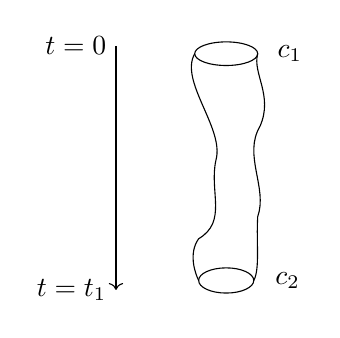
\begin{tikzpicture}[x=1cm,y=1cm]
\draw[->] (-1.4,3.1) -- (-1.4,0);
\node[left] at (-1.4,3.1) {$t=0$};
\node[left] at (-1.4,0) {$t=t_1$};
\draw (0,3) ellipse (0.40 and 0.15);
\draw (-0.40,3) .. controls (-0.60,2.65) and (-0.02,2.05) .. (-0.13,1.65) .. controls (-0.22,1.25) and (0.02,0.87) .. (-0.35,0.65) .. controls (-0.48,0.47) and (-0.40,0.22) .. (-0.35,0.12);
\draw (0.40,3) .. controls (0.33,2.75) and (0.60,2.47) .. (0.43,2.08) .. controls (0.21,1.71) and (0.53,1.30) .. (0.40,0.93) .. controls (0.38,0.60) and (0.43,0.27) .. (0.35,0.12);
\draw (0,0.12) ellipse (0.35 and 0.16);
\node[right] at (0.53,3) {$c_1$};
\node[right] at (0.50,0.12) {$c_2$};
\end{tikzpicture}
\end{adjustbox}
\begin{equation*}
(5)\qquad Z(c_1,c_2,t_1)\underset{t_1\to\infty}{=}\sum_nG(c_1,n)\,G(c_2,n)\,e^{-E_nt_1}.
\end{equation*}

Спектр стац. состояний в теории Лиувилля — спектр КТП для лагранжиана
[Над словами «теории Лиувилля» зачёркнуто: \Unclear{GELFAND-P001059}{liouville-cancellation}{неразборчивое слово}.]
\begin{equation*}
(6)\qquad\int_M\left[\frac12\partial_a\varphi\,\partial_a\varphi+m_0^2e^{\varphi}\right]d^2\xi.
\end{equation*}

\underline{Гипотеза}: спектр связан с системой $L_n$, опис. на предыд. странице.
\begin{gather*}
z=\xi_1+i\xi_2,\\
\bar z=\xi_1-i\xi_2.
\end{gather*}
Бесследный 2-мерный сохр. тензор эн.-импульса:
\begin{equation*}
T_{ab}=\partial_a\varphi\,\partial_b\varphi-\frac12\delta_{ab}(\partial_c\varphi)^2+\alpha\partial_a\partial_b\varphi-\beta\delta_{ab}(\partial_c\varphi)^2.
\end{equation*}
\Unclear{GELFAND-P001059}{tensor-last-term}{В последнем слагаемом записано $-\beta\delta_{ab}(\partial_c\varphi)^2$.}
\begin{align*}
T&=\varphi_z^2+2\varphi_{zz}, &\partial_{\bar z}T&=0,\\
\bar T&=\varphi_{\bar z}^2+2\varphi_{\bar z\bar z}, &\partial_zT&=0.
\end{align*}
[У первого $T$ зачёркнут нижний индекс: \Unclear{GELFAND-P001059}{tensor-cancelled-index}{$zz$?}.]
\Unclear{GELFAND-P001059}{lower-holomorphic}{Во втором равенстве справа записано $\partial_zT=0$; черта над $T$ не видна.}
\begin{equation*}
T(z)=\sum_{n=-\infty}^{\infty}z^{n-2}L_n
\qquad\text{— отсюда берутся }L_n!
\end{equation*}
[Под формулой скобка с подписью: «(разлаг. в ряд)».]

\SourcePage{GELFAND-P001060}{unlabelled}
% SOURCE {"image_path":"images/GELFAND-P001060.png","source_relative_path":"chapter_022/22_part_000035.png","sha256":"144e4a018beb5b17d99d5c010f3f9f5d90c0dd13839c62db0a54a5ba9aedcad5","width":2432,"height":3480}
% CATALOGUE {"academic_year":"1977-78","association_kind":"talk","catalogue_record_page":"record-573.html","catalogue_record_url":"https://old.mccme.ru/gelfand/notes/record-573.html","date_as_catalogued":"1982-11-01","label":"1-Nov-82, Al-dr.B. Zamolodchikov.","metadata_policy":"Preserved from source catalogue; association is not an exact in-image talk boundary.","record":573,"speaker_as_catalogued":"Al-dr.B. Zamolodchikov"}
% CATALOGUE {"academic_year":"1977-78","association_kind":"talk","catalogue_record_page":"record-574.html","catalogue_record_url":"https://old.mccme.ru/gelfand/notes/record-574.html","date_as_catalogued":"1982-11-01","label":"1-Nov-82, A.A. Beilinson.","metadata_policy":"Preserved from source catalogue; association is not an exact in-image talk boundary.","record":574,"speaker_as_catalogued":"A.A. Beilinson"}
% CATALOGUE {"academic_year":"1977-78","association_kind":"talk","catalogue_record_page":"record-575.html","catalogue_record_url":"https://old.mccme.ru/gelfand/notes/record-575.html","date_as_catalogued":"1982-11-15","label":"15-Nov-82, I.M. Gelfand.","metadata_policy":"Preserved from source catalogue; association is not an exact in-image talk boundary.","record":575,"speaker_as_catalogued":"I.M. Gelfand"}
% CATALOGUE {"academic_year":"1977-78","association_kind":"talk","catalogue_record_page":"record-576.html","catalogue_record_url":"https://old.mccme.ru/gelfand/notes/record-576.html","date_as_catalogued":"1982-11-15","label":"15-Nov-82, Yu.I. Manin.","metadata_policy":"Preserved from source catalogue; association is not an exact in-image talk boundary.","record":576,"speaker_as_catalogued":"Yu.I. Manin"}
% REVIEW {"page_id":"GELFAND-P001060","region_id":"heading","bbox":[170,30,2375,385],"magnification":3,"uncertainty_ids":[]}
% REVIEW {"page_id":"GELFAND-P001060","region_id":"theorem-top","bbox":[185,375,2430,795],"magnification":3,"uncertainty_ids":[]}
% REVIEW {"page_id":"GELFAND-P001060","region_id":"sheaf","bbox":[250,780,1960,1145],"magnification":3,"uncertainty_ids":[]}
% REVIEW {"page_id":"GELFAND-P001060","region_id":"theorem-bottom","bbox":[245,1140,2250,1670],"magnification":3,"uncertainty_ids":[]}
% REVIEW {"page_id":"GELFAND-P001060","region_id":"reference-year","bbox":[755,125,1140,220],"magnification":8,"uncertainty_ids":["GELFAND-0114-U210","GELFAND-0114-U211"]}
% REVIEW {"page_id":"GELFAND-P001060","region_id":"first-paragraph","bbox":[1190,125,2390,230],"magnification":3,"uncertainty_ids":[]}
% REVIEW {"page_id":"GELFAND-P001060","region_id":"pair-callout","bbox":[1770,435,2160,600],"magnification":5,"uncertainty_ids":[]}
% REVIEW {"page_id":"GELFAND-P001060","region_id":"gluing-cancellation","bbox":[1485,1045,1715,1145],"magnification":7,"uncertainty_ids":["GELFAND-0114-U212"]}
% REVIEW {"page_id":"GELFAND-P001060","region_id":"cancelled-heading","bbox":[325,1250,715,1370],"magnification":5,"uncertainty_ids":["GELFAND-0114-U213"]}
% REVIEW {"page_id":"GELFAND-P001060","region_id":"bottom-note","bbox":[1030,1560,1610,1680],"magnification":5,"uncertainty_ids":["GELFAND-0114-U214"]}
% REVIEW {"page_id":"GELFAND-P001060","region_id":"model-group","bbox":[820,270,1250,365],"magnification":5,"uncertainty_ids":[]}
% REVIEW {"page_id":"GELFAND-P001060","region_id":"projective-symbol","bbox":[340,382,442,485],"magnification":8,"uncertainty_ids":[]}
% REVIEW {"page_id":"GELFAND-P001060","region_id":"cancelled-equation","bbox":[325,1250,715,1370],"magnification":5,"uncertainty_ids":[]}
% REVIEW {"page_id":"GELFAND-P001060","region_id":"bibliographic","bbox":[755,125,1140,220],"magnification":5,"uncertainty_ids":[]}

\underline{Бейлинсон А.}

\underline{И.М.Г.} Гельфанд, Пономарёв
(\Unclear{GELFAND-P001060}{reference-leading-mark}{зачёркнутая помета} УМН, $\sim1968$ г.)
свед. опис. неразлож. предст. гр. Лоренца к задаче лин. алгебры.
[Под знаком $\sim$ низко написан \Unclear{GELFAND-P001060}{reference-lower-mark}{знак, похожий на $2$}.]

\underline{Б.} \underline{модельный пример.} — $\mathrm{SL}(2,\mathbb R)$

На $\mathbb P^1$ надо классиф. $D$-модули с особ. в фикс. $2^{\text{х}}$ точках.

\underline{Теорема 1.} катег. $D$-модулей в диске с фикс. особ. эквивалентна катег.
(лин. отобр.)
[Над «лин.» вписано: «пар».]
\begin{center}
\begin{adjustbox}{max width=\linewidth}
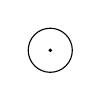
\begin{tikzpicture}[x=1cm,y=1cm]
\draw (0,0) circle (0.28);
\fill (0,0) circle (0.025);
\end{tikzpicture}
\end{adjustbox}
\hspace{1cm}
\begin{adjustbox}{max width=\linewidth}
\begin{tikzcd}
\Psi \arrow[r,shift left,"u"] & \Phi \arrow[l,shift left,"v"]
\end{tikzcd}
\end{adjustbox}
\end{center}
таких что $uv-\mathrm{Id}$ \underline{обратимо}.

[(вне $0$ — гладкие =\newline
= рассл. со связностью;\newline
в $0$ — регулярная особ.)]

\underline{Геом. задача.}
\begin{center}
\begin{adjustbox}{max width=\linewidth}
\begin{tikzcd}
Y \arrow[r,hook,"i"] & X & U=X\setminus Y \arrow[l,hook',"j"']
\end{tikzcd}
\end{adjustbox}
\end{center}
Пучок на $X$ зад. так:
\begin{equation*}
\mathcal{F}_X=(\mathcal{F}_U,\mathcal{F}_Y,\quad \mathcal{F}_Y\longrightarrow i^*j_*\mathcal{F}_U)
\end{equation*}
(ф-я [зачёркнуто: \Unclear{GELFAND-P001060}{gluing-cancellation}{неразборчивый фрагмент}] склейки)

Для представл. надо решить аналог. задачу на пр-ве флагов.

[Зачёркнуто: \Unclear{GELFAND-P001060}{cancelled-equation}{$Y=f^{-1}(0)$?}.]

\underline{Теор.} катег. $D$-мод. с регул. особ. на $X$ эквивал. катег. наборов
\begin{center}
$(M_U,M_Y,\quad$
\begin{adjustbox}{max width=\linewidth}
\begin{tikzcd}
M_Y \arrow[r,shift left,"v"] & \Psi(M_U) \arrow[l,shift left,"u"]
\end{tikzcd}
\end{adjustbox}
$)$
\end{center}
$vu=N$ — что-то.
[После «что-то.» зачёркнут \Unclear{GELFAND-P001060}{bottom-cancellation}{неразборчивый короткий знак}.]

\SourcePage{GELFAND-P001061}{48}
% SOURCE {"image_path":"images/GELFAND-P001061.png","source_relative_path":"chapter_022/22_part_000036.png","sha256":"e7155176b0e401fa3aa1b96d19df29f9e2898c0c547ab27b27e86f0bb956638f","width":2432,"height":3480}
% CATALOGUE {"academic_year":"1977-78","association_kind":"talk","catalogue_record_page":"record-573.html","catalogue_record_url":"https://old.mccme.ru/gelfand/notes/record-573.html","date_as_catalogued":"1982-11-01","label":"1-Nov-82, Al-dr.B. Zamolodchikov.","metadata_policy":"Preserved from source catalogue; association is not an exact in-image talk boundary.","record":573,"speaker_as_catalogued":"Al-dr.B. Zamolodchikov"}
% CATALOGUE {"academic_year":"1977-78","association_kind":"talk","catalogue_record_page":"record-574.html","catalogue_record_url":"https://old.mccme.ru/gelfand/notes/record-574.html","date_as_catalogued":"1982-11-01","label":"1-Nov-82, A.A. Beilinson.","metadata_policy":"Preserved from source catalogue; association is not an exact in-image talk boundary.","record":574,"speaker_as_catalogued":"A.A. Beilinson"}
% CATALOGUE {"academic_year":"1977-78","association_kind":"talk","catalogue_record_page":"record-575.html","catalogue_record_url":"https://old.mccme.ru/gelfand/notes/record-575.html","date_as_catalogued":"1982-11-15","label":"15-Nov-82, I.M. Gelfand.","metadata_policy":"Preserved from source catalogue; association is not an exact in-image talk boundary.","record":575,"speaker_as_catalogued":"I.M. Gelfand"}
% CATALOGUE {"academic_year":"1977-78","association_kind":"talk","catalogue_record_page":"record-576.html","catalogue_record_url":"https://old.mccme.ru/gelfand/notes/record-576.html","date_as_catalogued":"1982-11-15","label":"15-Nov-82, Yu.I. Manin.","metadata_policy":"Preserved from source catalogue; association is not an exact in-image talk boundary.","record":576,"speaker_as_catalogued":"Yu.I. Manin"}
% REVIEW {"page_id":"GELFAND-P001061","region_id":"heading-question","bbox":[140,50,2220,970],"magnification":3,"uncertainty_ids":[]}
% REVIEW {"page_id":"GELFAND-P001061","region_id":"agenda","bbox":[135,1120,2385,2335],"magnification":3,"uncertainty_ids":[]}
% REVIEW {"page_id":"GELFAND-P001061","region_id":"bottom-twistor","bbox":[140,2430,2360,3480],"magnification":3,"uncertainty_ids":[]}
% REVIEW {"page_id":"GELFAND-P001061","region_id":"questions-middle","bbox":[180,955,1320,1250],"magnification":3,"uncertainty_ids":[]}
% REVIEW {"page_id":"GELFAND-P001061","region_id":"top-definition","bbox":[360,265,2090,410],"magnification":3,"uncertainty_ids":[]}
% REVIEW {"page_id":"GELFAND-P001061","region_id":"top-cancelled-symbol","bbox":[215,275,400,405],"magnification":8,"uncertainty_ids":["GELFAND-0114-U220"]}
% REVIEW {"page_id":"GELFAND-P001061","region_id":"dimension-formula","bbox":[1570,485,2070,595],"magnification":7,"uncertainty_ids":[]}
% REVIEW {"page_id":"GELFAND-P001061","region_id":"hypothesis","bbox":[235,1115,1350,1250],"magnification":4,"uncertainty_ids":["GELFAND-0114-U222"]}
% REVIEW {"page_id":"GELFAND-P001061","region_id":"agenda-second","bbox":[230,1635,1640,1745],"magnification":3,"uncertainty_ids":[]}
% REVIEW {"page_id":"GELFAND-P001061","region_id":"involution","bbox":[595,2555,1435,2660],"magnification":5,"uncertainty_ids":["GELFAND-0114-U226"]}
% REVIEW {"page_id":"GELFAND-P001061","region_id":"three-cell-description","bbox":[190,2780,1620,2895],"magnification":3,"uncertainty_ids":["GELFAND-0114-U227"]}
% REVIEW {"page_id":"GELFAND-P001061","region_id":"plane-symbol","bbox":[550,3260,910,3420],"magnification":8,"uncertainty_ids":["GELFAND-0114-U228"]}
% REVIEW {"page_id":"GELFAND-P001061","region_id":"bottom-labels","bbox":[330,3275,585,3475],"magnification":8,"uncertainty_ids":[]}
% REVIEW {"page_id":"GELFAND-P001061","region_id":"question-leading-cancellation","bbox":[185,1235,270,1330],"magnification":10,"uncertainty_ids":["GELFAND-0114-U223"]}
% REVIEW {"page_id":"GELFAND-P001061","region_id":"agenda-cancelled-letter","bbox":[930,1620,1060,1730],"magnification":8,"uncertainty_ids":["GELFAND-0114-U224"]}
% REVIEW {"page_id":"GELFAND-P001061","region_id":"dimension-sum","bbox":[395,560,1055,695],"magnification":5,"uncertainty_ids":["GELFAND-0114-U221"]}
% REVIEW {"page_id":"GELFAND-P001061","region_id":"lower-involution-words","bbox":[610,2550,1060,2665],"magnification":8,"uncertainty_ids":["GELFAND-0114-U225"]}
% REVIEW {"page_id":"GELFAND-P001061","region_id":"schubert-coordinate-text","bbox":[290,380,1140,490],"magnification":4,"uncertainty_ids":[]}
% REVIEW {"page_id":"GELFAND-P001061","region_id":"agenda-item-two","bbox":[1040,1640,1630,1730],"magnification":5,"uncertainty_ids":[]}
% REVIEW {"page_id":"GELFAND-P001061","region_id":"agenda-footnote","bbox":[1020,2190,1980,2320],"magnification":4,"uncertainty_ids":[]}
% REVIEW {"page_id":"GELFAND-P001061","region_id":"schubert-initial-phrase","bbox":[260,365,1300,500],"magnification":4,"uncertainty_ids":["GELFAND-0114-U229"]}
% REVIEW {"page_id":"GELFAND-P001061","region_id":"involution-note","bbox":[595,2555,1435,2660],"magnification":5,"uncertainty_ids":[]}
% REVIEW {"page_id":"GELFAND-P001061","region_id":"three-cell-note","bbox":[190,2780,1620,2895],"magnification":3,"uncertainty_ids":[]}
% REVIEW {"page_id":"GELFAND-P001061","region_id":"schubert-text","bbox":[265,365,1220,500],"magnification":4,"uncertainty_ids":[]}

\underline{15/XI–82 г.}\qquad\underline{Сем. Гельфанда.}

\underline{И.М.Г.}\quad\underline{Задача} (неточная)

[В начале строки зачёркнуто: \Unclear{GELFAND-P001061}{top-cancelled-symbol}{$G$ с неразборчивыми приписанными знаками}.]
$G_{n,k}$ — грассм. мн-ие, $k$-мерн. плоск. в $n$-мерн. пр-ве.

\Unclear{GELFAND-P001061}{schubert-initial-phrase}{Когом. счит. / Коом. сист.} с пом. клеток Шуберта.

(Клетки зад. размерностями пересеч. с флагом
\begin{gather*}
0=d_0\le d_1\le d_2\le\ldots\le d_n=k,\\
\dim\text{ клетки}=\sum d_j.
\end{gather*}
)
\Unclear{GELFAND-P001061}{schubert-dimension}{В рукописи: $\dim\text{ клетки}=\sum d_j$.}

Рассм. $\mathrm{II}_1$-фактор; в нём рассм. $\alpha$-мерные проекторы (конт. аналог грассм. мн-ий).
\underline{Есть ли аналог клетки Шуберта?}

\underline{Флаг непр. размерности $[0,1]$.}

Получ. грассм. мн-ие?

Непр. когомологии!?

\underline{Гипотеза} [зачёркнуто: \Unclear{GELFAND-P001061}{hypothesis-cancellation}{неразборчивая короткая запись}]: описыв. монот. ф-ями.

[Перед «Ещё» зачёркнут \Unclear{GELFAND-P001061}{question-leading-cancellation}{неразборчивый знак}.]
Ещё более расплывчатый вопрос: какая топология? и какие когомологии?

\underline{Ю.И. Манин.}

1) Флаговые супермногообразия

2) Преобр. Радона–Пенроуза в [зачёркнут \Unclear{GELFAND-P001061}{agenda-cancelled-letter}{одиночный знак}] суперматем. ситуации.

3) Прилож. к решению нелин. ур-й: новые реш. неавтодуальных ур-й ЯМ
(обычные и суперсимм.)

4) Конкретные флаговые мн-ия, их искривление и т.п. в суперсимметрии и супергравитации.

5) Задача об индексе и о характеристич. классах.
[Под «об индексе»:]
(не сделана по настоящему)
[Под «о характеристич. классах»:]
(что-то важное сделал А.С. Шварц)

Будет об 1)–4)

1) \underline{Напоминание об автодуальных ур-ях Я.М.}

$T=\mathbb C^4$\qquad
[\Unclear{GELFAND-P001061}{involution-abbreviation}{антиголом. / антилин.} инвол. $T\oplus T^*$]
\Unclear{GELFAND-P001061}{involution-relation}{Между $T$ и $T^*$ записан знак $\oplus$.}

$\dim G(2,T)=4$ = комплексное компактное пр-во Минковского.

3-мерн. клетка (сем-во, параметр., \Unclear{GELFAND-P001061}{three-cell-description}{разл. / разн.} группой)

\begin{adjustbox}{max width=\linewidth}
\begin{tikzpicture}[x=1cm,y=1cm]
\node[left] at (-1.45,0) {$C^3(x)$};
\draw (-0.75,0.28) -- (0,0) -- (-0.75,-0.28);
\draw (-0.75,0) ellipse (0.11 and 0.28);
\draw (0.75,0.28) -- (0,0) -- (0.75,-0.28);
\draw (0.75,0) ellipse (0.11 and 0.28);
\fill (0,0) circle (0.025);
\node[below] at (0,-0.03) {$x$};
\node[right] at (1.8,0) {(опред. точкой).};
\node[left] at (-1.0,-0.95) {вершина конуса:};
\draw[->] (-0.9,-0.90) .. controls (-0.52,-0.88) and (-0.22,-0.62) .. (-0.12,-0.40);
\end{tikzpicture}
\end{adjustbox}

\begin{equation*}
M^4=\text{вещ. часть }G(2,T)\setminus C^3(\infty)\ \leftarrow\ \infty\text{-конус.}
\end{equation*}

2-мерн. клетки: 2 сорта

\Unclear{GELFAND-P001061}{plane-symbol}{$C^2_{\alpha,\beta}(x,\sigma^2\subset T_xM)$; знак $\sigma^2$ также может читаться как $a^2$}
— $\pm$-плоскости, $(\alpha,\beta)$-плоскости.

[Под индексом $\alpha$ стоит $+$, под индексом $\beta$ стоит $-$.]

\SourcePage{GELFAND-P001062}{unlabelled}
% SOURCE {"image_path":"images/GELFAND-P001062.png","source_relative_path":"chapter_022/22_part_000037.png","sha256":"7f54ca70601a5a06d3013af3f6082e42aca219e39785be5f7f9ae3917f70c6ba","width":2432,"height":3480}
% CATALOGUE {"academic_year":"1977-78","association_kind":"talk","catalogue_record_page":"record-574.html","catalogue_record_url":"https://old.mccme.ru/gelfand/notes/record-574.html","date_as_catalogued":"1982-11-01","label":"1-Nov-82, A.A. Beilinson.","metadata_policy":"Preserved from source catalogue; association is not an exact in-image talk boundary.","record":574,"speaker_as_catalogued":"A.A. Beilinson"}
% CATALOGUE {"academic_year":"1977-78","association_kind":"talk","catalogue_record_page":"record-575.html","catalogue_record_url":"https://old.mccme.ru/gelfand/notes/record-575.html","date_as_catalogued":"1982-11-15","label":"15-Nov-82, I.M. Gelfand.","metadata_policy":"Preserved from source catalogue; association is not an exact in-image talk boundary.","record":575,"speaker_as_catalogued":"I.M. Gelfand"}
% CATALOGUE {"academic_year":"1977-78","association_kind":"talk","catalogue_record_page":"record-576.html","catalogue_record_url":"https://old.mccme.ru/gelfand/notes/record-576.html","date_as_catalogued":"1982-11-15","label":"15-Nov-82, Yu.I. Manin.","metadata_policy":"Preserved from source catalogue; association is not an exact in-image talk boundary.","record":576,"speaker_as_catalogued":"Yu.I. Manin"}
% REVIEW {"page_id":"GELFAND-P001062","region_id":"top-diagram","bbox":[130,110,870,475],"magnification":3,"uncertainty_ids":[]}
% REVIEW {"page_id":"GELFAND-P001062","region_id":"problem","bbox":[250,525,2290,725],"magnification":3,"uncertainty_ids":[]}
% REVIEW {"page_id":"GELFAND-P001062","region_id":"flag","bbox":[230,805,2180,1000],"magnification":3,"uncertainty_ids":[]}
% REVIEW {"page_id":"GELFAND-P001062","region_id":"naive","bbox":[270,1220,2340,1535],"magnification":3,"uncertainty_ids":[]}
% REVIEW {"page_id":"GELFAND-P001062","region_id":"functor","bbox":[260,1520,1800,1910],"magnification":3,"uncertainty_ids":[]}
% REVIEW {"page_id":"GELFAND-P001062","region_id":"projective","bbox":[760,1900,2130,2045],"magnification":4,"uncertainty_ids":[]}
% REVIEW {"page_id":"GELFAND-P001062","region_id":"coordinates","bbox":[335,2100,2245,2400],"magnification":3,"uncertainty_ids":[]}
% REVIEW {"page_id":"GELFAND-P001062","region_id":"forms","bbox":[325,2460,2360,2910],"magnification":3,"uncertainty_ids":[]}
% REVIEW {"page_id":"GELFAND-P001062","region_id":"bottom","bbox":[235,2930,2345,3430],"magnification":3,"uncertainty_ids":[]}
% REVIEW {"page_id":"GELFAND-P001062","region_id":"first-line","bbox":[230,5,1300,140],"magnification":3,"uncertainty_ids":[]}
% REVIEW {"page_id":"GELFAND-P001062","region_id":"bundle-symbols","bbox":[380,110,855,320],"magnification":8,"uncertainty_ids":[]}
% REVIEW {"page_id":"GELFAND-P001062","region_id":"reduced-subscript","bbox":[1755,535,1945,635],"magnification":8,"uncertainty_ids":[]}
% REVIEW {"page_id":"GELFAND-P001062","region_id":"cancelled-flag","bbox":[640,815,750,950],"magnification":10,"uncertainty_ids":[]}
% REVIEW {"page_id":"GELFAND-P001062","region_id":"point-symbol","bbox":[2020,1905,2140,2040],"magnification":10,"uncertainty_ids":[]}
% REVIEW {"page_id":"GELFAND-P001062","region_id":"coordinate-last-index","bbox":[2030,2220,2220,2370],"magnification":10,"uncertainty_ids":[]}
% REVIEW {"page_id":"GELFAND-P001062","region_id":"forms-parenthesis","bbox":[1560,2675,2420,2825],"magnification":3,"uncertainty_ids":[]}
% REVIEW {"page_id":"GELFAND-P001062","region_id":"requirement","bbox":[535,3120,1680,3290],"magnification":4,"uncertainty_ids":[]}
% REVIEW {"page_id":"GELFAND-P001062","region_id":"cancelled-isotropic","bbox":[790,3260,1020,3400],"magnification":10,"uncertainty_ids":[]}
% REVIEW {"page_id":"GELFAND-P001062","region_id":"bundle-sketch","bbox":[130,110,870,475],"magnification":3,"uncertainty_ids":[]}

$C^1$ — нулевые прямые (лучи света)

\SourceFigure{GELFAND-P001062}{tautological-bundles}{Схема: над $G(2,T)$ стоит знак, похожий на $\xi$, $\zeta$ или рукописное $S$, от него стрелка вниз к $G(2,T)$. Справа вверху такой же знак с тильдой, затем $\subset T^*$; от правого знака стрелка по диагонали вниз-влево к $G(2,T)$. Под правым знаком стоят две короткие почти вертикальные черты и тот же знак со звёздочкой. Слева подпись «тавтол. рассл.», ниже «(2-комп. спиноры)»; от подписи стрелка вверх-вправо к левому верхнему знаку. Чтение самих обозначений расслоений и двух черт не установлено.}

\underline{Задача.} $G(2,T)$

Описать супероднородные компл. мн-зия $M$, для к-рых $M_{\mathrm{red}}=G(2,T)$.

Усл.: $M$ — флаговое мн-зие для простых супергрупп Ли классического типа.

\underline{Список} (начало).

\begin{equation*}
\text{а)}\quad F(2|0,2|N\ \text{[зачёркнут знак]},\mathbb C^{4|N})=M
\end{equation*}
\Unclear{GELFAND-P001062}{cancelled-flag-argument}{После $2|N$ зачёркнут знак, похожий на $2$.}
(флаги разм. $2|0,2|N$ в $\mathbb C^{4|N}$)
\begin{equation*}
N=0,1,2,3,\ldots
\end{equation*}
\begin{equation*}
\mathbb C^{4|N}=(\mathbb C^4)_0\oplus(\mathbb C^N)_1.
\end{equation*}
[Справа: «размерность $=4|4N$», с изогнутой стрелкой вверх к записи флагов.]

Наивное опред.:
\begin{equation*}
\text{точки }x\in F(2|0,2|N,\mathbb C^{4|N})
=\underline{\mathbb C^{2|0}\subset\mathbb C^{2|N}}\subset\mathbb C^{4|N}.
\end{equation*}
Но: нехватает координат.

Правильное опред.: $\forall$ суперкоммут. $\mathbb C$-алгебры $A$ задается $M(A)$
и тогда еще задается
\begin{equation*}
A\overset{f}{\longrightarrow}B.
\end{equation*}
\begin{adjustbox}{max width=\linewidth}
\begin{tikzcd}[column sep=small,row sep=large]
M(A)\arrow[d] & {:=N^{2|0}\subset N^{2|N}\subset A\otimes_{\mathbb C}\mathbb C^{4|N}}\\
M(B) & \text{(проективные)}\\
& \text{прямые подмодули}
\end{tikzcd}
\end{adjustbox}

\underline{Координаты:}
\begin{equation*}
G(1|0,\mathbb C^{m|n}):=P^{m-1|n}\ni\text{[неясный знак]}.
\end{equation*}
\Unclear{GELFAND-P001062}{projective-point-symbol}{После знака принадлежности: $\ell$ / $P$.}
Однородные коорд-ты: $(x_1,\ldots,x_m;\xi_1,\ldots,\xi_n)$.
\begin{equation*}
\text{Покрытие }P^{m-1,n}=\bigcup_{i=1}^{m}U_i,\qquad
U_i:\left(\frac{x_1}{x_i},\ldots,\frac{x_m}{x_i},\frac{\xi_1}{x_i},\ldots,\frac{\xi_m}{x_i}\right).
\end{equation*}
\Unclear{GELFAND-P001062}{affine-last-index}{Последняя аффинная координата на скане — $\xi_m/x_i$, хотя список однородных координат оканчивается $\xi_n$; возможная ошибка индекса сохранена буквально.}
Упражнение: связать с предыдущим (большие клетки).

Бывают: $\xi_i=0$ — клетка коразмерности $0|1$.

Неизвестно, в каких когомологиях они лежат?

Дифф. и интегр. форм тоже не хватает.
(они \Unclear{GELFAND-P001062}{forms-abbreviation}{«обслуж.»?} крайние разм.)

Шварцевские объекты промеж., но облад. странными св-вами.

Вещественные точки большой клетки в $F(2|0,2|N;\mathbb C^{4|N})=$
\begin{equation*}
=N\text{-расширенное }\underline{\text{суперпр-во физиков}}:
(x^m;\theta_{\alpha i},\theta^{\beta i}).
\end{equation*}
\underline{Требование:} [Над строкой, со знаком вставки: «сущ.»; зачёркнуто: «конформное».]
конформное пополнение.

\begin{equation*}
\text{б)}\quad FI(2|0,2|2,
\text{[зачёркнуты знаки]},
\mathbb C^{4|4},\Pi\mathrm{Sp})\qquad\text{Размерность}=4|8.
\end{equation*}
\Unclear{GELFAND-P001062}{cancelled-isotropic-argument}{Перед $\mathbb C^{4|4}$ зачёркнуто, возможно, $\mathrm{OSp}$.}

\SourcePage{GELFAND-P001063}{49}
% SOURCE {"image_path":"images/GELFAND-P001063.png","source_relative_path":"chapter_022/22_part_000038.png","sha256":"8564092a21de1188c22c332fb8409008ac5eda2f740fcdef2f6c217c742e143b","width":2432,"height":3480}
% CATALOGUE {"academic_year":"1977-78","association_kind":"talk","catalogue_record_page":"record-576.html","catalogue_record_url":"https://old.mccme.ru/gelfand/notes/record-576.html","date_as_catalogued":"1982-11-15","label":"15-Nov-82, Yu.I. Manin.","metadata_policy":"Preserved from source catalogue; association is not an exact in-image talk boundary.","record":576,"speaker_as_catalogued":"Yu.I. Manin"}
% CATALOGUE {"academic_year":"1977-78","association_kind":"talk","catalogue_record_page":"record-577.html","catalogue_record_url":"https://old.mccme.ru/gelfand/notes/record-577.html","date_as_catalogued":"1982-11-22","label":"22-Nov-82, A.M. Polyakov.","metadata_policy":"Preserved from source catalogue; association is not an exact in-image talk boundary.","record":577,"speaker_as_catalogued":"A.M. Polyakov"}
% REVIEW {"page_id":"GELFAND-P001063","region_id":"top","bbox":[190,75,2025,555],"magnification":3,"uncertainty_ids":[]}
% REVIEW {"page_id":"GELFAND-P001063","region_id":"cancelled-word","bbox":[210,265,410,355],"magnification":10,"uncertainty_ids":[]}
% REVIEW {"page_id":"GELFAND-P001063","region_id":"cancelled-word","bbox":[210,265,410,355],"magnification":6,"uncertainty_ids":[]}

$I$ — изотропные, $\Pi\mathrm{Sp}$ — тип формы, отн. к-рой флаги изотропны.

(нечетная симм. форма)

[Зачёркнуто: \Unclear{GELFAND-P001063}{cancelled-word}{«Бывают» / «Будут»}.]
Еще есть \underline{серии} и \underline{изолир.} мн-зия.

\begin{equation*}
2)\quad M=G(2,T),\qquad \underline{P(T)}=\underline{G(1,T)}.
\end{equation*}

\SourcePage{GELFAND-P001064}{unlabelled}
% SOURCE {"image_path":"images/GELFAND-P001064.png","source_relative_path":"chapter_022/22_part_000039.png","sha256":"84bdb9e8b2288e55b8f926b35bd9f5f3af3c7d170f7f89f721510ef62b5f7e20","width":2432,"height":3480}
% CATALOGUE {"academic_year":"1977-78","association_kind":"talk","catalogue_record_page":"record-576.html","catalogue_record_url":"https://old.mccme.ru/gelfand/notes/record-576.html","date_as_catalogued":"1982-11-15","label":"15-Nov-82, Yu.I. Manin.","metadata_policy":"Preserved from source catalogue; association is not an exact in-image talk boundary.","record":576,"speaker_as_catalogued":"Yu.I. Manin"}
% CATALOGUE {"academic_year":"1977-78","association_kind":"talk","catalogue_record_page":"record-577.html","catalogue_record_url":"https://old.mccme.ru/gelfand/notes/record-577.html","date_as_catalogued":"1982-11-22","label":"22-Nov-82, A.M. Polyakov.","metadata_policy":"Preserved from source catalogue; association is not an exact in-image talk boundary.","record":577,"speaker_as_catalogued":"A.M. Polyakov"}
% REVIEW {"page_id":"GELFAND-P001064","region_id":"heading","bbox":[100,1570,1220,1855],"magnification":3,"uncertainty_ids":[]}
% REVIEW {"page_id":"GELFAND-P001064","region_id":"intro","bbox":[150,1810,2110,2120],"magnification":3,"uncertainty_ids":[]}
% REVIEW {"page_id":"GELFAND-P001064","region_id":"equations","bbox":[180,2160,2250,2560],"magnification":3,"uncertainty_ids":[]}
% REVIEW {"page_id":"GELFAND-P001064","region_id":"bottom","bbox":[230,2580,2430,3140],"magnification":3,"uncertainty_ids":[]}
% REVIEW {"page_id":"GELFAND-P001064","region_id":"final-text","bbox":[65,3110,2425,3475],"magnification":3,"uncertainty_ids":[]}
% REVIEW {"page_id":"GELFAND-P001064","region_id":"sphere-caption","bbox":[660,1890,1340,2050],"magnification":3,"uncertainty_ids":[]}
% REVIEW {"page_id":"GELFAND-P001064","region_id":"liouville-symbol","bbox":[1920,3280,2040,3410],"magnification":10,"uncertainty_ids":[]}
% REVIEW {"page_id":"GELFAND-P001064","region_id":"metric-caption","bbox":[730,2150,1730,2260],"magnification":3,"uncertainty_ids":[]}
% REVIEW {"page_id":"GELFAND-P001064","region_id":"form-three","bbox":[120,2515,2390,2740],"magnification":3,"uncertainty_ids":[]}
% REVIEW {"page_id":"GELFAND-P001064","region_id":"sphere-caption","bbox":[860,1900,1330,2010],"magnification":3,"uncertainty_ids":[]}

\underline{22/XI-82 г.}\qquad \underline{\underline{Сем. Гельфанда.}}

\underline{\underline{А. М. Поляков.}}

(Ал-др Маркович).

Зад. о струне
\begin{adjustbox}{max width=\linewidth}
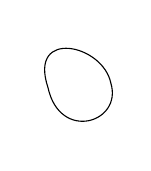
\begin{tikzpicture}
\draw (0.1,0.6) .. controls (-0.15,1.35) and (0.8,1.15) .. (0.9,0.65)
.. controls (1.05,0.15) and (0.25,-0.1) .. (0.1,0.6);
\end{tikzpicture}
\end{adjustbox}
— \Unclear{GELFAND-P001064}{string-caption}{«нем. возбуд.» / «геом. возбуд.»}

Сводится к следующему: есть поле
\begin{equation*}
\varphi=\varphi(\xi_1,\xi_2)\qquad (\sim\text{ пов. в изотермич. коорд.})
\end{equation*}
\begin{equation*}
g_{ab}(\xi)=e^{\varphi(\xi)}\delta_{ab}.\tag{1}
\end{equation*}
\begin{equation*}
\mathcal L=\frac1\gamma\left\{\frac12(\partial_a\varphi)^2+e^\varphi\right\},
\qquad S=\int\mathcal L\,d^2\xi,\tag{2}
\end{equation*}
\begin{equation*}
\frac1\gamma=\frac{26-D}{48\pi}\tag{3}
\end{equation*}
($D$ — разм. пр-ва, в к-рое вклад. рассм. 2-мерная пов.)

Откуда вид (2) (кроме $\gamma$)?

Фиксир. метрику (1). Остаток свободы: конформные преобр.
\begin{equation*}
e^{\widetilde\varphi(z,\bar z)}
=\left|\frac{dw}{dz}\right|^2e^{\varphi(w(z),\bar w(z))}.\tag{4}
\end{equation*}
\Unclear{GELFAND-P001064}{conformal-last-argument}{В правом показателе (4) написано $\varphi(w(z),\bar w(z))$: черта видна над вторым $w$, но не над последним $z$. Возможная ошибка источника сохранена буквально.}
Лагр. (2) — единств. лок. лагранжиан (завис. лишь от знач. ф-и и ее произв.
в точке), не меняющийся при преобр. (4).

$\mathcal L$ наз. \underline{лагранжианом Лиувилля}
(соотв. ур-е $\Delta\varphi=e^\varphi$
\Unclear{GELFAND-P001064}{liouville-cancelled-symbol}{[После $e^\varphi$ перечёркнут скобкообразный знак.]}
или $\partial^2\varphi=e^\varphi$).

\SourcePage{GELFAND-P001065}{unlabelled}
% SOURCE {"image_path":"images/GELFAND-P001065.png","source_relative_path":"chapter_022/22_part_000040.png","sha256":"926f8f784d36456cacf62725caa2e72dd2f904e458d1d1283ee95f51d9fca100","width":2432,"height":3480}
% CATALOGUE {"academic_year":"1977-78","association_kind":"talk","catalogue_record_page":"record-576.html","catalogue_record_url":"https://old.mccme.ru/gelfand/notes/record-576.html","date_as_catalogued":"1982-11-15","label":"15-Nov-82, Yu.I. Manin.","metadata_policy":"Preserved from source catalogue; association is not an exact in-image talk boundary.","record":576,"speaker_as_catalogued":"Yu.I. Manin"}
% CATALOGUE {"academic_year":"1977-78","association_kind":"talk","catalogue_record_page":"record-577.html","catalogue_record_url":"https://old.mccme.ru/gelfand/notes/record-577.html","date_as_catalogued":"1982-11-22","label":"22-Nov-82, A.M. Polyakov.","metadata_policy":"Preserved from source catalogue; association is not an exact in-image talk boundary.","record":577,"speaker_as_catalogued":"A.M. Polyakov"}
% REVIEW {"page_id":"GELFAND-P001065","region_id":"independent-schwarzian","bbox":[1270,2050,1870,2280],"magnification":6,"uncertainty_ids":[]}
% REVIEW {"page_id":"GELFAND-P001065","region_id":"independent-stress-derivatives","bbox":[350,1760,1025,1910],"magnification":6,"uncertainty_ids":[]}
% REVIEW {"page_id":"GELFAND-P001065","region_id":"independent-final-reference","bbox":[1070,2950,2190,3140],"magnification":4,"uncertainty_ids":[]}
% REVIEW {"page_id":"GELFAND-P001065","region_id":"top","bbox":[250,50,2370,535],"magnification":3,"uncertainty_ids":[]}
% REVIEW {"page_id":"GELFAND-P001065","region_id":"middle","bbox":[360,1750,2200,2420],"magnification":3,"uncertainty_ids":[]}
% REVIEW {"page_id":"GELFAND-P001065","region_id":"bottom","bbox":[380,2510,2390,3410],"magnification":3,"uncertainty_ids":[]}
% REVIEW {"page_id":"GELFAND-P001065","region_id":"schwarzian","bbox":[1270,2070,1900,2250],"magnification":6,"uncertainty_ids":[]}
% REVIEW {"page_id":"GELFAND-P001065","region_id":"equations-bottom","bbox":[400,2690,2350,3420],"magnification":3,"uncertainty_ids":[]}
% REVIEW {"page_id":"GELFAND-P001065","region_id":"sphere-diagram","bbox":[45,390,785,1130],"magnification":3,"uncertainty_ids":[]}
% REVIEW {"page_id":"GELFAND-P001065","region_id":"cusp-asymptotic","bbox":[590,555,2290,1040],"magnification":3,"uncertainty_ids":[]}
% REVIEW {"page_id":"GELFAND-P001065","region_id":"path-integral","bbox":[285,1040,2390,1390],"magnification":3,"uncertainty_ids":[]}
% REVIEW {"page_id":"GELFAND-P001065","region_id":"uniformization","bbox":[275,1400,2375,1760],"magnification":3,"uncertainty_ids":[]}
% REVIEW {"page_id":"GELFAND-P001065","region_id":"monodromy-text","bbox":[435,2790,2380,3070],"magnification":3,"uncertainty_ids":[]}
% REVIEW {"page_id":"GELFAND-P001065","region_id":"final-lines","bbox":[345,3090,2350,3445],"magnification":3,"uncertainty_ids":[]}
% REVIEW {"page_id":"GELFAND-P001065","region_id":"cancelled-pole","bbox":[1580,2675,1915,2830],"magnification":10,"uncertainty_ids":[]}
% REVIEW {"page_id":"GELFAND-P001065","region_id":"uniformization-caption","bbox":[1800,1435,2280,1555],"magnification":5,"uncertainty_ids":[]}
% REVIEW {"page_id":"GELFAND-P001065","region_id":"sphere-full","bbox":[120,415,955,1260],"magnification":3,"uncertainty_ids":[]}
% REVIEW {"page_id":"GELFAND-P001065","region_id":"small-insertion","bbox":[685,2790,1925,2895],"magnification":4,"uncertainty_ids":[]}
% REVIEW {"page_id":"GELFAND-P001065","region_id":"cancelled-before-ode","bbox":[340,2840,800,2945],"magnification":6,"uncertainty_ids":[]}
% REVIEW {"page_id":"GELFAND-P001065","region_id":"diagram-eight","bbox":[585,1245,1580,1600],"magnification":3,"uncertainty_ids":[]}
% REVIEW {"page_id":"GELFAND-P001065","region_id":"accessory-word","bbox":[1965,2835,2355,2920],"magnification":6,"uncertainty_ids":[]}
% REVIEW {"page_id":"GELFAND-P001065","region_id":"important-line","bbox":[395,2730,2390,2860],"magnification":3,"uncertainty_ids":[]}
% REVIEW {"page_id":"GELFAND-P001065","region_id":"real-field","bbox":[2070,3235,2135,3325],"magnification":10,"uncertainty_ids":[]}
% REVIEW {"page_id":"GELFAND-P001065","region_id":"complex-field","bbox":[2080,3320,2165,3410],"magnification":10,"uncertainty_ids":[]}
% REVIEW {"page_id":"GELFAND-P001065","region_id":"equation-thirteen-comment","bbox":[1070,2950,2190,3140],"magnification":3,"uncertainty_ids":[]}
% REVIEW {"page_id":"GELFAND-P001065","region_id":"equation-thirteen-reference","bbox":[1960,2970,2180,3125],"magnification":10,"uncertainty_ids":[]}
% REVIEW {"page_id":"GELFAND-P001065","region_id":"schwarzian","bbox":[1300,2080,1860,2250],"magnification":6,"uncertainty_ids":[]}
% REVIEW {"page_id":"GELFAND-P001065","region_id":"uniformization-caption","bbox":[1800,1435,2280,1555],"magnification":5,"uncertainty_ids":[]}

\begin{equation*}
\partial^2\varphi\equiv\Delta\varphi=e^\varphi.\tag{5}
\end{equation*}
\underline{Явно решается.} ($\sim$ кривизна постоянна)

Классическое решение ур-я (5):
\begin{equation*}
\varphi=\log\left(\frac{|\partial_z w|^2}{(\operatorname{Im}w)^2}\right),
\qquad w(z)\text{ — любая аналит. ф-я}.\tag{6}
\end{equation*}

\begin{adjustbox}{max width=\linewidth}
\begin{tikzpicture}[scale=0.9]
\draw (-1.4,2.1) .. controls (-1.05,1.6) and (-0.65,1.3) .. (-0.35,0.75)
.. controls (-0.1,0.95) and (0.35,0.9) .. (0.5,0.72)
.. controls (1.0,0.97) and (1.65,1.6) .. (2.3,1.85)
.. controls (1.85,1.35) and (1.4,0.95) .. (0.72,0.45)
.. controls (0.85,0.15) and (0.75,-0.15) .. (0.63,-0.3)
.. controls (1.35,-0.4) and (2.3,-1.1) .. (3.05,-1.75)
.. controls (2.2,-1.45) and (1.2,-1.1) .. (0.38,-1.0)
.. controls (0.16,-1.24) and (-0.3,-1.2) .. (-0.54,-1.02)
.. controls (-1.05,-1.55) and (-1.8,-2.5) .. (-2.45,-3.2)
.. controls (-1.93,-2.31) and (-1.17,-1.56) .. (-0.84,-0.9)
.. controls (-1.12,-0.63) and (-1.05,0.07) .. (-0.72,0.35)
.. controls (-1.05,0.65) and (-1.11,1.55) .. (-1.4,2.1);
\node[above right] at (-1.4,2.1) {$z_1$};
\node[right] at (2.3,1.85) {$z_2$};
\node[below right] at (-2.45,-3.2) {$z_N$};
\end{tikzpicture}
\end{adjustbox}

Рассм. сферу с выкол. точками, к-рые на $\infty$ в смысле метрики.
\begin{equation*}
e^\varphi\underset{z\to z_i}{\longrightarrow}
\frac{2}{|z-z_i|^2\log^2|z-z_i|}.
\end{equation*}
хотим выч. квантовую велич.
\begin{equation*}
\Psi(z_1,\ldots,z_N)=\int\mathcal D\varphi(z)e^{-S(\varphi)}
\underset{\gamma\to0}{\simeq}e^{-S_{\mathrm{cl}}(z_1,\ldots,z_N)}.\tag{7}
\end{equation*}
Вычислим $S_{\mathrm{cl}}$.

(8)
\begin{adjustbox}{max width=\linewidth}
\begin{tikzpicture}
\draw (0,0.4) circle (0.025);
\fill (0.55,0.62) circle (0.025);
\fill (1.25,0.42) circle (0.025);
\draw (1.67,0.57) circle (0.022);
\draw (0.94,0.06) circle (0.025);
\draw (0.59,-0.23) circle (0.025);
\node at (2.7,0.12) {$\Rightarrow$};
\node[above] at (4.5,1.43) {$[z_1,\ldots,z_N]$};
\draw (3.65,-0.22)--(6.9,-0.29);
\draw (4.18,1.12)--(4.03,-0.16)
.. controls (4.14,0.62) and (4.57,0.54) .. (4.58,-0.14)
.. controls (4.83,0.70) and (5.25,0.66) .. (5.25,-0.14)
.. controls (5.52,0.65) and (5.9,0.61) .. (5.9,-0.12)
.. controls (6.21,0.43) and (6.54,0.45) .. (6.55,-0.22)
--(6.91,1.28);
\draw (3.71,-0.65)--(4.05,-0.28);
\draw (4.03,-0.72)--(4.5,-0.29);
\draw (4.49,-0.78)--(5.02,-0.34);
\draw (4.97,-0.75)--(5.65,-0.37);
\draw (5.45,-0.76)--(6.18,-0.38);
\draw (5.98,-0.76)--(6.62,-0.38);
\draw (6.3,-0.83)--(6.85,-0.41);
\draw (6.58,-0.78)--(6.99,-0.44);
\draw (6.84,-0.76)--(7.13,-0.5);
\node[below] at (5.57,-1.0) {$(0\text{-е усл.})$};
\end{tikzpicture}
\end{adjustbox}
(накрывающая)

Вычислим тензор эн.-импульса:
\begin{equation*}
T=\frac12(\partial_z\varphi)^2-\partial_z^2\varphi,
\qquad T=T_{11}-T_{22}+2iT_{12},\qquad T_{11}+T_{22}=0.\tag{9}
\end{equation*}
($T_{ij}$ восстан. по $T$, т.к. $T_{ij}$ — вещ.)

\begin{equation*}
T(z|z_1,\ldots,z_N)=\mathcal D[w(z)]
=\frac{w'''}{w'^2}-\frac32\frac{(w'')^2}{(w')^4}.\tag{10}
\end{equation*}
[Под $\mathcal D$: «(произв. Шварца)».]
\Unclear{GELFAND-P001065}{schwarzian-denominators}{В (10) знаменатели на скане читаются $w'^2$ и $(w')^4$; возможная ошибка источника сохранена без исправления.}

(инвар. отн. дробно-лин. преобр.)
\begin{equation*}
\widetilde w(z)=\frac{\alpha w+\beta}{\gamma w+\delta}.
\end{equation*}
Отсюда $T$ — однозначна и имеет лишь полюса:
\begin{equation*}
T(z|z_1,\ldots,z_N)=\frac14\sum_1^N\frac1{(z-z_i)^2}
+\sum_1^N\frac{c_i(z_1,\ldots,z_N)}{z-z_i}.\tag{11}
\end{equation*}
\Unclear{GELFAND-P001065}{cancelled-pole-denominator}{В знаменателе последней дроби перед $z-z_i$ густо перечёркнуты один-два знака; чтение не установлено.}

Важно, чтобы $c_i$ были вещественны и этим $c_i$ фиксируются.

($c_i$ — акцессорные коэффициенты)

[Мелко над строкой (12):] Это связ. с веществ. коэф. монодромии ур-я:

[Перед формулой (12) зачёркнуто: \Unclear{GELFAND-P001065}{cancelled-before-ode}{«(Это видно)» / «(Это важно)»}.]
\begin{equation*}
\psi''+T(z)\psi=0.\tag{12}
\end{equation*}
\begin{equation*}
w(z)=\frac{\psi_1(z)}{\psi_2(z)}.\tag{13}
\end{equation*}
($\psi_1,\psi_2$ — 2 лин. незав. реш. (13))
\Unclear{GELFAND-P001065}{solution-equation-reference}{В пояснении к (13) на скане стоит «реш. (13)», хотя дифференциальное уравнение выше обозначено (12); ссылка источника оставлена без исправления.}

\underline{Условие на вар. $c$:} монодромия меняется, но остается веществ.,

(в этом сост. задача)

(в $SL(2,\mathbb R)$, а не в $SL(2,\mathbb C)$)

\SourcePage{GELFAND-P001066}{55}
% Full original scan frame inspected; manuscript regions read top-to-bottom.
% Review crops: original-pixel bbox [x0,y0,x1,y1), origin top left; nearest-neighbour scale.
% REVIEW top bbox=[48, 0, 2399, 950] scale=3.0x
% REVIEW middle bbox=[71, 914, 2197, 1876] scale=3.0x
% REVIEW lower-math bbox=[59, 1864, 2399, 2684] scale=3.0x
% REVIEW bottom bbox=[59, 2636, 2351, 3444] scale=3.0x
% REVIEW quasi-symbol bbox=[1986, 259, 2218, 378] scale=10.0x
% REVIEW top-word bbox=[242, 45, 401, 145] scale=5.0x
% REVIEW correction-15 bbox=[549, 368, 734, 506] scale=6.0x
% REVIEW crossed-15 bbox=[366, 530, 468, 634] scale=8.0x
% REVIEW bracket-17 bbox=[907, 1470, 1047, 1598] scale=8.0x
Связь:
\begin{equation*}
c_i(z_1,\ldots,z_N)=\frac{\partial S_{cl}}{\partial z_i}.
\tag{14}
\end{equation*}
Решение зад. через квантовую и затем квазиклассика при \Unclear{GELFAND-P001066}{quasiclassical-parameter}{$\gamma$ / $\delta$ / $\hbar$} $\to0$!
\begin{equation*}
[T(z_1),T(z_2)]=(T(z_1)+T(z_2))\delta'(z_1-z_2)+\frac{c}{12}\delta'''(z_1-z_2).
\tag{15}
\end{equation*}
[Правка: \Unclear{GELFAND-P001066}{eq15-superscript-correction}{над $z_2$ зачёркнут знак: $1$ / $2$?}.]
[\Unclear{GELFAND-P001066}{eq15-crossed-mark}{заштрихованный знак неразборчив}.]
(завис. от $z_1,\ldots,z_N$ не пишем)

или:
\begin{equation*}
[T(z),T(w)]=(T(z)+T(w))\delta'(z-w)+\frac{c}{12}\delta'''(z-w)
\tag{15}
\end{equation*}
(в классике. скобки Пуассона)

Считаем:

Лагранжиан:
\begin{equation*}
\mathcal{L}=\int\bigl(\partial_z\varphi\,\partial_{\bar z}\varphi-e^{\varphi}\bigr)
\end{equation*}
\begin{equation*}
p=\frac{\partial\mathcal{L}}{\partial(\partial_{\bar z}\varphi)}=\partial_z\varphi
\tag{16}
\end{equation*}
[На правом поле: Вирасоро.]

откуда
\begin{equation*}
\{\varphi(z),\partial_w\varphi(w)\}=\text{[неясный штрих]}\delta(z-w).
\tag{17}
\end{equation*}
[\Unclear{GELFAND-P001066}{eq17-before-delta}{перед $\delta$: отдельный множитель $\gamma$ или штрих правки?}]
$\{T(z),T(w)\}$ и т. д.

Разлагаем в ряд Лорана:
\begin{equation*}
T(z)=\sum_n(L_nz^n+L_{-n}z^{-n})
\tag{18}
\end{equation*}
\begin{equation*}
[L_n,L_m]=(n-m)L_{n+m}+\frac{c}{12}n(n^2-1),\quad c=26-D.
\tag{19}
\end{equation*}
[\Unclear{GELFAND-P001066}{eq19-central-term}{в центральном слагаемом (19) множитель с $\delta$ не написан}]
(можно было предсказать из рез. Гельфанда-Фукса из вида центр. расш.)
\begin{equation*}
\widetilde z=z+\varepsilon(z)\qquad\text{(вариация)}
\end{equation*}
\begin{equation*}
\delta\varphi=\operatorname{Re}(\varepsilon(z)\partial_z\varphi+\partial_z\varepsilon)
\end{equation*}
К действию доб. число $\rightsquigarrow$ появл. центр. расширение).

Попробуем найти $\Psi$ чисто алгебраически:
\begin{equation*}
\text{Пусть}\qquad T_{\varepsilon}=\int\varepsilon(z)T(z)\,d^2z
\tag{20}
\end{equation*}
[Справа, со стрелкой влево к формулам: Предположим, что генератор сдвига.]
\begin{equation*}
\delta_{\varepsilon}\psi=[T_{\varepsilon},\psi(z)]
=\varepsilon(z)\frac{d\psi}{dz}+\Delta\cdot\varepsilon'(z)\psi(z)
\tag{21}
\end{equation*}
(вариация поля $\psi$)
\begin{equation*}
[L_n,\psi(z)]=z^{n+1}\frac{d\psi}{dz}+(n+1)\Delta\psi(z).
\tag{22}
\end{equation*}
[\Unclear{GELFAND-P001066}{eq22-weight-term}{во втором слагаемом (22) $z^n$ не написано}]
$\psi(z)$ — опер. в том же пр-ве, где задано представление.

\SourcePage{GELFAND-P001067}{unlabelled}
% Full original scan frame inspected; manuscript regions read top-to-bottom.
% Review crops: original-pixel bbox [x0,y0,x1,y1), origin top left; nearest-neighbour scale.
% REVIEW top bbox=[95, 24, 2185, 1271] scale=3.0x
% REVIEW middle bbox=[142, 1259, 2339, 2244] scale=3.0x
% REVIEW bottom bbox=[356, 2244, 2387, 3444] scale=3.0x
% REVIEW heading-mark bbox=[546, 1608, 694, 1734] scale=6.0x
% REVIEW overwritten-field bbox=[366, 1385, 506, 1508] scale=6.0x
% REVIEW corrected-factor bbox=[860, 2610, 1074, 2769] scale=7.0x
% REVIEW action-subscript bbox=[1416, 2997, 1653, 3133] scale=8.0x
% REVIEW last-line bbox=[499, 3225, 1698, 3408] scale=4.0x
$\psi(z)$ — опер. рожд. рога на сфере.
\begin{equation*}
\psi(z)|v\rangle.
\end{equation*}
Рассм. ф-и:
\begin{equation*}
\langle v|\psi(z_1)\psi(z_2)\psi(z_3)\psi(z_4)|v\rangle
\tag{23}
\end{equation*}
\begin{equation*}
\Psi(x)=\langle v|\psi(\infty)\psi(1)\psi(x)\psi(0)|v\rangle
\end{equation*}
\begin{equation*}
|0\rangle=\psi(0)|v\rangle,\qquad \langle v|\psi(\infty)=\langle0|
\end{equation*}
\begin{equation*}
\Psi(x)=\langle0|\psi(1)\psi(x)|0\rangle
\end{equation*}
\begin{equation*}
\begin{cases}
L_n|0\rangle=0,\quad n>0,\\
L_0|0\rangle=\Delta|0\rangle
\end{cases}
\tag{24}
\end{equation*}
Возникают модули Верма: такое предст. без лишних соотн.

\Unclear{GELFAND-P001067}{overwritten-field}{$\psi(x)$ / $\Psi(x)$} опис. выше и перев. мод. Верма в себя.
\begin{equation*}
\Psi(x)=e^{\Delta\cdot S_{cl}(x)}\quad\Rightarrow\quad\text{по }\Psi(x)\text{ всё опред.}
\tag{25}
\end{equation*}
\Unclear{GELFAND-P001067}{heading-mark}{§. / 4. / зачёркнутый знак} \underline{Вычисление $\Psi$.}

Добавим соотношение (к коммут. соотн.):
\begin{equation*}
\langle0|\psi(x)|0\rangle=x^{-\Delta}
\tag{26}
\end{equation*}
\begin{equation*}
\begin{aligned}
&\langle0|\psi(1)|0\rangle\langle0|\psi(x)|0\rangle+
\langle0|\psi(1)|1\rangle\langle1|\psi(x)|0\rangle+\\
&\quad+\langle0|\psi(1)|2\rangle\langle2|\psi(x)|0\rangle+\ldots
\end{aligned}
\tag{27}
\end{equation*}
\begin{equation*}
I=\sum_n|n\rangle\langle n|
\end{equation*}
\begin{equation*}
\begin{aligned}
\langle1|\psi(x)|0\rangle
&=\langle0|L_1\psi(x)|0\rangle
=\langle0|[L_1,\psi(x)]|0\rangle=\\
&=\left(x^2\frac{d}{dx}+2\Delta x\right)\langle0|\psi(x)|0\rangle
=(\Delta\cdot x)x^{-\Delta}
\end{aligned}
\end{equation*}
[Правка: \Unclear{GELFAND-P001067}{matrix-element-correction}{после $2\Delta$ зачёркнуто $\psi$ / $\varphi$?; вписано $x$; нижний крючок: вставка / $y$}.]

и далее получается:
\begin{equation*}
\Psi(x)=x^{-\Delta}\left\{1+\frac{\Delta}{2}x+\ldots\right\}
\end{equation*}
\begin{equation*}
\langle v|\psi(z_1)\ldots\psi(z_N)|v\rangle=e^{-S_{ii}(z_1,\ldots,z_N)}
\end{equation*}
[\Unclear{GELFAND-P001067}{action-subscript}{нижний индекс у $S$: $ii$ / $li$ / $cl$}]
\begin{equation*}
\Delta,c\to\infty
\end{equation*}
$c_i(z_1,\ldots,z_N)$ при $z_i-z_j\to0$ [\Unclear{GELFAND-P001067}{last-line-cancellation}{при / пре; зачёркнуто}] перех. в предыдущий акцессорный коэффициент?

\SourcePage{GELFAND-P001068}{56}
% Full original scan frame inspected; manuscript regions read top-to-bottom.
% Review crops: original-pixel bbox [x0,y0,x1,y1), origin top left; nearest-neighbour scale.
% REVIEW top bbox=[154, 19, 2356, 922] scale=3.0x
% REVIEW middle bbox=[154, 886, 2173, 1879] scale=3.0x
% REVIEW lower bbox=[190, 1829, 2197, 2848] scale=3.0x
% REVIEW bottom bbox=[238, 2826, 2104, 3396] scale=3.0x
% REVIEW deleted-word bbox=[290, 228, 594, 321] scale=5.0x
% REVIEW deleted-exponent bbox=[625, 553, 712, 648] scale=9.0x
% REVIEW deleted-after-psi bbox=[1164, 1484, 1275, 1584] scale=8.0x
% REVIEW basis-text bbox=[285, 2465, 881, 2586] scale=5.0x
% REVIEW deleted-basis bbox=[841, 2627, 933, 2726] scale=8.0x
% REVIEW natural-text bbox=[166, 1753, 1235, 1900] scale=4.0x
% REVIEW basis-abbreviation bbox=[1014, 2974, 1313, 3104] scale=5.0x
$S_{cl}(x)$

(3 другие точки $0,1,\infty$)

[Зачёркнуто: Остальные.] $\Rightarrow c_k=c_k(x)$
\begin{equation*}
c_k(x)=\frac{\partial S_{cl}(x)}{\partial x}
\end{equation*}
\begin{equation*}
e^{S_{cl}(x)}=x^{-\Delta}\{1+a_1x+a_2x^2+\ldots\}.
\end{equation*}
[\Unclear{GELFAND-P001068}{exponent-cancelled-mark}{знак после $S_{cl}(x)$ заштрихован, неразборчив}]
\underline{коэфф. $a_j$ вычисл. с пом. алгебры.}

Аксиомы:
\begin{equation*}
L_0|0\rangle=\Delta|0\rangle
\end{equation*}
\begin{equation*}
L_n|0\rangle=0,\quad n>0
\end{equation*}
\begin{equation*}
[L_n,\psi(x)]=\left(x^{n+1}\frac{d}{dx}+(n+1)\Delta\right)\psi(x)
\end{equation*}
[\Unclear{GELFAND-P001068}{axiom-commutator}{множитель $x^n$ при $(n+1)\Delta$ не написан}]
\begin{equation*}
\langle0|\psi(x)|0\rangle=x^{-\Delta}
\end{equation*}
\begin{equation*}
\Psi(x)=\langle0|\psi(1)\psi(x)|0\rangle
\end{equation*}
[\Unclear{GELFAND-P001068}{correlator-end-mark}{заштрихованный знак после $|0
angle$ неразборчив}]
\begin{equation*}
I=\sum_n|n\rangle\langle n|,\qquad |n\rangle=L_{-n}|0\rangle.
\end{equation*}
[На левом поле: $\psi(x)$ — ?]

Сложность. нет ортогональности.

Из вида $T$ естественно:
\begin{equation*}
L_n=(\alpha+i\beta n)a_n+\sum_{k=1}^{n-1}a_ka_{n-k}+\sum_{k=1}^{\infty}a_k^+a_{n+k};
\end{equation*}
\begin{equation*}
L_{-n}=L_n^+;
\end{equation*}
\begin{equation*}
[a_n,a_m^+]=n\delta_{n,m};
\end{equation*}
\begin{equation*}
\Delta=\frac12(\alpha^2+\beta^2),\quad c=1+12\beta^2.
\end{equation*}
\begin{equation*}
a_n|0\rangle=0.
\end{equation*}
Есть соотв. базисов:
\begin{equation*}
a_{n_1}^+a_{n_2}^+\ldots|0\rangle
\end{equation*}
[\Unclear{GELFAND-P001068}{first-basis-end-mark}{справа от первой строки базиса заштрихованный знак неразборчив}]
\begin{equation*}
L_{-n_1}L_{-n_2}\ldots|0\rangle
\end{equation*}
выр. друг через друга, но 1-й ортогонален!!

Коммут. соотн. $\psi(x)$ в 1-м баз. сложнее
\begin{equation*}
L(z)=T(z)=\frac{dp(z)}{dz}+p^2(z),
\end{equation*}
где
\begin{equation*}
p(z)=\sum(a_nz^n+a_{-n}z^{-n})
\end{equation*}

\SourcePage{GELFAND-P001069}{unlabelled}
% Full original scan frame inspected; manuscript regions read top-to-bottom.
% Review crops: original-pixel bbox [x0,y0,x1,y1), origin top left; nearest-neighbour scale.
% REVIEW top bbox=[190, 43, 2351, 608] scale=3.0x
% REVIEW initial-parenthesis bbox=[347, 218, 689, 416] scale=5.0x
% REVIEW lhs-function bbox=[1677, 266, 2214, 406] scale=5.0x
% REVIEW rhs-function bbox=[1152, 418, 1608, 551] scale=6.0x
Считаем $a_n=\dfrac{\partial}{\partial z_n}$, $a_n^+=nz_n$.
\begin{equation*}
\begin{aligned}
&(\alpha+i\beta n)\frac{\partial}{\partial z_n}
+\sum\frac{\partial^2}{\partial z_k\partial z_{n-k}}
+\sum kz_k\frac{\partial}{\partial z_{n+k}}\biggr)
F(x,z_1\,z_2,\ldots,\,) =\\
&\qquad=\left(x^{n+1}\frac{\partial}{\partial x}+(n+1)\Delta\right)F(x,z_1,\, ,z_n).
\end{aligned}
\end{equation*}
[\Unclear{GELFAND-P001069}{lhs-function-overwrite}{буква $F$ слева переписана; под ней возможно $\Psi$}]
[\Unclear{GELFAND-P001069}{function-argument-gaps}{промежутки и запятые в аргументах $F$ сохранены; невидимые аргументы не восстановлены}]
[\Unclear{GELFAND-P001069}{differential-operator-notation}{непарная внешняя закрывающая скобка слева; при $\Delta$ справа $x^n$ не написано}]

\SourcePage{GELFAND-P001070}{unlabelled}
% Full original scan frame inspected; manuscript regions read top-to-bottom.
% Review crops: original-pixel bbox [x0,y0,x1,y1), origin top left; nearest-neighbour scale.
% REVIEW header bbox=[112, 1123, 2375, 1781] scale=3.0x
% REVIEW middle bbox=[69, 1746, 2370, 2570] scale=3.0x
% REVIEW lower bbox=[55, 2527, 2375, 3420] scale=3.0x
% REVIEW higgs-word bbox=[428, 1900, 1007, 2021] scale=5.0x
% REVIEW vacuum-text bbox=[632, 2180, 969, 2282] scale=5.0x
% REVIEW mass-symbol bbox=[582, 1738, 736, 1864] scale=8.0x
% REVIEW hamiltonian-sign bbox=[1107, 2280, 1461, 2408] scale=7.0x
% REVIEW euler-equation bbox=[330, 3023, 1054, 3154] scale=6.0x
\underline{\underline{29/XI-82г.}} \underline{Сем. Гельфанда.}

\underline{Кобзарев} (Игорь Юрьевич)

\underline{О струнах.}

\underline{Теория поля}: есть поле $\varphi$, $M^4$ — пр-во Минк., $\mathcal{L}(\varphi)$ — лагранжиан.

реш. и т. п.

\underline{Другой тип теор. поля}

до 1970г.
\begin{equation*}
\Box\psi+\mu^2\psi=0
\tag{1}
\end{equation*}
[Справа:] Взаимод. — теор. возмущ. $\varphi_1\varphi_2\varphi_3$, $\ldots$

надо доб. $\lambda\varphi_1\varphi_2\varphi_3$ и т. д.

после: \underline{Хиггсовского типа}
\begin{equation*}
\mathcal{L}(\varphi)=\frac12(\partial_i\varphi)^2-\lambda^2(\varphi^2-\eta^2)^2
\tag{2}
\end{equation*}
Вакуум: на клас. полях — сост. с наименьшей энергией [справа двойная вертикальная черта]

(соотв. гамильтониан:
\begin{equation*}
H=\frac12(\partial_t\varphi)^2+\frac12(\bar\nabla\varphi)^2+\lambda^2(\varphi^2-\eta^2)^2
\tag{3}
\end{equation*}
[Номер (3) обведён повторно.]

\underline{Вырожд. вакуум}: $\varphi=\eta$, $\varphi=-\eta$. (2 вакуума)
\begin{equation*}
\varphi\mapsto-\varphi\qquad\text{дискр. симм.}
\tag{4}
\end{equation*}
(5)
\begin{center}
\begin{adjustbox}{max width=\linewidth}
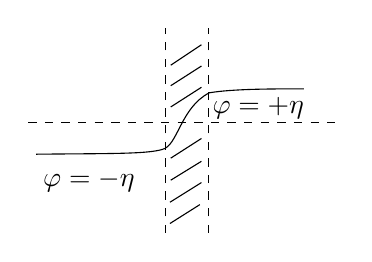
\begin{tikzpicture}[x=1cm,y=1cm]
\draw[dashed] (-2,0)--(2,0);
\draw[dashed] (-0.26,-1.4)--(-0.26,1.2);
\draw[dashed] (0.29,-1.4)--(0.29,1.2);
\draw (-0.20,-1.28)--(0.18,-1.04);
\draw (-0.20,-1.01)--(0.20,-0.76);
\draw (-0.19,-0.73)--(0.20,-0.49);
\draw (-0.19,-0.45)--(0.20,-0.20);
\draw (-0.19,0.20)--(0.20,0.45);
\draw (-0.19,0.47)--(0.20,0.72);
\draw (-0.19,0.73)--(0.20,0.99);
\draw (-1.90,-0.40)..controls(-1,-0.39)and(-0.5,-0.40)..(-0.3,-0.34)
 ..controls(-0.10,-0.30)and(-0.07,0.19)..(0.30,0.38)
 ..controls(0.60,0.43)and(1.10,0.43)..(1.50,0.43);
\node[below] at(-1.23,-0.48){$\varphi=-\eta$};
\node[below] at(0.92,0.45){$\varphi=+\eta$};
\end{tikzpicture}
\end{adjustbox}
\end{center}
[Справа от рисунка:] Рассм. стенку — \underline{реш., локализ. на плоскости.}
\begin{equation*}
\varphi=\varphi(x,y,z)\qquad(\text{не зав. от }t)
\end{equation*}
\begin{equation*}
\Box\varphi+\varphi\lambda^2(\varphi^2-\eta^2)=0
\qquad\text{— ур-е Эйлера для лагр. (2)}
\tag{6}
\end{equation*}
[\Unclear{GELFAND-P001070}{eq06-coefficient}{перед $\lambda^2$: $\varphi$ / $4$; множитель $4\varphi$ не восстановлен}]

(7) [Слева двойная вертикальная черта.]
$\underset{z\to\pm\infty}{\varphi=\pm\eta}$
от $x,y,z$ не зависит $\Rightarrow$ легко пров., что такое реш. сущ.

\SourcePage{GELFAND-P001071}{unlabelled}
% Full original scan frame inspected; manuscript regions read top-to-bottom.
% Review crops: original-pixel bbox [x0,y0,x1,y1), origin top left; nearest-neighbour scale.
% REVIEW top bbox=[95, 43, 2273, 1019] scale=3.0x
% REVIEW middle bbox=[81, 969, 2320, 1924] scale=3.0x
% REVIEW lower bbox=[83, 1907, 2313, 2907] scale=3.0x
% REVIEW bottom bbox=[83, 2905, 2408, 3415] scale=3.0x
% REVIEW continuous-group bbox=[974, 582, 1309, 689] scale=5.0x
% REVIEW before-solution-mark bbox=[397, 337, 477, 439] scale=9.0x
% REVIEW diagram14 bbox=[318, 2380, 644, 2950] scale=5.0x
% REVIEW overdrawn-arrow bbox=[1050, 2301, 1202, 2396] scale=8.0x
% REVIEW condition-ending bbox=[1472, 2470, 1810, 2572] scale=5.0x
% REVIEW solution-heading bbox=[276, 2978, 596, 3109] scale=5.0x
% REVIEW parenthesis-word bbox=[995, 3149, 1463, 3294] scale=6.0x
% REVIEW continuous-word bbox=[762, 572, 1014, 684] scale=6.0x
$\eta\sim m$

(8) Толщина слоя [вставлено снизу: (в (5))] $\sim\dfrac1\eta$.

[\Unclear{GELFAND-P001071}{before-solution05}{зачёркнутый знак неразборчив}] Реш. (5) явно нах.: \underline{\underline{$\operatorname{th}(z\eta)$}}

\underline{Гр. симметрии}: $\varphi\mapsto-\varphi$.

Сейчас обычно рассм. непр. гр. $G$ симм. лагранжиана.

$U(1)$-инвар. теория:
\begin{equation*}
\mathcal{L}(\varphi)=\frac12\bigl|(\partial_i+iA_i)\varphi\bigr|^2-(\varphi\varphi^*-\eta^2)^2
\tag{9}
\end{equation*}
\begin{equation*}
\text{Вакуум: }(c_1,c_2):\quad c_1^2+c_2^2=\eta^2
\tag{10}
\end{equation*}
(11)
\begin{center}
\begin{adjustbox}{max width=\linewidth}
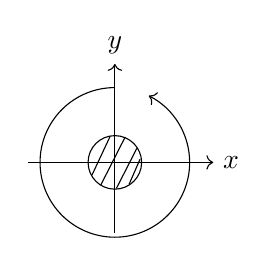
\begin{tikzpicture}[x=1cm,y=1cm]
\draw[->] (-1.10,0)--(1.25,0)node[right]{$x$};
\draw[->] (0,-0.90)--(0,1.25)node[above]{$y$};
\draw (0,0)circle(0.34);
\draw (-0.29,-0.16)--(-0.06,0.33);
\draw (-0.18,-0.29)--(0.13,0.32);
\draw (0.02,-0.33)--(0.28,0.18);
\draw (0.18,-0.28)--(0.32,0.04);
\draw[->] (0,0.95)arc[start angle=90,end angle=423,radius=0.95];
\end{tikzpicture}
\end{adjustbox}
\end{center}
[Справа от рисунка:] струна: когда энергия соср. на линии (1-мерной).

При обходе вектор $C$ поворач. на $2\pi$

Топологич. инвариант есть.

(Статическое решение: не зав. от $t$)

$A$ — доп. вект. поле (эл.-магн.)
\begin{equation*}
\mathcal{L}=-\frac14F_{ik}F_{ik}+\frac12\bigl|(\partial_i+iA_i)\varphi\bigr|^2-(\varphi\varphi^*-\eta^2)^2
\tag{12}
\end{equation*}
\begin{equation*}
F_{ik}=\partial_i A_k-\partial_k A_i
\end{equation*}
Действие $U(1)$ на поле:
\begin{equation*}
\begin{cases}
\varphi\mapsto e^{i\alpha}\varphi\\
A_i\mapsto A_i+\nabla_i\alpha
\end{cases}
\tag{13}
\end{equation*}
[\Unclear{GELFAND-P001071}{eq13-gauge-sign}{знаки $+iA_i$ и $A_i+\nabla_i\alpha$ сохранены}]

Рассм. приближ. решение [\Unclear{GELFAND-P001071}{after-approximate-solution}{зачёркнутый номер в скобках / перечёркнутая стрелка влево}]

(14) \SourceFigure{GELFAND-P001071}{diagram14}{Рис. (14): изогнутая узкая полоса, поперечные штрихи, выделенный участок у перегиба; к перегибу стрелка с подписью $r_{\mathrm{кр}}$, выше короткая стрелка влево. Штрихи внутри участка могут быть стрелками; см. оригинал.}

[Справа от рисунка, стрелка влево:] \underline{примем это за начальные условие}

Примерн. вид решения (11):
\begin{equation*}
\begin{cases}
\varphi_1=\dfrac xr f(r)\\
\varphi_2=\dfrac yr f(r)
\end{cases}
\tag{15}
\end{equation*}
(для \Unclear{GELFAND-P001071}{eq15-parenthesis-word}{неразборчиво; «…верста» / «…вёрста»?})

[Справа:] так же конструир. $A$

$\varepsilon(r)$ — плотность энергии в (11) — вычисляется.

\SourcePage{GELFAND-P001072}{67}
% Full original scan frame inspected; manuscript regions read top-to-bottom.
% Review crops: original-pixel bbox [x0,y0,x1,y1), origin top left; nearest-neighbour scale.
% REVIEW top bbox=[81, 48, 2370, 1059] scale=3.0x
% REVIEW middle bbox=[150, 1026, 2389, 1924] scale=3.0x
% REVIEW lower bbox=[57, 1860, 2377, 2860] scale=3.0x
% REVIEW bottom bbox=[52, 2791, 2377, 3382] scale=3.0x
% REVIEW top-cancellation bbox=[209, 59, 684, 183] scale=6.0x
% REVIEW coefficient17 bbox=[986, 646, 1100, 822] scale=8.0x
% REVIEW inside-string-insertion bbox=[929, 1066, 1135, 1214] scale=7.0x
% REVIEW use-invariance bbox=[530, 1530, 836, 1674] scale=6.0x
% REVIEW endpoints-text bbox=[762, 2432, 1758, 2556] scale=5.0x
% REVIEW diagram20 bbox=[256, 2938, 598, 3213] scale=6.0x
% REVIEW area-word bbox=[670, 3175, 1456, 3342] scale=5.0x
% REVIEW inside-string-abbreviation bbox=[762, 1057, 924, 1235] scale=7.0x
[Зачёркнуто: \Unclear{GELFAND-P001072}{top-cancelled-reference}{возможно «Решение»; далее (14)}.]

Должны вых. на вакуум: $\varphi_1^2+\varphi_2^2\to\eta^2$ при $r\to\infty$.

Локально (14) похоже на (11).

(16) Пусть радиус кривизны $r_{\mathrm{кр}}\gg\dfrac1\eta$

Эфф. действие: [стрелка вправо, затем вниз к правой части (17)]
\begin{equation*}
S=\int\mathcal{L}(\varphi)\,d^4x\simeq\nu\int dl\sqrt{1-v_{\perp}^2}\,dt
\tag{17}
\end{equation*}
[Справа сверху, стрелка влево-вниз к интегралу:] интеграл по самой струне.

$v_{\perp}$ — поперечная скор. струны

[Двойная вертикальная черта.] $\nu$ — линейная плотность энергии струны.

Эволюция — ?

Внутри струны счит. [вставлено сверху: что] ничего не происходит
(счит. [вставлено сверху: толщину] её дост. малой — — по сравнению с радиусами кривизны)

Интеграл вычисляем в каждом трансверс. сечении — получим $\nu$

$\sqrt{1-v_{\perp}^2}$ получается из $d^4x$ (заменой переменных)

Или: воспольз. релятивистской инвар.: $ds$ (интервал), запис. в $\forall$ сист. координат.

(17) — ф-ла \underline{Намбу}.

Можно рассм. кольцевую струну с лагранж. — пр. часть (17)

(18)
\begin{center}
\begin{adjustbox}{max width=\linewidth}
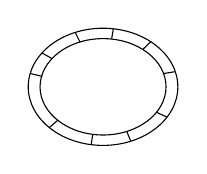
\begin{tikzpicture}[x=1cm,y=1.2cm]
\draw (0,0)ellipse(0.95 and 0.62);
\draw (0,0)ellipse(0.80 and 0.51);
\draw (-0.92,0.14)--(-0.77,0.11);
\draw (-0.78,0.36)--(-0.65,0.30);
\draw (-0.35,0.57)--(-0.29,0.47);
\draw (0.13,0.61)--(0.11,0.51);
\draw (0.61,0.48)--(0.51,0.40);
\draw (0.91,0.16)--(0.77,0.14);
\draw (0.81,-0.32)--(0.68,-0.27);
\draw (0.35,-0.57)--(0.30,-0.47);
\draw (-0.15,-0.61)--(-0.13,-0.50);
\draw (-0.68,-0.43)--(-0.57,-0.35);
\end{tikzpicture}
\end{adjustbox}
\end{center}
оно будет сжиматься, быстро вых. на световую скорость и сжимается в комочек.

\underline{Вариант.}

обрыв концов (сажаем на них по монополю):

(19)
\begin{center}
\begin{adjustbox}{max width=\linewidth}
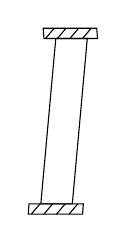
\begin{tikzpicture}[x=1cm,y=1cm]
\draw (-0.17,-1.1)--(0.02,1.0)--(0.42,1.0)--(0.23,-1.1)--cycle;
\draw (-0.13,1.00)--(0.55,1.00)--(0.54,1.13)--(-0.14,1.13)--cycle;
\draw (-0.11,1.00)--(0.00,1.13);
\draw (0.04,1.00)--(0.15,1.13);
\draw (0.20,1.00)--(0.31,1.13);
\draw (0.36,1.00)--(0.47,1.13);
\draw (-0.32,-1.10)--(0.37,-1.10)--(0.36,-1.23)--(-0.33,-1.23)--cycle;
\draw (-0.29,-1.23)--(-0.18,-1.10);
\draw (-0.13,-1.23)--(-0.02,-1.10);
\draw (0.03,-1.23)--(0.14,-1.10);
\draw (0.19,-1.23)--(0.30,-1.10);
\end{tikzpicture}
\end{adjustbox}
\end{center}
(20) \SourceFigure{GELFAND-P001072}{diagram20}{Рис. (20): искривлённая пластина с четырьмя внутренними поперечными дугами; справа $t=t_2$, $t=t_1$, снизу $t=0$. Неясно, все ли клиновидные окончания дуг являются стрелками.}

[Справа от рисунка:] при движении струна заметает пластину.

(21) \underline{Площадь заметаемой поверхности и есть лагранжиан ($17_{\mathrm{пр}}$)}

\SourcePage{GELFAND-P001073}{unlabelled}
% Full original scan frame inspected; manuscript regions read top-to-bottom.
% Review crops: original-pixel bbox [x0,y0,x1,y1), origin top left; nearest-neighbour scale.
% REVIEW top bbox=[43, 33, 2306, 872] scale=3.0x
% REVIEW middle bbox=[57, 872, 2392, 1579] scale=3.0x
% REVIEW lower bbox=[36, 1508, 2351, 2230] scale=3.0x
% REVIEW bottom bbox=[50, 2173, 2263, 2677] scale=3.0x
% REVIEW minimum-area-word bbox=[629, 190, 1154, 309] scale=6.0x
% REVIEW field-symbol22 bbox=[625, 551, 1159, 691] scale=6.0x
% REVIEW generator-cancellation bbox=[382, 1499, 494, 1598] scale=8.0x
% REVIEW overwritten-u25 bbox=[1401, 1966, 1594, 2161] scale=7.0x
% REVIEW overwritten-u25-detail bbox=[1572, 1971, 1682, 2123] scale=9.0x
$\dot x=\dfrac{\partial x}{\partial t}$, $x'=\dfrac{\partial x}{\partial s}$, $x(t,s)$ и считаем.

Возникает $\min$ площадь. [\Unclear{GELFAND-P001073}{minimum-area-ending}{окончание: «площадь» / «площади»}]

\underline{Струны и хромодинамика.}

\underline{Квант. хромодинамика:}
\begin{equation*}
\mathcal{L}(\Psi,A)=-\frac14F_{ik}^aF_{ik}^a+\bar\Psi(i\hat\partial-m)\Psi
\tag{22}
\end{equation*}
$a=1\div8$; $i,k=0,1,2,3$.
\begin{equation*}
\hat\partial=\gamma^i(\partial_i+iI^aA_i^a)
\tag{23}
\end{equation*}
[Под $\gamma^i$, соединено короткой вертикальной чертой:] матр. Дирака
\begin{equation*}
F_{ik}^a=\partial_i A_k^a-\partial_k A_i^a+g f_{abc}A_i^bA_k^c,
\tag{24}
\end{equation*}
$g$ — конст. связи, $f_{abc}$ — структ. постоянные группы.

\underline{Действует}: группа $SU(3)$ (присоед. предст.) — отсюда 8.

— действует на $A$

[Зачёркнуто: \Unclear{GELFAND-P001073}{before-generator-ia}{возможно $a$; зачёркнутый знак неразборчив}]

$I^a$ — генер. $SU(3)$, $I^a=I^a_{\alpha\beta}$.

в $\bar\Psi$ и $\Psi$ есть ещё цветовой индекс (кварки-триплеты) — — по нему делается свёртка.

На самом деле надо неск. типов кварков. хотя бы 2 типа
\begin{equation*}
\mathcal{L}(\Psi,A)=-\frac14F_{ik}^aF_{ik}^a+\bar u(i\hat\partial-m)u+\bar d(i\hat\partial-m)d
\tag{25}
\end{equation*}
[\Unclear{GELFAND-P001073}{eq25-overwritten-field}{$u$ после первой скобки густо переписано; предыдущее начертание не установлено}]

($u$-кварки и $d$-кварки)
\begin{equation*}
\hat\partial_i=\nabla_i+iA_i^a I^a,\qquad I^a=I^a_{\alpha\beta}
\tag{26}
\end{equation*}
$A$ — поле Я.-М. или \underline{глюонное} (склеивает кварки)

(gluon field)


\end{document}
